\chapter{虚拟装备中的形式∞-范畴论}\label{ch:formal-infinity-category-theory}


Mac Lane 有一句著名的断言：「一切概念皆是\trKanExtension」[81, \S X.7]，至少
在范畴论中是如此。\trFunctor{} $f\colon A\to C$ 沿\trFunctor{} $k\colon A\to B$
的右\trExtension{}与左\trExtension{}可以在任何 2-范畴的内部定义（见%
\cref{def:two-categorical-extension}）——在这一般性层面上，「Kan」这一名号
通常会被省去。然而，在一个\trInfinityCosmos{}的\trHomotopyTwoCategory{}中，
定义左\trExtension{}与右\trExtension{}的\trUniversalProperty{}过弱；事实上，
正确的\trUniversalProperty{}隶属于一个更强的概念——\emph{\trPointwiseExtension}
（pointwise extension）：对于\trPointwiseExtension，右\trExtension{}或左%
\trExtension{}在 $B$ 的一个\trElement{}处取的值，可以作为以相应的%
\trCommaInfinityCategory{}为指标的\trLimit{}或\trColimit{}来计算（命题 9.4.9
给出精确表述）。的确，Kelly 后来修正了 Mac Lane 的断言，主张\emph{逐点%
\trKanExtension}——他径直称之为「\trKanExtension」——才是重要的那些，并写道：
「我们现今对命名法的抉择，基于我们未能找到一个单独的实例，使某个［非逐点的］%
\trKanExtension{}在其中扮演丝毫数学角色」[68, \S 4]。

利用模的演算，我们现在可以把\trInfinityCategories{}之间的\trFunctor{}的逐点%
\trKanExtension{}理论，添入第一部分中发展的基础∞-范畴论之中。事实上，我们对%
\trPointwiseExtension{}给出多种定义。其中一种在本质上是 2-范畴式的：\trPointwiseExtension{}是%
\trHomotopyTwoCategory{}中一个寻常的 2-范畴式\trExtension，它对与\trCommaSquare
（comma square）的粘贴稳定。另一定义则是：一个\trNaturalTransformation{}定义
一个逐点右\trExtension{}，当且仅当它在向模的\trVirtualEquipment{}的共变嵌入
（covariant embedding）之下的像，在该\trVirtualEquipment{}中定义一个右%
\trExtension。定理 9.3.3 证明这两个概念重合。

在 9.1 节中，我们在模的\trVirtualEquipment{}中引入右\trLifting{}与右%
\trExtension，并建立它们的初等性质。在把注意力转向\trPointwiseExtension{}之前，
我们先在 9.2 节中引入\emph{\trExactSquare}（exact squares）——%
\trHomotopyTwoCategory{}中的一族方块，其中包含\trCommaSquare——它们被用来在%
\trHomotopyTwoCategory{}的内部刻画\trPointwiseExtension。\trPointwiseExtension{}将在
9.3 节中以多种等价的方式引入，并在 9.4 节中投入运用，以发展形式∞-范畴论的
若干侧面。

9.4 节的探讨以对\trAdjunction{}与\trFullyFaithful{}\trFunctor{}的讨论开篇，
重访早已踏熟的领域。逐点右\trExtension{}与左\trExtension{}至关紧要的应用
出现在该节的后半部分：在那里，我们在不必是\trCartesianClosed{}一般%
\trInfinityCosmos{}中，定义以\trInfinityCategory{}为指标的图表的\trLimit{}与%
\trColimit。在 9.5 节中，我们对\trInfinityCategories{}之间的图表引入更一般的
一类\trLimit{}与\trColimit{}——即由一个任意\trModule{}\emph{加权}（weighted）
的图表——并迅速建立\trWeightedLimit{}与\trWeightedColimit{}之演算的关键组成部分。
这些结果可以被理解为揭示出：\trInfinityCategories{}的许多方面都自动地富集于%
\trDiscrete{}\trInfinityCategories{}之上。

有一个问题我们在本章不予讨论：即保证逐点左\trExtension{}与右\trExtension{}之
存在性的判据。我们将在 12.3 节中重返这一话题——在那里，我们利用第 12 章中
建立的关于逐点定义的\trUniversalProperty{}的诸结果，在一个由 $(\infty,1)$-范畴
组成的\trInfinityCosmos{}中证明命题 9.4.9 所预期的逆命题，从而把逐点左%
\trExtension{}或右\trExtension{}的存在性问题约化为某些\trColimit{}或\trLimit{}%
的存在性问题。


\section{模的\trLifting{}与\trExtension}\label{sec:liftings-and-extensions-of-modules}

在本节中，我们在模的\trVirtualEquipment{}中引入并研究\trLifting{}与%
\trExtension{}。为给\cref{def:right-extension-lifting-modules}提供动机，我们
先简要回忆那个标准的 2-范畴式概念：

\begin{definition}\label{def:two-categorical-extension}
1-\trCell{} $f\colon A\to C$ 沿 1-\trCell{} $k\colon A\to B$ 的一个%
\textbf{右扩张}（right extension），由一个数对
$(r\colon B\to C,\ \nu\colon rk\Rightarrow f)$ 给出，如下左图所示
\begin{center}
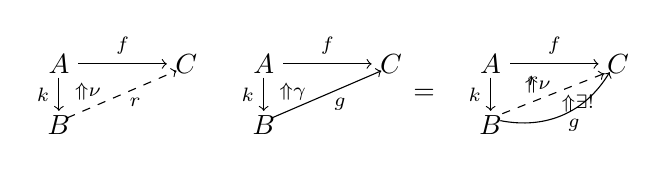
\begin{tikzpicture}[x=1em,y=1em]
  \node at (0,2.2)   {$A$};
  \node at (4.6,2.2) {$C$};
  \node at (0,0)     {$B$};
  \draw[->] (0.7,2.2) -- node[above]{$\scriptstyle f$} (3.9,2.2);
  \draw[->] (0,1.7)   -- node[left]{$\scriptstyle k$} (0,0.5);
  \draw[->,dashed] (0.3,0.25) -- node[below,pos=0.62]{$\scriptstyle r$} (4.25,1.95);
  \node at (1.05,1.2) {$\scriptstyle\Uparrow\nu$};
  \begin{scope}[shift={(7.4,0)}]
    \node at (0,2.2)   {$A$};
    \node at (4.6,2.2) {$C$};
    \node at (0,0)     {$B$};
    \draw[->] (0.7,2.2) -- node[above]{$\scriptstyle f$} (3.9,2.2);
    \draw[->] (0,1.7)   -- node[left]{$\scriptstyle k$} (0,0.5);
    \draw[->] (0.3,0.25) -- node[below,pos=0.62]{$\scriptstyle g$} (4.25,1.95);
    \node at (1.05,1.2) {$\scriptstyle\Uparrow\gamma$};
  \end{scope}
  \node at (13.2,1.1) {$=$};
  \begin{scope}[shift={(15.6,0)}]
    \node at (0,2.2)   {$A$};
    \node at (4.6,2.2) {$C$};
    \node at (0,0)     {$B$};
    \draw[->] (0.7,2.2) -- node[above]{$\scriptstyle f$} (3.9,2.2);
    \draw[->] (0,1.7)   -- node[left]{$\scriptstyle k$} (0,0.5);
    \draw[->,dashed] (0.42,0.4) -- node[above left,pos=0.45]{$\scriptstyle r$} (4.1,1.85);
    \draw[->] (0.35,0.15) to[bend right=35] node[below,pos=0.6]{$\scriptstyle g$} (4.3,1.9);
    \node at (1.7,1.45)  {$\scriptstyle\Uparrow\nu$};
    \node at (3.15,0.75) {$\scriptstyle\Uparrow\exists!$};
  \end{scope}
\end{tikzpicture}
\end{center}
使得任何如中图所示的那类数对都经由 $\nu$ 唯一地分解，如上右图所示。

对偶地，1-\trCell{} $f\colon A\to C$ 沿 1-\trCell{} $k\colon A\to B$ 的一个%
\textbf{左扩张}（left extension），由一个数对
$(\ell\colon B\to C,\ \lambda\colon f\Rightarrow \ell k)$ 给出，如下左图所示
\begin{center}
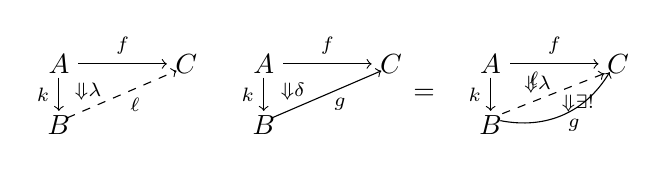
\begin{tikzpicture}[x=1em,y=1em]
  \node at (0,2.2)   {$A$};
  \node at (4.6,2.2) {$C$};
  \node at (0,0)     {$B$};
  \draw[->] (0.7,2.2) -- node[above]{$\scriptstyle f$} (3.9,2.2);
  \draw[->] (0,1.7)   -- node[left]{$\scriptstyle k$} (0,0.5);
  \draw[->,dashed] (0.3,0.25) -- node[below,pos=0.62]{$\scriptstyle\ell$} (4.25,1.95);
  \node at (1.05,1.2) {$\scriptstyle\Downarrow\lambda$};
  \begin{scope}[shift={(7.4,0)}]
    \node at (0,2.2)   {$A$};
    \node at (4.6,2.2) {$C$};
    \node at (0,0)     {$B$};
    \draw[->] (0.7,2.2) -- node[above]{$\scriptstyle f$} (3.9,2.2);
    \draw[->] (0,1.7)   -- node[left]{$\scriptstyle k$} (0,0.5);
    \draw[->] (0.3,0.25) -- node[below,pos=0.62]{$\scriptstyle g$} (4.25,1.95);
    \node at (1.05,1.2) {$\scriptstyle\Downarrow\delta$};
  \end{scope}
  \node at (13.2,1.1) {$=$};
  \begin{scope}[shift={(15.6,0)}]
    \node at (0,2.2)   {$A$};
    \node at (4.6,2.2) {$C$};
    \node at (0,0)     {$B$};
    \draw[->] (0.7,2.2) -- node[above]{$\scriptstyle f$} (3.9,2.2);
    \draw[->] (0,1.7)   -- node[left]{$\scriptstyle k$} (0,0.5);
    \draw[->,dashed] (0.42,0.4) -- node[above left,pos=0.45]{$\scriptstyle\ell$} (4.1,1.85);
    \draw[->] (0.35,0.15) to[bend right=35] node[below,pos=0.6]{$\scriptstyle g$} (4.3,1.9);
    \node at (1.7,1.45)  {$\scriptstyle\Downarrow\lambda$};
    \node at (3.15,0.75) {$\scriptstyle\Downarrow\exists!$};
  \end{scope}
\end{tikzpicture}
\end{center}
使得任何如中图所示的那类数对都经由 $\lambda$ 唯一地分解，如上右图所示。
\end{definition}

\cref{def:two-categorical-extension}的诸 op-对偶在任何 2-范畴中定义了%
\textbf{右\trLifting}（right lifting）与\textbf{左\trLifting}（left lifting）图。
对于\trVirtualDoubleCategory{}中的水平箭头，也能定义类似的右扩张与右提升
概念；而凡当\trVirtualEquipment{}拥有其限制（restriction）时，只需考虑那些
竖直边缘箭头皆为恒同的「纤维化」胞腔便已足够。
我们于是把用语专门化到模的\trVirtualEquipment{}，因为这正是我们感兴趣的
场合：

\begin{definition}\label{def:right-extension-lifting-modules}
模 $A\xrightarrow{F}C$ 沿模 $A\xrightarrow{K}B$ 的一个\textbf{右扩张}，由
一支模 $B\xrightarrow{R}C$ 连同一个二元\trCell{}一起构成的数对给出
\begin{center}
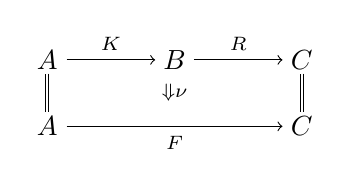
\begin{tikzpicture}[x=1em,y=1em]
  \node at (0,1.2)    {$A$};
  \node at (4.6,1.2)  {$B$};
  \node at (9.2,1.2)  {$C$};
  \node at (0,-1.2)   {$A$};
  \node at (9.2,-1.2) {$C$};
  \draw[->] (0.7,1.2)  -- node[above]{$\scriptstyle K$} (3.9,1.2);
  \draw[->] (5.3,1.2)  -- node[above]{$\scriptstyle R$} (8.5,1.2);
  \draw[->] (0.7,-1.2) -- node[below]{$\scriptstyle F$} (8.5,-1.2);
  \draw[double] (0,0.7)   -- (0,-0.7);
  \draw[double] (9.2,0.7) -- (9.2,-0.7);
  \node at (4.6,0) {$\scriptstyle\Downarrow\nu$};
\end{tikzpicture}
\end{center}
它具有如下性质：每一个形如下左图所示的 $n+1$ 元\trCell{}都经由
$\nu\colon K\divideontimes R\Rightarrow F$ 唯一地分解，如下右图所示：
\begin{center}
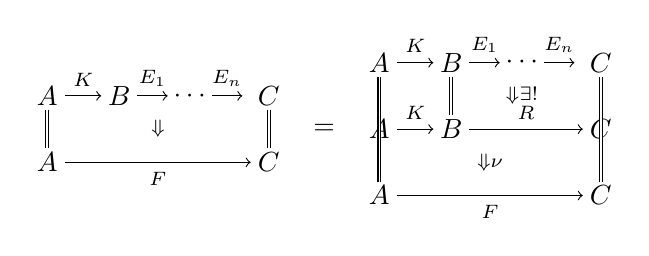
\begin{tikzpicture}[x=1em,y=1em]
  \begin{scope}
    \node at (0,1.2)   {$A$};
    \node at (2.6,1.2) {$B$};
    \node at (8.0,1.2) {$C$};
    \draw[->] (0.65,1.2) -- node[above]{$\scriptstyle K$} (1.95,1.2);
    \draw[->] (3.25,1.2) -- node[above]{$\scriptstyle E_{1}$} (4.35,1.2);
    \node at (5.15,1.2)  {$\cdots$};
    \draw[->] (5.95,1.2) -- node[above]{$\scriptstyle E_{n}$} (7.05,1.2);
    \node at (0,-1.2)    {$A$};
    \node at (8.0,-1.2)  {$C$};
    \draw[->] (0.65,-1.2) -- node[below]{$\scriptstyle F$} (7.35,-1.2);
    \draw[double] (0,0.7)   -- (0,-0.7);
    \draw[double] (8.0,0.7) -- (8.0,-0.7);
    \node at (4.0,0) {$\scriptstyle\Downarrow$};
  \end{scope}
  \node at (10.0,0) {$=$};
  \begin{scope}[shift={(12.0,0)}]
    \node at (0,2.4)   {$A$};
    \node at (2.6,2.4) {$B$};
    \node at (8.0,2.4) {$C$};
    \draw[->] (0.65,2.4) -- node[above]{$\scriptstyle K$} (1.95,2.4);
    \draw[->] (3.25,2.4) -- node[above]{$\scriptstyle E_{1}$} (4.35,2.4);
    \node at (5.15,2.4)  {$\cdots$};
    \draw[->] (5.95,2.4) -- node[above]{$\scriptstyle E_{n}$} (7.05,2.4);
    \node at (0,0)   {$A$};
    \node at (2.6,0) {$B$};
    \node at (8.0,0) {$C$};
    \draw[->] (0.65,0) -- node[above]{$\scriptstyle K$} (1.95,0);
    \draw[->] (3.25,0) -- node[above]{$\scriptstyle R$} (7.35,0);
    \node at (0,-2.4)   {$A$};
    \node at (8.0,-2.4) {$C$};
    \draw[->] (0.65,-2.4) -- node[below]{$\scriptstyle F$} (7.35,-2.4);
    \draw[double] (0,1.9)   -- (0,-1.9);
    \draw[double] (8.0,1.9) -- (8.0,-1.9);
    \draw[double] (2.6,1.9) -- (2.6,0.5);
    \node at (5.15,1.2) {$\scriptstyle\Downarrow\exists!$};
    \node at (4.0,-1.2) {$\scriptstyle\Downarrow\nu$};
  \end{scope}
\end{tikzpicture}
\end{center}

对偶地，模 $A\xrightarrow{F}C$ 穿过模 $B\xrightarrow{H}C$ 的一个%
\textbf{右提升}，由一支模 $A\xrightarrow{L}B$ 连同一个二元\trCell{}一起构成
的数对给出
\begin{center}
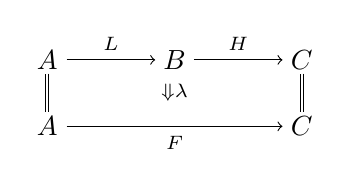
\begin{tikzpicture}[x=1em,y=1em]
  \node at (0,1.2)    {$A$};
  \node at (4.6,1.2)  {$B$};
  \node at (9.2,1.2)  {$C$};
  \node at (0,-1.2)   {$A$};
  \node at (9.2,-1.2) {$C$};
  \draw[->] (0.7,1.2)  -- node[above]{$\scriptstyle L$} (3.9,1.2);
  \draw[->] (5.3,1.2)  -- node[above]{$\scriptstyle H$} (8.5,1.2);
  \draw[->] (0.7,-1.2) -- node[below]{$\scriptstyle F$} (8.5,-1.2);
  \draw[double] (0,0.7)   -- (0,-0.7);
  \draw[double] (9.2,0.7) -- (9.2,-0.7);
  \node at (4.6,0) {$\scriptstyle\Downarrow\lambda$};
\end{tikzpicture}
\end{center}
它具有如下性质：每一个形如下左图所示的 $n+1$ 元\trCell{}都经由
$\lambda\colon L\divideontimes H\Rightarrow F$ 唯一地分解，如下右图所示：
\begin{center}
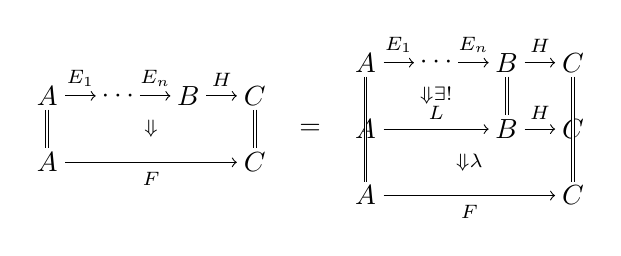
\begin{tikzpicture}[x=1em,y=1em]
  \begin{scope}
    \node at (0,1.2)   {$A$};
    \node at (5.1,1.2) {$B$};
    \node at (7.5,1.2) {$C$};
    \draw[->] (0.65,1.2) -- node[above]{$\scriptstyle E_{1}$} (1.75,1.2);
    \node at (2.55,1.2)  {$\cdots$};
    \draw[->] (3.35,1.2) -- node[above]{$\scriptstyle E_{n}$} (4.45,1.2);
    \draw[->] (5.75,1.2) -- node[above]{$\scriptstyle H$} (6.85,1.2);
    \node at (0,-1.2)    {$A$};
    \node at (7.5,-1.2)  {$C$};
    \draw[->] (0.65,-1.2) -- node[below]{$\scriptstyle F$} (6.85,-1.2);
    \draw[double] (0,0.7)   -- (0,-0.7);
    \draw[double] (7.5,0.7) -- (7.5,-0.7);
    \node at (3.75,0) {$\scriptstyle\Downarrow$};
  \end{scope}
  \node at (9.5,0) {$=$};
  \begin{scope}[shift={(11.5,0)}]
    \node at (0,2.4)   {$A$};
    \node at (5.1,2.4) {$B$};
    \node at (7.5,2.4) {$C$};
    \draw[->] (0.65,2.4) -- node[above]{$\scriptstyle E_{1}$} (1.75,2.4);
    \node at (2.55,2.4)  {$\cdots$};
    \draw[->] (3.35,2.4) -- node[above]{$\scriptstyle E_{n}$} (4.45,2.4);
    \draw[->] (5.75,2.4) -- node[above]{$\scriptstyle H$} (6.85,2.4);
    \node at (0,0)   {$A$};
    \node at (5.1,0) {$B$};
    \node at (7.5,0) {$C$};
    \draw[->] (0.65,0) -- node[above]{$\scriptstyle L$} (4.45,0);
    \draw[->] (5.75,0) -- node[above]{$\scriptstyle H$} (6.85,0);
    \node at (0,-2.4)   {$A$};
    \node at (7.5,-2.4) {$C$};
    \draw[->] (0.65,-2.4) -- node[below]{$\scriptstyle F$} (6.85,-2.4);
    \draw[double] (0,1.9)   -- (0,-1.9);
    \draw[double] (7.5,1.9) -- (7.5,-1.9);
    \draw[double] (5.1,1.9) -- (5.1,0.5);
    \node at (2.55,1.2) {$\scriptstyle\Downarrow\exists!$};
    \node at (3.75,-1.2) {$\scriptstyle\Downarrow\lambda$};
  \end{scope}
\end{tikzpicture}
\end{center}
\end{definition}

由于第 8 章中的\cref{def:virtual-double-category}存在着不对称性，并没有相应
的左扩张或左提升概念。
由这些定义容易得出：诸右扩张或诸右提升均在 $\mathbb{M}od(\mathcal{K})$ 中在
竖直同构的意义下唯一（见\cref{ex:uniqueness-right-extensions}）。

\begin{lemma}\label{lem:hom-binary-cell}
对任意\trFunctor{} $f\colon A\to B$，存在一个二元\trCell{}
\begin{center}
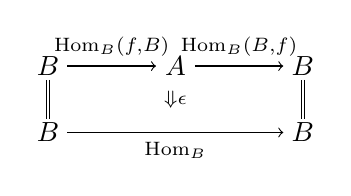
\begin{tikzpicture}[x=1em,y=1em]
  \node at (0,1.2)    {$B$};
  \node at (4.6,1.2)  {$A$};
  \node at (9.2,1.2)  {$B$};
  \node at (0,-1.2)   {$B$};
  \node at (9.2,-1.2) {$B$};
  \draw[->] (0.7,1.2)  -- node[above]{$\scriptstyle \mathrm{Hom}_{B}(f,B)$} (3.9,1.2);
  \draw[->] (5.3,1.2)  -- node[above]{$\scriptstyle \mathrm{Hom}_{B}(B,f)$} (8.5,1.2);
  \draw[->] (0.7,-1.2) -- node[below]{$\scriptstyle \mathrm{Hom}_{B}$} (8.5,-1.2);
  \draw[double] (0,0.7)   -- (0,-0.7);
  \draw[double] (9.2,0.7) -- (9.2,-0.7);
  \node at (4.6,0) {$\scriptstyle\Downarrow\epsilon$};
\end{tikzpicture}
\end{center}
它同时定义了 $B\xrightarrow{\mathrm{Hom}_{B}}B$ 穿过
$B\xrightarrow{\mathrm{Hom}_{B}(f,B)}A$ 的一个右扩张，以及
$B\xrightarrow{\mathrm{Hom}_{B}}B$ 穿过
$A\xrightarrow{\mathrm{Hom}_{B}(B,f)}B$ 的一个右提升。
\end{lemma}

\begin{proof}
二元胞腔 $\epsilon\colon \mathrm{Hom}_{B}(f,B)\divideontimes \mathrm{Hom}_{B}(B,f)\Rightarrow \mathrm{Hom}_{B}$（它也作为某种余单位出现在练习 8.4.v 中）在定理
8.4.4 与命题 8.2.4 的双射之下对应于一元单位胞腔 $\mathrm{Hom}_{f}$。
诸泛性质的验证留作\cref{ex:hom-cell-universal-properties}。
\end{proof}

\cref{lem:hom-binary-cell}的结果是一族更一般的例子之特例：

\begin{lemma}\label{lem:canonical-restriction-cells}
对任意模 $A\xrightarrow{E}B$ 与任意一对\trFunctor{} $g\colon C\to A$、
$f\colon D\to B$，诸典范\trCell
\begin{center}
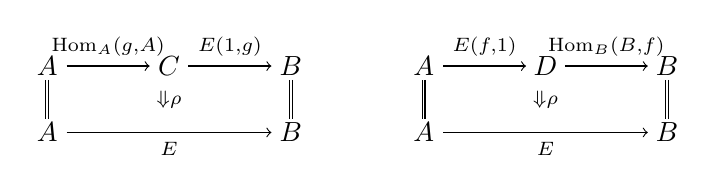
\begin{tikzpicture}[x=1em,y=1em]
  \begin{scope}
    \node at (0,1.2)   {$A$};
    \node at (4.4,1.2) {$C$};
    \node at (8.8,1.2) {$B$};
    \node at (0,-1.2)  {$A$};
    \node at (8.8,-1.2){$B$};
    \draw[->] (0.7,1.2)  -- node[above]{$\scriptstyle \mathrm{Hom}_{A}(g,A)$} (3.7,1.2);
    \draw[->] (5.1,1.2)  -- node[above]{$\scriptstyle E(1,g)$} (8.1,1.2);
    \draw[->] (0.7,-1.2) -- node[below]{$\scriptstyle E$} (8.1,-1.2);
    \draw[double] (0,0.7)   -- (0,-0.7);
    \draw[double] (8.8,0.7) -- (8.8,-0.7);
    \node at (4.4,0) {$\scriptstyle\Downarrow\rho$};
  \end{scope}
  \begin{scope}[shift={(13.6,0)}]
    \node at (0,1.2)   {$A$};
    \node at (4.4,1.2) {$D$};
    \node at (8.8,1.2) {$B$};
    \node at (0,-1.2)  {$A$};
    \node at (8.8,-1.2){$B$};
    \draw[->] (0.7,1.2)  -- node[above]{$\scriptstyle E(f,1)$} (3.7,1.2);
    \draw[->] (5.1,1.2)  -- node[above]{$\scriptstyle \mathrm{Hom}_{B}(B,f)$} (8.1,1.2);
    \draw[->] (0.7,-1.2) -- node[below]{$\scriptstyle E$} (8.1,-1.2);
    \draw[double] (0,0.7)   -- (0,-0.7);
    \draw[double] (8.8,0.7) -- (8.8,-0.7);
    \node at (4.4,0) {$\scriptstyle\Downarrow\rho$};
  \end{scope}
\end{tikzpicture}
\end{center}
展现 $E(1,g)$ 为 $E$ 穿过 $\mathrm{Hom}_{A}(g,A)$ 的右扩张，并展现 $E(f,1)$
为 $E$ 穿过 $\mathrm{Hom}_{B}(B,f)$ 的右提升。
\end{lemma}

\begin{proof}
所述的诸典范\trCell{}定义为：把定理 8.4.4 的双射作用于命题 8.2.1 的诸限制%
\trCell{}；也就是说，就上方左图所示的右扩张图表而言，这个\trCell{}作为如下
复合而得到
\begin{center}
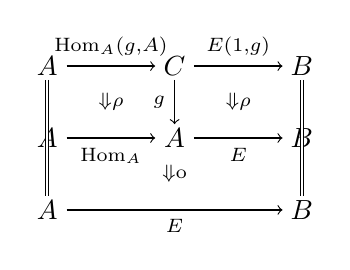
\begin{tikzpicture}[x=1em,y=1em]
  \node at (0,2.6)    {$A$};
  \node at (4.6,2.6)  {$C$};
  \node at (9.2,2.6)  {$B$};
  \node at (0,0)      {$A$};
  \node at (4.6,0)    {$A$};
  \node at (9.2,0)    {$B$};
  \node at (0,-2.6)   {$A$};
  \node at (9.2,-2.6) {$B$};
  \draw[->] (0.7,2.6)  -- node[above]{$\scriptstyle \mathrm{Hom}_{A}(g,A)$} (3.9,2.6);
  \draw[->] (5.3,2.6)  -- node[above]{$\scriptstyle E(1,g)$} (8.5,2.6);
  \draw[->] (0.7,0)    -- node[below]{$\scriptstyle \mathrm{Hom}_{A}$} (3.9,0);
  \draw[->] (5.3,0)    -- node[below]{$\scriptstyle E$} (8.5,0);
  \draw[->] (0.7,-2.6) -- node[below]{$\scriptstyle E$} (8.5,-2.6);
  \draw[double] (0,2.1)   -- (0,-2.1);
  \draw[double] (9.2,2.1) -- (9.2,-2.1);
  \draw[->] (4.6,2.1) -- node[left]{$\scriptstyle g$} (4.6,0.5);
  \node at (2.3,1.3)  {$\scriptstyle\Downarrow\rho$};
  \node at (6.9,1.3)  {$\scriptstyle\Downarrow\rho$};
  \node at (4.6,-1.3) {$\scriptstyle\Downarrow\mathrm{o}$};
\end{tikzpicture}
\end{center}
右扩张的泛性质由推论 8.4.6 提供。
\end{proof}

特别地：

\begin{corollary}\label{cor:module-self-extension}
任何模 $A\xrightarrow{E}B$ 都是它自身沿 $A\xrightarrow{\mathrm{Hom}_{A}}A$ 的
右扩张，同时也是它自身穿过 $B\xrightarrow{\mathrm{Hom}_{B}}B$ 的右提升。
\end{corollary}

诸右扩张与诸右提升分别可以理解为「在左侧与一支模作水平复合」和「在右侧与
一支模作水平复合」这两种运算的右伴随（见定理 12.3.6）。
由此引出下面这个「结合性」结果；我们就右扩张来陈述它，把右提升的对偶结果
留给读者。

\begin{proposition}\label{prop:right-extension-associativity}
设 $A\xrightarrow{K}B$、$B\xrightarrow{H}C$ 与 $A\xrightarrow{F}D$ 都是模，
使得复合 $K\otimes H$ 与右扩张 $B\xrightarrow{R_{K}F}D$ 存在。此时，
$R_{K}F$ 沿 $H$ 的右扩张存在，当且仅当 $F$ 沿 $K\otimes H$ 的右扩张存在；
而在二者存在时，$R_{H}(R_{K}F)\simeq_{C\times D}R_{K\otimes H}F$。
\end{proposition}

\begin{proof}
二元复合\trCell{} $\mu\colon K\divideontimes H\Rightarrow K\otimes H$ 的泛性质与右
扩张\trCell{} $\nu\colon K\divideontimes R_{K}F\Rightarrow F$ 一起，在涉及从 $C$ 到
$D$ 的模的任意相容序列 $R_{1}\divideontimes\cdots\divideontimes R_{n}$ 的诸\trCell{}之间
提供了如下双射（见记号 8.2.7）：
\begin{center}
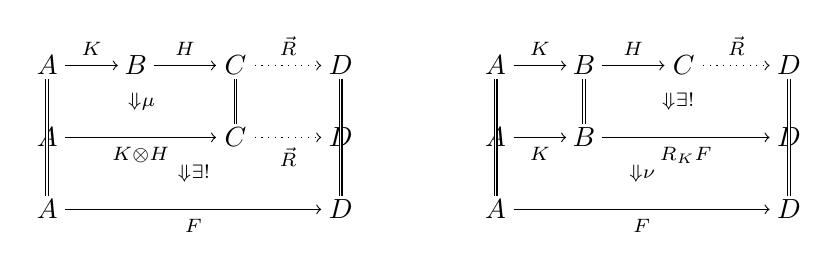
\begin{tikzpicture}[x=1em,y=1em]
  \begin{scope}
    \node at (0,2.6)    {$A$};
    \node at (3.2,2.6)  {$B$};
    \node at (6.8,2.6)  {$C$};
    \node at (10.6,2.6) {$D$};
    \draw[->] (0.65,2.6) -- node[above]{$\scriptstyle K$} (2.55,2.6);
    \draw[->] (3.85,2.6) -- node[above]{$\scriptstyle H$} (6.1,2.6);
    \draw[->,dotted] (7.5,2.6) -- node[above]{$\scriptstyle\vec{R}$} (9.9,2.6);
    \node at (0,0)    {$A$};
    \node at (6.8,0)  {$C$};
    \node at (10.6,0) {$D$};
    \draw[->] (0.65,0) -- node[below]{$\scriptstyle K\otimes H$} (6.1,0);
    \draw[->,dotted] (7.5,0) -- node[below]{$\scriptstyle\vec{R}$} (9.9,0);
    \node at (0,-2.6)   {$A$};
    \node at (10.6,-2.6){$D$};
    \draw[->] (0.65,-2.6) -- node[below]{$\scriptstyle F$} (9.9,-2.6);
    \draw[double] (0,2.1)    -- (0,-2.1);
    \draw[double] (10.6,2.1) -- (10.6,-2.1);
    \draw[double] (6.8,2.1)  -- (6.8,0.5);
    \node at (3.4,1.3)  {$\scriptstyle\Downarrow\mu$};
    \node at (5.3,-1.3) {$\scriptstyle\Downarrow\exists!$};
  \end{scope}
  \node at (13.4,0) {$\leftrightsquigarrow$};
  \begin{scope}[shift={(16.2,0)}]
    \node at (0,2.6)    {$A$};
    \node at (3.2,2.6)  {$B$};
    \node at (6.8,2.6)  {$C$};
    \node at (10.6,2.6) {$D$};
    \draw[->] (0.65,2.6) -- node[above]{$\scriptstyle K$} (2.55,2.6);
    \draw[->] (3.85,2.6) -- node[above]{$\scriptstyle H$} (6.1,2.6);
    \draw[->,dotted] (7.5,2.6) -- node[above]{$\scriptstyle\vec{R}$} (9.9,2.6);
    \node at (0,0)    {$A$};
    \node at (3.2,0)  {$B$};
    \node at (10.6,0) {$D$};
    \draw[->] (0.65,0) -- node[below]{$\scriptstyle K$} (2.55,0);
    \draw[->] (3.85,0) -- node[below]{$\scriptstyle R_{K}F$} (9.9,0);
    \node at (0,-2.6)   {$A$};
    \node at (10.6,-2.6){$D$};
    \draw[->] (0.65,-2.6) -- node[below]{$\scriptstyle F$} (9.9,-2.6);
    \draw[double] (0,2.1)    -- (0,-2.1);
    \draw[double] (10.6,2.1) -- (10.6,-2.1);
    \draw[double] (3.2,2.1)  -- (3.2,0.5);
    \node at (6.6,1.3)  {$\scriptstyle\Downarrow\exists!$};
    \node at (5.3,-1.3) {$\scriptstyle\Downarrow\nu$};
  \end{scope}
\end{tikzpicture}
\end{center}

在模的空序列的情形，这一双射在纤维化模映射 $K\otimes H\Rightarrow F$ 与纤维化
模映射 $H\Rightarrow R_{K}F$ 之间编码了一种伴随性。
若右扩张 $R_{K\otimes H}F$ 存在，我们就取它充当 $R$，并利用左下方的
二元\trCell{}去诱导右上方的二元\trCell{}；可以证明，这使得 $R_{K\otimes H}F$
表现为 $R_{K}F$ 沿 $H$ 的右扩张 $R_{H}(R_{K}F)$。
反之，若右扩张 $R_{H}(R_{K}F)$ 存在，我们就利用右上方的二元\trCell{}去诱导
左下方的二元\trCell{}；可以证明，这使得 $R_{H}(R_{K}F)$ 表现为 $F$ 沿
$K\otimes H$ 的右扩张 $R_{K\otimes H}F$。这种泛性质的转移是直截了当的，同样
由刚才展示的双射得出。

最后，若右扩张 $R_{H}(R_{K}F)$ 与 $R_{K\otimes H}F$ 分别已知存在，则上面的
论证结合右扩张的唯一性，便共同表明：作为从 $C$ 到 $D$ 的模，
$R_{K\otimes H}F\simeq R_{H}(R_{K}F)$（见\cref{ex:uniqueness-right-extensions}）。
\end{proof}

现在我们来说明\cref{def:right-extension-lifting-modules}如何经由定义 8.4.12
的共变嵌入与反变嵌入而与\cref{def:two-categorical-extension}相关联。

\begin{lemma}\label{lem:embedded-extension-lifting}
若
\begin{center}
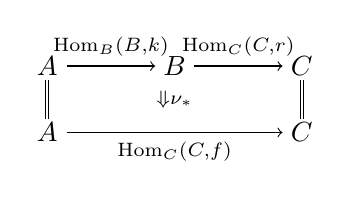
\begin{tikzpicture}[x=1em,y=1em]
  \node at (0,1.2)    {$A$};
  \node at (4.6,1.2)  {$B$};
  \node at (9.2,1.2)  {$C$};
  \node at (0,-1.2)   {$A$};
  \node at (9.2,-1.2) {$C$};
  \draw[->] (0.7,1.2)  -- node[above]{$\scriptstyle \mathrm{Hom}_{B}(B,k)$} (3.9,1.2);
  \draw[->] (5.3,1.2)  -- node[above]{$\scriptstyle \mathrm{Hom}_{C}(C,r)$} (8.5,1.2);
  \draw[->] (0.7,-1.2) -- node[below]{$\scriptstyle \mathrm{Hom}_{C}(C,f)$} (8.5,-1.2);
  \draw[double] (0,0.7)   -- (0,-0.7);
  \draw[double] (9.2,0.7) -- (9.2,-0.7);
  \node at (4.6,0) {$\scriptstyle\Downarrow\nu_{*}$};
\end{tikzpicture}
\end{center}
在模的\trVirtualEquipment{}中定义一个右扩张，则 $\nu\colon rk\Rightarrow f$ 在%
\trHomotopyTwoCategory{}中定义一个右扩张。对偶地，若
\begin{center}
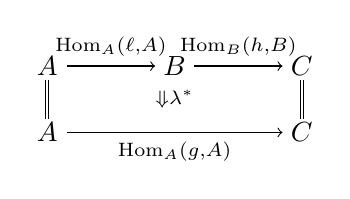
\begin{tikzpicture}[x=1em,y=1em]
  \node at (0,1.2)    {$A$};
  \node at (4.6,1.2)  {$B$};
  \node at (9.2,1.2)  {$C$};
  \node at (0,-1.2)   {$A$};
  \node at (9.2,-1.2) {$C$};
  \draw[->] (0.7,1.2)  -- node[above]{$\scriptstyle \mathrm{Hom}_{A}(\ell,A)$} (3.9,1.2);
  \draw[->] (5.3,1.2)  -- node[above]{$\scriptstyle \mathrm{Hom}_{B}(h,B)$} (8.5,1.2);
  \draw[->] (0.7,-1.2) -- node[below]{$\scriptstyle \mathrm{Hom}_{A}(g,A)$} (8.5,-1.2);
  \draw[double] (0,0.7)   -- (0,-0.7);
  \draw[double] (9.2,0.7) -- (9.2,-0.7);
  \node at (4.6,0) {$\scriptstyle\Downarrow\lambda^{*}$};
\end{tikzpicture}
\end{center}
在模的\trVirtualEquipment{}中定义一个右提升，则 $\lambda\colon g\Rightarrow \ell h$
是\trHomotopyTwoCategory{}中的一个左扩张。
\end{lemma}

\begin{proof}
由推论 8.4.9，二元\trCell{} $\nu_{*}\colon \mathrm{Hom}_{B}(B,k)\divideontimes\mathrm{Hom}_{C}(C,r)\Rightarrow \mathrm{Hom}_{C}(C,f)$ 对应于一元\trCell{}
$\nu_{*}\colon \mathrm{Hom}_{C}(C,rk)\Rightarrow \mathrm{Hom}_{C}(C,f)$；再由
命题 8.4.11，后者对应于\trHomotopyTwoCategory{}中的\trNaturalTransformation{}
$\nu\colon rk\Rightarrow f$。
在这一对应之下，限制到右可表示模时，\cref{def:right-extension-lifting-modules}
的泛性质显然涵盖了\cref{def:two-categorical-extension}的泛性质。
左扩张情形类似，经由定义 8.4.12 的反变嵌入。
\end{proof}

对于共变嵌入之像中的模右扩张图表，一个更精细的刻画出现在定理 9.3.3 中；但共变
嵌入之像中的模右提升图表，我们现在就能刻画。
请回忆定义 2.3.5 中引入的绝对右提升图表概念。

\begin{proposition}\label{prop:absolute-vs-module-lifting}
\trInfinityCosmos{}的\trHomotopyTwoCategory{}中如下左图所示的一个%
\trNaturalTransformation{}定义一个绝对右提升图表，当且仅当如下右图所示的那个
对应的二元\trCell{}在模的\trVirtualEquipment{}中定义一个右提升：
\begin{center}
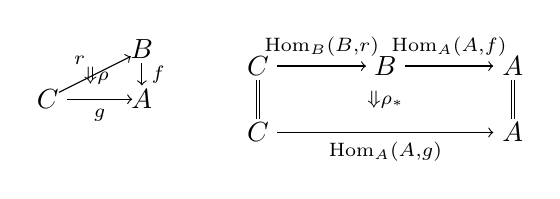
\begin{tikzpicture}[x=1em,y=1em]
  \node at (0,0)     {$C$};
  \node at (3.4,1.8) {$B$};
  \node at (3.4,0)   {$A$};
  \draw[->] (0.4,0.25) -- node[above left,pos=0.5]{$\scriptstyle r$} (3.0,1.55);
  \draw[->] (3.4,1.3)  -- node[right]{$\scriptstyle f$} (3.4,0.5);
  \draw[->] (0.7,0)    -- node[below]{$\scriptstyle g$} (3.05,0);
  \node at (1.75,0.85) {$\scriptstyle\Downarrow\rho$};
  \node at (5.9,0.85)  {$\leftrightsquigarrow$};
  \begin{scope}[shift={(7.6,0)}]
    \node at (0,1.2)    {$C$};
    \node at (4.6,1.2)  {$B$};
    \node at (9.2,1.2)  {$A$};
    \node at (0,-1.2)   {$C$};
    \node at (9.2,-1.2) {$A$};
    \draw[->] (0.7,1.2)  -- node[above]{$\scriptstyle \mathrm{Hom}_{B}(B,r)$} (3.9,1.2);
    \draw[->] (5.3,1.2)  -- node[above]{$\scriptstyle \mathrm{Hom}_{A}(A,f)$} (8.5,1.2);
    \draw[->] (0.7,-1.2) -- node[below]{$\scriptstyle \mathrm{Hom}_{A}(A,g)$} (8.5,-1.2);
    \draw[double] (0,0.7)   -- (0,-0.7);
    \draw[double] (9.2,0.7) -- (9.2,-0.7);
    \node at (4.6,0) {$\scriptstyle\Downarrow\rho_{*}$};
  \end{scope}
\end{tikzpicture}
\end{center}
对偶地，\trInfinityCosmos{}的\trHomotopyTwoCategory{}中如下左图所示的一个
2-\trCell{}定义一个绝对左提升图表，当且仅当如下右图所示的那个对应的二元%
\trCell{}在模的\trVirtualEquipment{}中定义一个右扩张：\footnote{原书印作
「$A$」，按模方向的型算应为 $C$，此处径改。——译者注}
\begin{center}
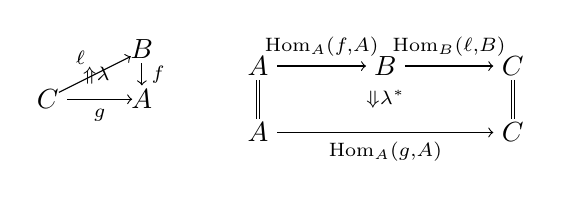
\begin{tikzpicture}[x=1em,y=1em]
  \node at (0,0)     {$C$};
  \node at (3.4,1.8) {$B$};
  \node at (3.4,0)   {$A$};
  \draw[->] (0.4,0.25) -- node[above left,pos=0.5]{$\scriptstyle\ell$} (3.0,1.55);
  \draw[->] (3.4,1.3)  -- node[right]{$\scriptstyle f$} (3.4,0.5);
  \draw[->] (0.7,0)    -- node[below]{$\scriptstyle g$} (3.05,0);
  \node at (1.75,0.85) {$\scriptstyle\Uparrow\lambda$};
  \node at (5.9,0.85)  {$\leftrightsquigarrow$};
  \begin{scope}[shift={(7.6,0)}]
    \node at (0,1.2)    {$A$};
    \node at (4.6,1.2)  {$B$};
    \node at (9.2,1.2)  {$C$};
    \node at (0,-1.2)   {$A$};
    \node at (9.2,-1.2) {$C$};
    \draw[->] (0.7,1.2)  -- node[above]{$\scriptstyle \mathrm{Hom}_{A}(f,A)$} (3.9,1.2);
    \draw[->] (5.3,1.2)  -- node[above]{$\scriptstyle \mathrm{Hom}_{B}(\ell,B)$} (8.5,1.2);
    \draw[->] (0.7,-1.2) -- node[below]{$\scriptstyle \mathrm{Hom}_{A}(g,A)$} (8.5,-1.2);
    \draw[double] (0,0.7)   -- (0,-0.7);
    \draw[double] (9.2,0.7) -- (9.2,-0.7);
    \node at (4.6,0) {$\scriptstyle\Downarrow\lambda^{*}$};
  \end{scope}
\end{tikzpicture}
\end{center}
\end{proposition}

\begin{proof}
由命题 8.4.11，\trInfinityCosmos{}的\trHomotopyTwoCategory{}中的诸%
\trNaturalTransformation{}与模的\trVirtualEquipment{}中各种形状的一元方块
一一对应。
由这一结果以及推论 8.4.6 与推论 8.4.9，存在诸典范双射：
\begin{rveq}\label{eq:canonical-bijections}
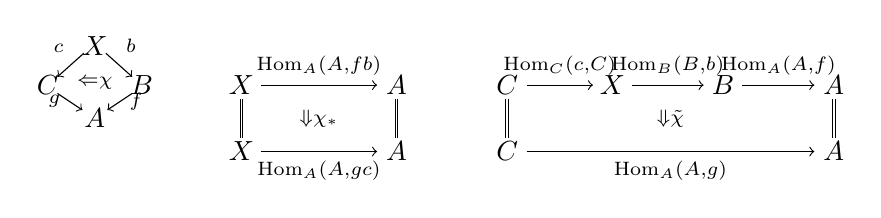
\begin{tikzpicture}[x=1em,y=1em]
  \node at (1.7,2.6) {$X$};
  \node at (0,1.2)   {$C$};
  \node at (3.4,1.2) {$B$};
  \node at (1.7,0)   {$A$};
  \draw[->] (2.1,2.35) -- node[above right,pos=0.4]{$\scriptstyle b$} (3.05,1.5);
  \draw[->] (1.3,2.35) -- node[above left,pos=0.4]{$\scriptstyle c$} (0.35,1.5);
  \draw[->] (3.05,0.9) -- node[right,pos=0.5]{$\scriptstyle f$} (2.15,0.3);
  \draw[->] (0.35,0.9) -- node[left,pos=0.5]{$\scriptstyle g$} (1.25,0.3);
  \node at (1.7,1.25) {$\scriptstyle\Leftarrow\chi$};
  \node at (5.3,1.2)  {$\leftrightsquigarrow$};
  \begin{scope}[shift={(7.0,0)}]
    \node at (0,1.2)    {$X$};
    \node at (5.6,1.2)  {$A$};
    \node at (0,-1.2)   {$X$};
    \node at (5.6,-1.2) {$A$};
    \draw[->] (0.7,1.2)  -- node[above]{$\scriptstyle \mathrm{Hom}_{A}(A,fb)$} (4.9,1.2);
    \draw[->] (0.7,-1.2) -- node[below]{$\scriptstyle \mathrm{Hom}_{A}(A,gc)$} (4.9,-1.2);
    \draw[double] (0,0.7)   -- (0,-0.7);
    \draw[double] (5.6,0.7) -- (5.6,-0.7);
    \node at (2.8,0) {$\scriptstyle\Downarrow\chi_{*}$};
  \end{scope}
  \node at (14.6,1.2) {$\leftrightsquigarrow$};
  \begin{scope}[shift={(16.6,0)}]
    \node at (0,1.2)    {$C$};
    \node at (3.8,1.2)  {$X$};
    \node at (7.8,1.2)  {$B$};
    \node at (11.8,1.2) {$A$};
    \node at (0,-1.2)   {$C$};
    \node at (11.8,-1.2){$A$};
    \draw[->] (0.7,1.2)  -- node[above]{$\scriptstyle \mathrm{Hom}_{C}(c,C)$} (3.1,1.2);
    \draw[->] (4.5,1.2)  -- node[above]{$\scriptstyle \mathrm{Hom}_{B}(B,b)$} (7.1,1.2);
    \draw[->] (8.5,1.2)  -- node[above]{$\scriptstyle \mathrm{Hom}_{A}(A,f)$} (11.1,1.2);
    \draw[->] (0.7,-1.2) -- node[below]{$\scriptstyle \mathrm{Hom}_{A}(A,g)$} (11.1,-1.2);
    \draw[double] (0,0.7)    -- (0,-0.7);
    \draw[double] (11.8,0.7) -- (11.8,-0.7);
    \node at (5.9,0) {$\scriptstyle\Downarrow\tilde{\chi}$};
  \end{scope}
\end{tikzpicture}
\end{rveq}

若二元\trCell{} $\rho_{*}\colon \mathrm{Hom}_{B}(B,r)\divideontimes\mathrm{Hom}_{A}(A,f)\Rightarrow \mathrm{Hom}_{A}(A,g)$ 在模的%
\trVirtualEquipment{}中定义一个右提升图表，则存在唯一的分解
\begin{center}
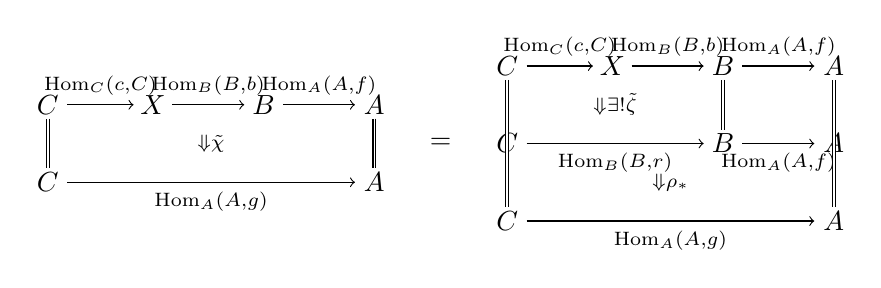
\begin{tikzpicture}[x=1em,y=1em]
  \begin{scope}
    \node at (0,1.4)    {$C$};
    \node at (3.8,1.4)  {$X$};
    \node at (7.8,1.4)  {$B$};
    \node at (11.8,1.4) {$A$};
    \node at (0,-1.4)   {$C$};
    \node at (11.8,-1.4){$A$};
    \draw[->] (0.7,1.4)  -- node[above]{$\scriptstyle \mathrm{Hom}_{C}(c,C)$} (3.1,1.4);
    \draw[->] (4.5,1.4)  -- node[above]{$\scriptstyle \mathrm{Hom}_{B}(B,b)$} (7.1,1.4);
    \draw[->] (8.5,1.4)  -- node[above]{$\scriptstyle \mathrm{Hom}_{A}(A,f)$} (11.1,1.4);
    \draw[->] (0.7,-1.4) -- node[below]{$\scriptstyle \mathrm{Hom}_{A}(A,g)$} (11.1,-1.4);
    \draw[double] (0,0.9)    -- (0,-0.9);
    \draw[double] (11.8,0.9) -- (11.8,-0.9);
    \node at (5.9,0) {$\scriptstyle\Downarrow\tilde{\chi}$};
  \end{scope}
  \node at (14.2,0) {$=$};
  \begin{scope}[shift={(16.6,0)}]
    \node at (0,2.8)    {$C$};
    \node at (3.8,2.8)  {$X$};
    \node at (7.8,2.8)  {$B$};
    \node at (11.8,2.8) {$A$};
    \draw[->] (0.7,2.8)  -- node[above]{$\scriptstyle \mathrm{Hom}_{C}(c,C)$} (3.1,2.8);
    \draw[->] (4.5,2.8)  -- node[above]{$\scriptstyle \mathrm{Hom}_{B}(B,b)$} (7.1,2.8);
    \draw[->] (8.5,2.8)  -- node[above]{$\scriptstyle \mathrm{Hom}_{A}(A,f)$} (11.1,2.8);
    \node at (0,0)    {$C$};
    \node at (7.8,0)  {$B$};
    \node at (11.8,0) {$A$};
    \draw[->] (0.7,0) -- node[below]{$\scriptstyle \mathrm{Hom}_{B}(B,r)$} (7.1,0);
    \draw[->] (8.5,0) -- node[below]{$\scriptstyle \mathrm{Hom}_{A}(A,f)$} (11.1,0);
    \node at (0,-2.8)   {$C$};
    \node at (11.8,-2.8){$A$};
    \draw[->] (0.7,-2.8) -- node[below]{$\scriptstyle \mathrm{Hom}_{A}(A,g)$} (11.1,-2.8);
    \draw[double] (0,2.3)    -- (0,-2.3);
    \draw[double] (11.8,2.3) -- (11.8,-2.3);
    \draw[double] (7.8,2.3)  -- (7.8,0.5);
    \node at (3.9,1.4)  {$\scriptstyle\Downarrow\exists!\tilde{\zeta}$};
    \node at (5.9,-1.4) {$\scriptstyle\Downarrow\rho_{*}$};
  \end{scope}
\end{tikzpicture}
\end{center}
反转 \eqref{eq:canonical-bijections} 的典范双射，这就定义了%
\trHomotopyTwoCategory{}中所要的那个唯一分解：
\begin{center}
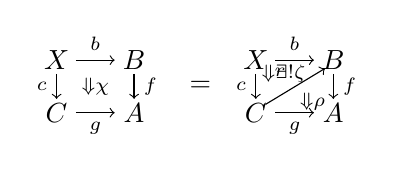
\begin{tikzpicture}[x=1em,y=1em]
  \node at (0,1.9)   {$X$};
  \node at (2.8,1.9) {$B$};
  \node at (0,0)     {$C$};
  \node at (2.8,0)   {$A$};
  \draw[->] (0.7,1.9) -- node[above]{$\scriptstyle b$} (2.1,1.9);
  \draw[->] (0,1.4)   -- node[left]{$\scriptstyle c$} (0,0.5);
  \draw[->] (2.8,1.4) -- node[right]{$\scriptstyle f$} (2.8,0.5);
  \draw[->] (0.7,0)   -- node[below]{$\scriptstyle g$} (2.1,0);
  \node at (1.4,0.95) {$\scriptstyle\Downarrow\chi$};
  \node at (5.2,0.95) {$=$};
  \begin{scope}[shift={(7.2,0)}]
    \node at (0,1.9)   {$X$};
    \node at (2.8,1.9) {$B$};
    \node at (0,0)     {$C$};
    \node at (2.8,0)   {$A$};
    \draw[->] (0.7,1.9) -- node[above]{$\scriptstyle b$} (2.1,1.9);
    \draw[->] (0,1.4)   -- node[left]{$\scriptstyle c$} (0,0.5);
    \draw[->] (2.8,1.4) -- node[right]{$\scriptstyle f$} (2.8,0.5);
    \draw[->] (0.7,0)   -- node[below]{$\scriptstyle g$} (2.1,0);
    \draw[->] (0.35,0.3) -- node[above left,pos=0.5]{$\scriptstyle r$} (2.5,1.6);
    \node at (1.0,1.4)  {$\scriptstyle\Downarrow\exists!\zeta$};
    \node at (2.05,0.4) {$\scriptstyle\Downarrow\rho$};
  \end{scope}
\end{tikzpicture}
\end{center}
于是，若 $\rho_{*}\colon \mathrm{Hom}_{B}(B,r)\divideontimes \mathrm{Hom}_{A}(A,f)\Rightarrow \mathrm{Hom}_{A}(A,g)$ 是一个右提升，则 $\rho\colon fr\Rightarrow g$
是一个绝对右提升。

反之，设 $\rho\colon fr\Rightarrow g$ 是一个绝对右提升，并考虑模的%
\trVirtualEquipment{}中如下形状的一个\trCell{}：
\begin{center}
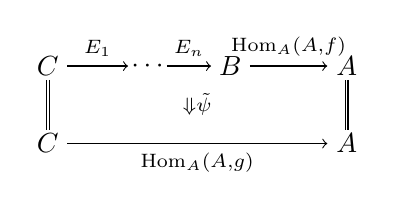
\begin{tikzpicture}[x=1em,y=1em]
  \node at (0,1.4)    {$C$};
  \node at (3.6,1.4)  {$\cdots$};
  \node at (6.6,1.4)  {$B$};
  \node at (10.8,1.4) {$A$};
  \node at (0,-1.4)   {$C$};
  \node at (10.8,-1.4){$A$};
  \draw[->] (0.7,1.4)  -- node[above]{$\scriptstyle E_{1}$} (2.9,1.4);
  \draw[->] (4.3,1.4)  -- node[above]{$\scriptstyle E_{n}$} (5.9,1.4);
  \draw[->] (7.3,1.4)  -- node[above]{$\scriptstyle \mathrm{Hom}_{A}(A,f)$} (10.1,1.4);
  \draw[->] (0.7,-1.4) -- node[below]{$\scriptstyle \mathrm{Hom}_{A}(A,g)$} (10.1,-1.4);
  \draw[double] (0,0.9)    -- (0,-0.9);
  \draw[double] (10.8,0.9) -- (10.8,-0.9);
  \node at (5.4,0) {$\scriptstyle\Downarrow\tilde{\psi}$};
\end{tikzpicture}
\end{center}
令 $C\overset{q}{\twoheadleftarrow}\vec{E}\overset{p}{\twoheadrightarrow}B$ 表示
复合双侧纤维化 $E_{1}\divideontimes\cdots\divideontimes E_{n}$。
由注 8.3.12，模映射 $\tilde{\psi}\colon E_{1}\divideontimes\cdots\divideontimes E_{n}\divideontimes\mathrm{Hom}_{A}(A,f)\Rightarrow \mathrm{Hom}_{A}(A,g)$ 对应于模映射
$\hat{\psi}\colon \mathrm{Hom}_{C}(q,C)\divideontimes \mathrm{Hom}_{B}(B,p)\divideontimes\mathrm{Hom}_{A}(A,f)\Rightarrow \mathrm{Hom}_{A}(A,g)$，如下左图所示。

如 \eqref{eq:canonical-bijections} 中所论，这些模映射与如下中图所示的诸%
\trNaturalTransformation{}处于一个典范双射之中：
\begin{center}
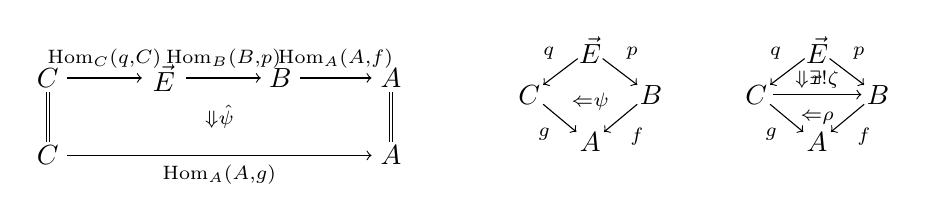
\begin{tikzpicture}[x=1em,y=1em]
  \begin{scope}
    \node at (0,1.4)    {$C$};
    \node at (4.2,1.4)  {$\vec{E}$};
    \node at (8.4,1.4)  {$B$};
    \node at (12.4,1.4) {$A$};
    \node at (0,-1.4)   {$C$};
    \node at (12.4,-1.4){$A$};
    \draw[->] (0.7,1.4)  -- node[above]{$\scriptstyle \mathrm{Hom}_{C}(q,C)$} (3.4,1.4);
    \draw[->] (5.0,1.4)  -- node[above]{$\scriptstyle \mathrm{Hom}_{B}(B,p)$} (7.7,1.4);
    \draw[->] (9.1,1.4)  -- node[above]{$\scriptstyle \mathrm{Hom}_{A}(A,f)$} (11.7,1.4);
    \draw[->] (0.7,-1.4) -- node[below]{$\scriptstyle \mathrm{Hom}_{A}(A,g)$} (11.7,-1.4);
    \draw[double] (0,0.9)    -- (0,-0.9);
    \draw[double] (12.4,0.9) -- (12.4,-0.9);
    \node at (6.2,0) {$\scriptstyle\Downarrow\hat{\psi}$};
  \end{scope}
  \node at (15.0,0) {$\leftrightsquigarrow$};
  \begin{scope}[shift={(17.4,0)}]
    \node at (2.2,2.4)  {$\vec{E}$};
    \node at (0,0.8)    {$C$};
    \node at (4.4,0.8)  {$B$};
    \node at (2.2,-0.9) {$A$};
    \draw[->] (1.75,2.1) -- node[above left,pos=0.4]{$\scriptstyle q$} (0.5,1.15);
    \draw[->] (2.65,2.1) -- node[above right,pos=0.4]{$\scriptstyle p$} (3.9,1.15);
    \draw[->] (0.5,0.45) -- node[below left,pos=0.5]{$\scriptstyle g$} (1.7,-0.55);
    \draw[->] (3.9,0.45) -- node[below right,pos=0.5]{$\scriptstyle f$} (2.7,-0.55);
    \node at (2.2,0.55) {$\scriptstyle\Leftarrow\psi$};
  \end{scope}
  \node at (23.2,0) {$\leftrightsquigarrow$};
  \begin{scope}[shift={(25.6,0)}]
    \node at (2.2,2.4)  {$\vec{E}$};
    \node at (0,0.8)    {$C$};
    \node at (4.4,0.8)  {$B$};
    \node at (2.2,-0.9) {$A$};
    \draw[->] (1.75,2.1) -- node[above left,pos=0.4]{$\scriptstyle q$} (0.5,1.15);
    \draw[->] (2.65,2.1) -- node[above right,pos=0.4]{$\scriptstyle p$} (3.9,1.15);
    \draw[->] (0.6,0.8)  -- node[above]{$\scriptstyle r$} (3.8,0.8);
    \draw[->] (0.5,0.45) -- node[below left,pos=0.5]{$\scriptstyle g$} (1.7,-0.55);
    \draw[->] (3.9,0.45) -- node[below right,pos=0.5]{$\scriptstyle f$} (2.7,-0.55);
    \node at (2.2,1.35)  {$\scriptstyle\Downarrow\exists!\zeta$};
    \node at (2.2,-0.05) {$\scriptstyle\Leftarrow\rho$};
  \end{scope}
\end{tikzpicture}
\end{center}
由于 $\rho\colon fr\Rightarrow g$ 被假定为绝对右提升，$\psi$ 经由 $\rho$ 唯一地
分解，从而如上右图那样定义了一个对应的 2-\trCell{} $\zeta\colon p\Rightarrow rq$。
再度应用 \eqref{eq:canonical-bijections}，这就构造出模的
\trVirtualEquipment{}中的一个唯一分解
\begin{center}
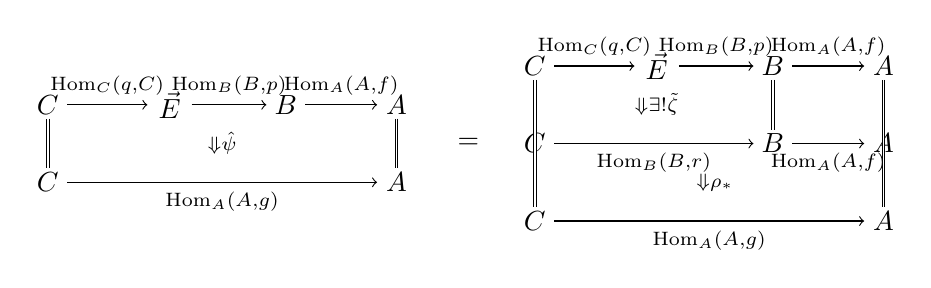
\begin{tikzpicture}[x=1em,y=1em]
  \begin{scope}
    \node at (0,1.4)    {$C$};
    \node at (4.4,1.4)  {$\vec{E}$};
    \node at (8.6,1.4)  {$B$};
    \node at (12.6,1.4) {$A$};
    \node at (0,-1.4)   {$C$};
    \node at (12.6,-1.4){$A$};
    \draw[->] (0.7,1.4)  -- node[above]{$\scriptstyle \mathrm{Hom}_{C}(q,C)$} (3.6,1.4);
    \draw[->] (5.2,1.4)  -- node[above]{$\scriptstyle \mathrm{Hom}_{B}(B,p)$} (7.9,1.4);
    \draw[->] (9.3,1.4)  -- node[above]{$\scriptstyle \mathrm{Hom}_{A}(A,f)$} (11.9,1.4);
    \draw[->] (0.7,-1.4) -- node[below]{$\scriptstyle \mathrm{Hom}_{A}(A,g)$} (11.9,-1.4);
    \draw[double] (0,0.9)    -- (0,-0.9);
    \draw[double] (12.6,0.9) -- (12.6,-0.9);
    \node at (6.3,0) {$\scriptstyle\Downarrow\hat{\psi}$};
  \end{scope}
  \node at (15.2,0) {$=$};
  \begin{scope}[shift={(17.6,0)}]
    \node at (0,2.8)    {$C$};
    \node at (4.4,2.8)  {$\vec{E}$};
    \node at (8.6,2.8)  {$B$};
    \node at (12.6,2.8) {$A$};
    \draw[->] (0.7,2.8)  -- node[above]{$\scriptstyle \mathrm{Hom}_{C}(q,C)$} (3.6,2.8);
    \draw[->] (5.2,2.8)  -- node[above]{$\scriptstyle \mathrm{Hom}_{B}(B,p)$} (7.9,2.8);
    \draw[->] (9.3,2.8)  -- node[above]{$\scriptstyle \mathrm{Hom}_{A}(A,f)$} (11.9,2.8);
    \node at (0,0)    {$C$};
    \node at (8.6,0)  {$B$};
    \node at (12.6,0) {$A$};
    \draw[->] (0.7,0) -- node[below]{$\scriptstyle \mathrm{Hom}_{B}(B,r)$} (7.9,0);
    \draw[->] (9.3,0) -- node[below]{$\scriptstyle \mathrm{Hom}_{A}(A,f)$} (11.9,0);
    \node at (0,-2.8)   {$C$};
    \node at (12.6,-2.8){$A$};
    \draw[->] (0.7,-2.8) -- node[below]{$\scriptstyle \mathrm{Hom}_{A}(A,g)$} (11.9,-2.8);
    \draw[double] (0,2.3)    -- (0,-2.3);
    \draw[double] (12.6,2.3) -- (12.6,-2.3);
    \draw[double] (8.6,2.3)  -- (8.6,0.5);
    \node at (4.4,1.4)  {$\scriptstyle\Downarrow\exists!\tilde{\zeta}$};
    \node at (6.5,-1.4) {$\scriptstyle\Downarrow\rho_{*}$};
  \end{scope}
\end{tikzpicture}
\end{center}
由注 8.3.12，这就定义了一个双射
\begin{center}
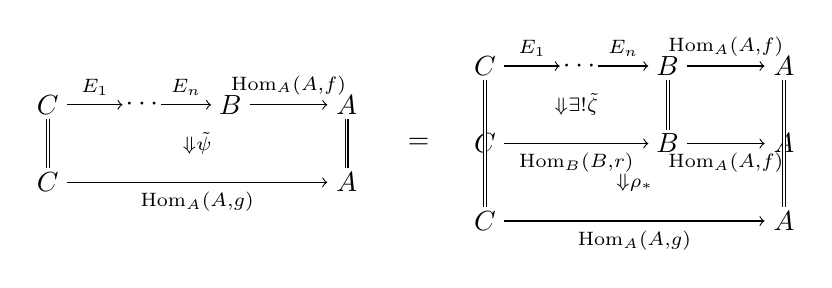
\begin{tikzpicture}[x=1em,y=1em]
  \begin{scope}
    \node at (0,1.4)    {$C$};
    \node at (3.4,1.4)  {$\cdots$};
    \node at (6.6,1.4)  {$B$};
    \node at (10.8,1.4) {$A$};
    \node at (0,-1.4)   {$C$};
    \node at (10.8,-1.4){$A$};
    \draw[->] (0.7,1.4)  -- node[above]{$\scriptstyle E_{1}$} (2.7,1.4);
    \draw[->] (4.1,1.4)  -- node[above]{$\scriptstyle E_{n}$} (5.9,1.4);
    \draw[->] (7.3,1.4)  -- node[above]{$\scriptstyle \mathrm{Hom}_{A}(A,f)$} (10.1,1.4);
    \draw[->] (0.7,-1.4) -- node[below]{$\scriptstyle \mathrm{Hom}_{A}(A,g)$} (10.1,-1.4);
    \draw[double] (0,0.9)    -- (0,-0.9);
    \draw[double] (10.8,0.9) -- (10.8,-0.9);
    \node at (5.4,0) {$\scriptstyle\Downarrow\tilde{\psi}$};
  \end{scope}
  \node at (13.4,0) {$=$};
  \begin{scope}[shift={(15.8,0)}]
    \node at (0,2.8)    {$C$};
    \node at (3.4,2.8)  {$\cdots$};
    \node at (6.6,2.8)  {$B$};
    \node at (10.8,2.8) {$A$};
    \draw[->] (0.7,2.8)  -- node[above]{$\scriptstyle E_{1}$} (2.7,2.8);
    \draw[->] (4.1,2.8)  -- node[above]{$\scriptstyle E_{n}$} (5.9,2.8);
    \draw[->] (7.3,2.8)  -- node[above]{$\scriptstyle \mathrm{Hom}_{A}(A,f)$} (10.1,2.8);
    \node at (0,0)    {$C$};
    \node at (6.6,0)  {$B$};
    \node at (10.8,0) {$A$};
    \draw[->] (0.7,0) -- node[below]{$\scriptstyle \mathrm{Hom}_{B}(B,r)$} (5.9,0);
    \draw[->] (7.3,0) -- node[below]{$\scriptstyle \mathrm{Hom}_{A}(A,f)$} (10.1,0);
    \node at (0,-2.8)   {$C$};
    \node at (10.8,-2.8){$A$};
    \draw[->] (0.7,-2.8) -- node[below]{$\scriptstyle \mathrm{Hom}_{A}(A,g)$} (10.1,-2.8);
    \draw[double] (0,2.3)    -- (0,-2.3);
    \draw[double] (10.8,2.3) -- (10.8,-2.3);
    \draw[double] (6.6,2.3)  -- (6.6,0.5);
    \node at (3.3,1.4)  {$\scriptstyle\Downarrow\exists!\tilde{\zeta}$};
    \node at (5.4,-1.4) {$\scriptstyle\Downarrow\rho_{*}$};
  \end{scope}
\end{tikzpicture}
\end{center}
于是，若 $\rho\colon fr\Rightarrow g$ 定义一个绝对右提升，则
$\rho_{*}\colon\mathrm{Hom}_{B}(B,r)\divideontimes \mathrm{Hom}_{A}(A,f)\Rightarrow\mathrm{Hom}_{A}(A,g)$
定义一个右提升。
\end{proof}

在定理 9.3.3 中我们将发现：共变嵌入之像中的那些模的右扩张，恰由%
\trHomotopyTwoCategory{}中所寻求的\emph{逐点}右扩张来刻画；对偶地，逐点左
扩张对应于反变嵌入之像中的那些模的右提升。在下一节中，我们将为这一概念的
2-范畴式定义逐步搭建基础。

\subsection*{练习}

\begin{exercise}\label{ex:uniqueness-right-extensions}
设 $B\xrightarrow{R}C$ 与 $B\xrightarrow{S}C$ 在\cref{def:right-extension-lifting-modules}
的意义下都定义了模 $A\xrightarrow{F}C$ 沿模 $A\xrightarrow{K}B$ 的一个右扩张。
请证明 $R\simeq_{B\times C}S$。
\end{exercise}

\begin{exercise}\label{ex:hom-cell-universal-properties}
不借助\cref{lem:canonical-restriction-cells}而完成\cref{lem:hom-binary-cell}
的证明。
\end{exercise}

\begin{exercise}\label{ex:closed-virtual-equipment}
一个\trVirtualEquipment{}是\textbf{封闭的}（closed），若\cref{def:right-extension-lifting-modules}
的右扩张与右提升总是存在。
在一个封闭\trVirtualEquipment{}中，请证明：一个\trCell{}
$\mu\colon E_{1}\divideontimes\cdots\divideontimes E_{n}\Rightarrow E$ 是一个复合，当且仅当沿 $\mu$ 的
限制对所有与 $E$ 平行的模 $F$ 都在纤维化一元\trCell{} $E\Rightarrow F$ 与
纤维化\trCell{} $E_{1}\divideontimes\cdots\divideontimes E_{n}\Rightarrow F$ 之间定义一个
双射。
\end{exercise}

\begin{exercise}\label{ex:right-liftings-through-composite}
将\cref{prop:right-extension-associativity}对偶化，以刻画穿过两支模之复合的
右提升。
\end{exercise}

\begin{exercise}\label{ex:dual-absolute-left-lifting}
建立\cref{prop:absolute-vs-module-lifting}的对偶：验证绝对左提升图表
$\lambda\colon g\Rightarrow f\ell$ 对应于右扩张图表
$\lambda^{*}\colon\mathrm{Hom}_{A}(f,A)\divideontimes \mathrm{Hom}_{B}(\ell,B)\Rightarrow\mathrm{Hom}_{A}(g,A)$。
\end{exercise}

   %
\providecommand{\HomA}{\mathrm{Hom}_{A}}
\providecommand{\HomB}{\mathrm{Hom}_{B}}
\providecommand{\HomC}{\mathrm{Hom}_{C}}
\providecommand{\HomD}{\mathrm{Hom}_{D}}
\providecommand{\HomE}{\mathrm{Hom}_{E}}
\providecommand{\HomP}{\mathrm{Hom}_{P}}

\section{正合方块}\label{sec:exact-squares}

为了引出本节的主要定义，让我们试着通过考察一个我们已经理解的特例，来猜测\trInfinityCosmos{}中逐点右\trExtension{}的\trUniversalProperty{}。若外围的\trInfinityCosmos{}是\trCartesianClosed{}，则图表 $f\colon A\to\mathcal{C}$ 沿函子 $k\colon A\to B$ 的逐点右\trExtension{}意在定义「限制函子
$\mathrm{res}_{k}\colon\mathcal{C}^{B}\to\mathcal{C}^{A}$ 在\trElement{} $f\colon 1\to\mathcal{C}^{A}$ 处的\trRightAdjoint{}」之值，而这个\trRightAdjoint{}可能整体存在，也可能不然。对于沿函子 $!\colon A\to 1$ 的扩张情形，限制函子正是定义 2.3.2 中考察的常值图表函子
$\Delta\colon\mathcal{C}\to\mathcal{C}^{A}$，于是经由定义 2.3.8，我们可以把逐点右\trExtension{}理解为计算 $f$ 的\trLimit{}。下述引理描述了这一\trUniversalProperty{}的转置形式。

\begin{lemma}\label{lem:limit-transpose}
在\trCartesianClosed{}\trInfinityCosmos{}中，下左三角形是一个绝对右提升图表——它定义 $f$ 的极限\trElement{}与极限\trCone——当且仅当转置所得的下中三角形具有如下性质：对任何\trInfinityCategory{} $X$，下右的复合图表是一个右\trExtension{}图表。
\begin{center}
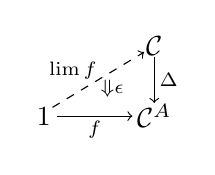
\begin{tikzpicture}[x=1.05em,y=1.05em]
  \node at (0,0) {$1$};
  \node at (3.8,0) {$\mathcal{C}^{A}$};
  \node at (3.8,2.4) {$\mathcal{C}$};
  \draw[->] (0.45,0) -- (3.05,0);
  \node at (1.75,-0.45) {$\scriptstyle f$};
  \draw[->] (3.8,2.05) -- (3.8,0.45);
  \node at (4.3,1.25) {$\scriptstyle\Delta$};
  \draw[->,dashed] (0.3,0.3) -- (3.45,2.2);
  \node at (1.0,1.55) {$\scriptstyle\lim f$};
  \node at (2.35,0.95) {$\scriptstyle\Downarrow\epsilon$};
\end{tikzpicture}
\qquad$\mathrel{\leftrightsquigarrow}$\qquad
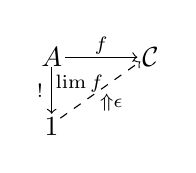
\begin{tikzpicture}[x=1.05em,y=1.05em]
  \node at (0,2.4) {$A$};
  \node at (3.4,2.4) {$\mathcal{C}$};
  \node at (0,0) {$1$};
  \draw[->] (0.45,2.4) -- (2.95,2.4);
  \node at (1.7,2.8) {$\scriptstyle f$};
  \draw[->] (0,2.05) -- (0,0.45);
  \node at (-0.4,1.25) {$\scriptstyle !$};
  \draw[->,dashed] (0.3,0.3) -- (3.05,2.25);
  \node at (0.95,1.5) {$\scriptstyle\lim f$};
  \node at (2.05,0.85) {$\scriptstyle\Uparrow\epsilon$};
\end{tikzpicture}
\qquad
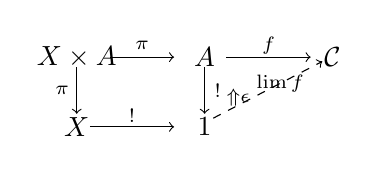
\begin{tikzpicture}[x=1.05em,y=1.05em]
  \node at (0,2.4) {$X\times A$};
  \node at (4.4,2.4) {$A$};
  \node at (8.8,2.4) {$\mathcal{C}$};
  \node at (0,0) {$X$};
  \node at (4.4,0) {$1$};
  \draw[->] (1.15,2.4) -- (3.35,2.4);
  \node at (2.25,2.8) {$\scriptstyle\pi$};
  \draw[->] (5.15,2.4) -- (8.05,2.4);
  \node at (6.6,2.8) {$\scriptstyle f$};
  \draw[->] (0,2.05) -- (0,0.45);
  \node at (-0.5,1.25) {$\scriptstyle\pi$};
  \node at (0.85,1.9) {$\scriptstyle\lrcorner$};
  \draw[->] (4.4,2.05) -- (4.4,0.45);
  \node at (4.85,1.25) {$\scriptstyle !$};
  \draw[->] (0.45,0) -- (3.35,0);
  \node at (1.9,0.38) {$\scriptstyle !$};
  \draw[->,dashed] (4.7,0.3) -- (8.45,2.25);
  \node at (7.0,1.5) {$\scriptstyle\lim f$};
  \node at (5.55,1.0) {$\scriptstyle\Uparrow\epsilon$};
\end{tikzpicture}
\end{center}
\end{lemma}

\begin{proof}
顶点为 $X$ 的一个\trCone{}经由 $f$ 沿常值图表函子的绝对右提升所得的因子分解
\begin{center}
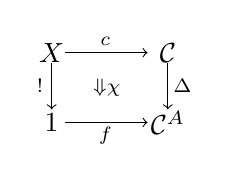
\begin{tikzpicture}[x=1.05em,y=1.05em]
  \node at (0,2.4) {$X$};
  \node at (4.0,2.4) {$\mathcal{C}$};
  \node at (0,0) {$1$};
  \node at (4.0,0) {$\mathcal{C}^{A}$};
  \draw[->] (0.45,2.4) -- (3.3,2.4);
  \node at (1.85,2.8) {$\scriptstyle c$};
  \draw[->] (0,2.05) -- (0,0.45);
  \node at (-0.4,1.25) {$\scriptstyle !$};
  \draw[->] (0.45,0) -- (3.3,0);
  \node at (1.85,-0.45) {$\scriptstyle f$};
  \draw[->] (4.0,2.05) -- (4.0,0.45);
  \node at (4.5,1.25) {$\scriptstyle\Delta$};
  \node at (1.9,1.2) {$\scriptstyle\Downarrow\chi$};
\end{tikzpicture}
\qquad$=$\qquad
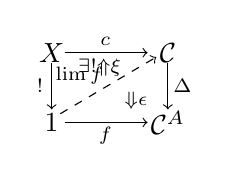
\begin{tikzpicture}[x=1.05em,y=1.05em]
  \node at (0,2.4) {$X$};
  \node at (4.0,2.4) {$\mathcal{C}$};
  \node at (0,0) {$1$};
  \node at (4.0,0) {$\mathcal{C}^{A}$};
  \draw[->] (0.45,2.4) -- (3.3,2.4);
  \node at (1.85,2.8) {$\scriptstyle c$};
  \draw[->] (0,2.05) -- (0,0.45);
  \node at (-0.4,1.25) {$\scriptstyle !$};
  \draw[->] (0.45,0) -- (3.3,0);
  \node at (1.85,-0.45) {$\scriptstyle f$};
  \draw[->] (4.0,2.05) -- (4.0,0.45);
  \node at (4.5,1.25) {$\scriptstyle\Delta$};
  \draw[->,dashed] (0.3,0.3) -- (3.6,2.25);
  \node at (0.95,1.6) {$\scriptstyle\lim f$};
  \node at (2.9,0.75) {$\scriptstyle\Downarrow\epsilon$};
  \node at (1.65,1.9) {$\scriptstyle\exists!\Uparrow\xi$};
\end{tikzpicture}
\end{center}
转置为如下因子分解：
\begin{center}
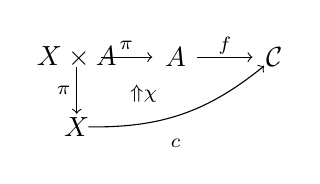
\begin{tikzpicture}[x=1.05em,y=1.05em]
  \node at (0,2.4) {$X\times A$};
  \node at (3.4,2.4) {$A$};
  \node at (6.8,2.4) {$\mathcal{C}$};
  \node at (0,0) {$X$};
  \draw[->] (0.85,2.4) -- (2.6,2.4);
  \node at (1.7,2.8) {$\scriptstyle\pi$};
  \draw[->] (4.15,2.4) -- (6.05,2.4);
  \node at (5.1,2.8) {$\scriptstyle f$};
  \draw[->] (0,2.05) -- (0,0.45);
  \node at (-0.45,1.25) {$\scriptstyle\pi$};
  \draw[->] (0.4,0) to[bend right=20] (6.45,2.1);
  \node at (3.4,-0.55) {$\scriptstyle c$};
  \node at (2.3,1.15) {$\scriptstyle\Uparrow\chi$};
\end{tikzpicture}
\qquad$=$\qquad
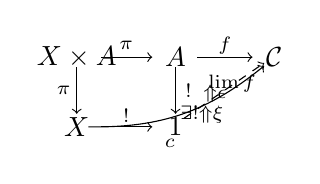
\begin{tikzpicture}[x=1.05em,y=1.05em]
  \node at (0,2.4) {$X\times A$};
  \node at (3.4,2.4) {$A$};
  \node at (6.8,2.4) {$\mathcal{C}$};
  \node at (0,0) {$X$};
  \node at (3.4,0) {$1$};
  \draw[->] (0.85,2.4) -- (2.6,2.4);
  \node at (1.7,2.8) {$\scriptstyle\pi$};
  \draw[->] (4.15,2.4) -- (6.05,2.4);
  \node at (5.1,2.8) {$\scriptstyle f$};
  \draw[->] (0,2.05) -- (0,0.45);
  \node at (-0.45,1.25) {$\scriptstyle\pi$};
  \node at (0.85,1.9) {$\scriptstyle\lrcorner$};
  \draw[->] (3.4,2.05) -- (3.4,0.45);
  \node at (3.85,1.25) {$\scriptstyle !$};
  \draw[->] (0.85,0) -- (2.6,0);
  \node at (1.7,0.38) {$\scriptstyle !$};
  \draw[->] (0.4,0) to[bend right=20] (6.45,2.1);
  \node at (3.2,-0.55) {$\scriptstyle c$};
  \draw[->,dashed] (3.7,0.3) -- (6.45,2.2);
  \node at (5.35,1.5) {$\scriptstyle\lim f$};
  \node at (4.75,1.15) {$\scriptstyle\Uparrow\epsilon$};
  \node at (4.3,0.42) {$\scriptstyle\exists!\Uparrow\xi$};
\end{tikzpicture}
\end{center}
\end{proof}

\cref{lem:limit-transpose}表明：要在一个未必\trCartesianClosed{}\trInfinityCosmos{}中定义 $f\colon A\to\mathcal{C}$ 的\trLimit{}，仅作出 $!\colon A\to 1$ 的右\trExtension{}是不够的。用定义 9.3.1 引入的术语来说，我们还须额外要求：该右\trExtension{}图表与如下形状的方块\emph{粘贴之后保持稳定}：
\begin{center}
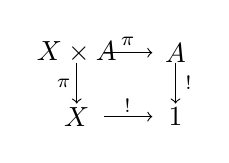
\begin{tikzpicture}[x=1.05em,y=1.05em]
  \node at (0,2.2) {$X\times A$};
  \node at (3.4,2.2) {$A$};
  \node at (0,0) {$X$};
  \node at (3.4,0) {$1$};
  \draw[->] (0.95,2.2) -- (2.6,2.2);
  \node at (1.75,2.6) {$\scriptstyle\pi$};
  \draw[->] (0,1.85) -- (0,0.45);
  \node at (-0.45,1.15) {$\scriptstyle\pi$};
  \node at (0.85,1.7) {$\scriptstyle\lrcorner$};
  \draw[->] (3.4,1.85) -- (3.4,0.45);
  \node at (3.85,1.15) {$\scriptstyle !$};
  \draw[->] (0.95,0) -- (2.6,0);
  \node at (1.75,0.38) {$\scriptstyle !$};
\end{tikzpicture}
\end{center}

我们该如何刻画这样的方块？首先，它们是每条腿都为\trBifibration{}的\trPullback{}。其次，它们是\trCommaSquare，其中\trCommaCone{}是一个恒同 $2$\trCell{}，其指向最好理解为与\cref{lem:limit-transpose}陈述中 $\epsilon$ 相容的方向。\footnote{原书印作「$\nu$」，而引理 9.2.1 全节的 2-胞腔记号为 $\epsilon$，疑为 $\epsilon$ 之误，此处径改。——译者注}由\cref{lem:comma-squares-exact}与\cref{lem:pullback-squares-exact}，我们将看到：这两者都是\emph{\trExactSquare{}}（exact square）的实例，我们现在即引入这一概念。

由命题 8.4.11，\trInfinityCosmos{}的\trHomotopyTwoCategory{}中的\trNaturalTransformation{}与模的\trVirtualEquipment{}中各种形状的一元方块一一对应；特别地，该结果与定理 8.4.4、命题 8.2.4 和命题 8.2.1 一起定义了一个\trCanonical{}双射：
\begin{center}
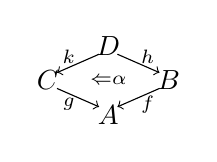
\begin{tikzpicture}[x=0.95em,y=0.95em]
  \node at (0,2.6) {$D$};
  \node at (-2.3,1.3) {$C$};
  \node at (2.3,1.3) {$B$};
  \node at (0,0) {$A$};
  \draw[->] (-0.35,2.3) -- (-1.95,1.6);
  \node at (-1.5,2.2) {$\scriptstyle k$};
  \draw[->] (0.35,2.3) -- (1.95,1.6);
  \node at (1.5,2.2) {$\scriptstyle h$};
  \draw[->] (-1.95,1.0) -- (-0.35,0.3);
  \node at (-1.5,0.4) {$\scriptstyle g$};
  \draw[->] (1.95,1.0) -- (0.35,0.3);
  \node at (1.5,0.4) {$\scriptstyle f$};
  \node at (0,1.3) {$\scriptstyle\Leftarrow\alpha$};
\end{tikzpicture}
\qquad$\mathrel{\leftrightsquigarrow}$\qquad
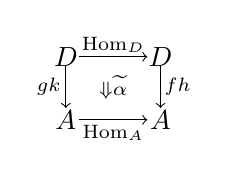
\begin{tikzpicture}[x=0.95em,y=0.95em]
  \node at (0,2.4) {$D$};
  \node at (3.6,2.4) {$D$};
  \node at (0,0) {$A$};
  \node at (3.6,0) {$A$};
  \draw[->] (0.5,2.4) -- (3.1,2.4);
  \node at (1.8,2.85) {$\scriptstyle\HomD$};
  \draw[->] (0.5,0) -- (3.1,0);
  \node at (1.8,-0.5) {$\scriptstyle\HomA$};
  \draw[->] (0,2.05) -- (0,0.45);
  \node at (-0.65,1.25) {$\scriptstyle gk$};
  \draw[->] (3.6,2.05) -- (3.6,0.45);
  \node at (4.25,1.25) {$\scriptstyle fh$};
  \node at (1.8,1.25) {$\scriptstyle\Downarrow\widetilde{\alpha}$};
\end{tikzpicture}
\qquad$\mathrel{\leftrightsquigarrow}$\qquad
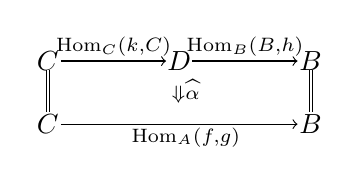
\begin{tikzpicture}[x=0.95em,y=0.95em]
  \node at (0,2.4) {$C$};
  \node at (5.0,2.4) {$D$};
  \node at (10.0,2.4) {$B$};
  \node at (0,0) {$C$};
  \node at (10.0,0) {$B$};
  \draw[->] (0.5,2.4) -- (4.5,2.4);
  \node at (2.5,2.95) {$\scriptstyle\HomC(k,C)$};
  \draw[->] (5.5,2.4) -- (9.5,2.4);
  \node at (7.5,2.95) {$\scriptstyle\HomB(B,h)$};
  \draw[double,double distance=0.6pt] (0,2.05) -- (0,0.45);
  \draw[double,double distance=0.6pt] (10.0,2.05) -- (10.0,0.45);
  \draw[->] (0.5,0) -- (9.5,0);
  \node at (5.25,-0.5) {$\scriptstyle\HomA(f,g)$};
  \node at (5.25,1.25) {$\scriptstyle\Downarrow\widehat{\alpha}$};
\end{tikzpicture}
\end{center}

\begin{definition}[\trExactSquare]\label{def:exact-square}
\trInfinityCosmos{}的\trHomotopyTwoCategory{}中的一个方块
\begin{center}
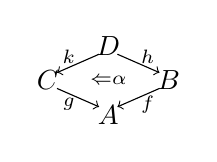
\begin{tikzpicture}[x=0.95em,y=0.95em]
  \node at (0,2.6) {$D$};
  \node at (-2.3,1.3) {$C$};
  \node at (2.3,1.3) {$B$};
  \node at (0,0) {$A$};
  \draw[->] (-0.35,2.3) -- (-1.95,1.6);
  \node at (-1.5,2.2) {$\scriptstyle k$};
  \draw[->] (0.35,2.3) -- (1.95,1.6);
  \node at (1.5,2.2) {$\scriptstyle h$};
  \draw[->] (-1.95,1.0) -- (-0.35,0.3);
  \node at (-1.5,0.4) {$\scriptstyle g$};
  \draw[->] (1.95,1.0) -- (0.35,0.3);
  \node at (1.5,0.4) {$\scriptstyle f$};
  \node at (0,1.3) {$\scriptstyle\Leftarrow\alpha$};
\end{tikzpicture}
\end{center}
是\textbf{正合的}\footnote{遗憾的是，「正合方块」这一术语在各种不同的场合都有使用。我们希望上下文足以表明，此处引入的概念与稳定\trInfinityCategory{}中既是推出又是拉回的方块毫无关系。练习 9.4.ii 揭示了这一正合方块概念与伴随函子之间对应为同构的交换方块二者之间的联系（见命题 6.3.10）。}%
，当且仅当左下所示的对应\trCell{}——它在引理 8.1.16 的双射之下编码为右下所示的粘贴复合
\begin{rveq}\label{eq:exact-square-cell}
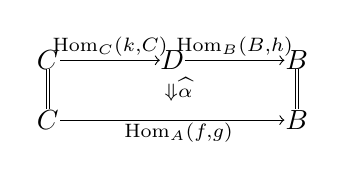
\begin{tikzpicture}[x=0.9em,y=0.9em]
  \node at (0,2.6) {$C$};
  \node at (5.0,2.6) {$D$};
  \node at (10.0,2.6) {$B$};
  \node at (0,0.2) {$C$};
  \node at (10.0,0.2) {$B$};
  \draw[->] (0.5,2.6) -- (4.5,2.6);
  \node at (2.5,3.15) {$\scriptstyle\HomC(k,C)$};
  \draw[->] (5.5,2.6) -- (9.5,2.6);
  \node at (7.5,3.15) {$\scriptstyle\HomB(B,h)$};
  \draw[double,double distance=0.6pt] (0,2.25) -- (0,0.65);
  \draw[double,double distance=0.6pt] (10.0,2.25) -- (10.0,0.65);
  \draw[->] (0.5,0.2) -- (9.5,0.2);
  \node at (5.25,-0.3) {$\scriptstyle\HomA(f,g)$};
  \node at (5.25,1.45) {$\scriptstyle\Downarrow\widehat{\alpha}$};
\end{tikzpicture}
\qquad\mathrel{\leftrightsquigarrow}\qquad
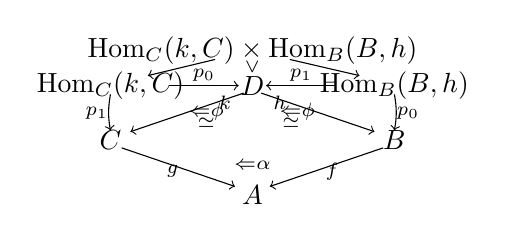
\begin{tikzpicture}[x=0.9em,y=0.9em]
  \node at (2.7,6.0) {$\HomC(k,C)\times\HomB(B,h)$};
  \node at (2.7,5.35) {$\scriptstyle\vee$};
  \draw[->] (1.2,5.65) -- (-1.5,5.0);
  \draw[->] (4.2,5.65) -- (7.0,5.0);
  \node at (-3.0,4.6) {$\HomC(k,C)$};
  \node at (2.7,4.6) {$D$};
  \node at (8.4,4.6) {$\HomB(B,h)$};
  \draw[->] (-0.65,4.6) -- (2.15,4.6);
  \node at (0.75,5.0) {$\scriptstyle p_{0}$};
  \draw[->] (6.05,4.6) -- (3.25,4.6);
  \node at (4.65,5.0) {$\scriptstyle p_{1}$};
  \draw[->] (-3.0,4.25) to[bend right=10] (-3.0,2.8);
  \node at (-3.55,3.5) {$\scriptstyle p_{1}$};
  \draw[->] (8.4,4.25) to[bend left=10] (8.4,2.8);
  \node at (8.95,3.5) {$\scriptstyle p_{0}$};
  \node at (0.85,3.55) {$\scriptstyle\Leftarrow\phi$};
  \node at (0.85,3.1) {$\scriptstyle\simeq$};
  \node at (4.5,3.55) {$\scriptstyle\Leftarrow\phi$};
  \node at (4.25,3.1) {$\scriptstyle\simeq$};
  \draw[->] (2.35,4.3) -- (-2.2,2.75);
  \node at (1.6,3.9) {$\scriptstyle k$};
  \draw[->] (3.05,4.3) -- (7.6,2.75);
  \node at (3.8,3.9) {$\scriptstyle h$};
  \node at (-3.0,2.4) {$C$};
  \node at (8.4,2.4) {$B$};
  \node at (2.7,0.2) {$A$};
  \draw[->] (-2.55,2.1) -- (2.0,0.55);
  \node at (-0.5,1.15) {$\scriptstyle g$};
  \draw[->] (7.95,2.1) -- (3.4,0.55);
  \node at (5.9,1.15) {$\scriptstyle f$};
  \node at (2.7,1.4) {$\scriptstyle\Leftarrow\alpha$};
\end{tikzpicture}
\end{rveq}
{\emergencystretch=6em
——把 $\HomA(f,g)$ 显示为定义 8.3.1 所定义意义下的复合
$\HomC(k,C)\otimes\HomB(B,h)$。\par}
\end{definition}

当边界方块在上下文中自明时，为节省语言，我们可以写「$\alpha\colon fh\Rightarrow gk$ 是一个正合方块」；但需注意，若被 $2$\trCell{} $\alpha$ 所栖居的方块的四条边界箭头中任何一条的位置发生移动，正合性条件的含义便会随之改变。\footnote{例如，比较\cref{lem:trivial-exact-squares}与引理 9.4.4 的陈述。}%

\begin{remark}[作为 Beck--Chevalley 条件的正合性]\label{rem:beck-chevalley}
由推论 8.4.8，由\trOneCellInduction{}所定义的如下\trSpan{}映射
\begin{center}
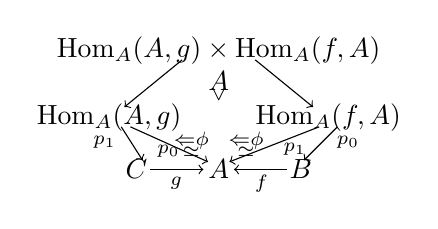
\begin{tikzpicture}[x=1.1em,y=1.1em]
  \node at (2.7,4.8) {$\HomA(A,g)\times\HomA(f,A)$};
  \node at (2.7,3.8) {$A$};
  \node at (2.7,3.35) {$\scriptstyle\vee$};
  \draw[->] (1.5,4.5) -- (-0.4,2.95);
  \draw[->] (3.9,4.5) -- (5.8,2.95);
  \node at (-0.9,2.6) {$\HomA(A,g)$};
  \node at (6.3,2.6) {$\HomA(f,A)$};
  \draw[->] (-0.5,2.3) -- (0.2,1.2);
  \node at (-1.05,1.8) {$\scriptstyle p_{1}$};
  \draw[->] (-0.2,2.3) -- (2.35,1.15);
  \node at (1.05,1.5) {$\scriptstyle p_{0}$};
  \draw[->] (6.0,2.3) -- (3.05,1.15);
  \node at (5.2,1.55) {$\scriptstyle p_{1}$};
  \draw[->] (6.6,2.3) -- (5.5,1.2);
  \node at (6.95,1.8) {$\scriptstyle p_{0}$};
  \node at (1.8,1.85) {$\scriptstyle\Leftarrow\phi$};
  \node at (1.8,1.47) {$\scriptstyle\simeq$};
  \node at (3.6,1.85) {$\scriptstyle\Leftarrow\phi$};
  \node at (3.6,1.47) {$\scriptstyle\simeq$};
  \node at (0,0.9) {$C$};
  \node at (2.7,0.9) {$A$};
  \node at (5.4,0.9) {$B$};
  \draw[->] (0.45,0.9) -- (2.2,0.9);
  \node at (1.3,0.45) {$\scriptstyle g$};
  \draw[->] (4.95,0.9) -- (3.2,0.9);
  \node at (4.1,0.45) {$\scriptstyle f$};
\end{tikzpicture}
\qquad$=$\qquad
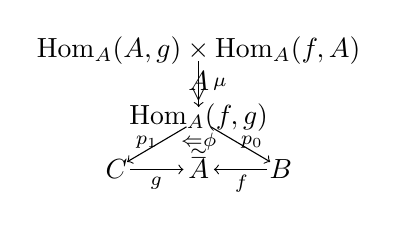
\begin{tikzpicture}[x=1.1em,y=1.1em]
  \node at (2.7,4.8) {$\HomA(A,g)\times\HomA(f,A)$};
  \node at (2.7,3.8) {$A$};
  \node at (2.7,3.35) {$\scriptstyle\vee$};
  \draw[->] (2.7,4.45) -- (2.7,2.95);
  \node at (3.4,3.7) {$\scriptstyle\ulcorner\mu\urcorner$};
  \node at (2.7,2.6) {$\HomA(f,g)$};
  \draw[->] (2.3,2.3) -- (0.35,1.15);
  \node at (1.0,1.8) {$\scriptstyle p_{1}$};
  \draw[->] (3.1,2.3) -- (5.05,1.15);
  \node at (4.45,1.8) {$\scriptstyle p_{0}$};
  \node at (2.7,1.8) {$\scriptstyle\Leftarrow\phi$};
  \node at (2.7,1.42) {$\scriptstyle\simeq$};
  \node at (0,0.9) {$C$};
  \node at (2.7,0.9) {$A$};
  \node at (5.4,0.9) {$B$};
  \draw[->] (0.45,0.9) -- (2.2,0.9);
  \node at (1.3,0.45) {$\scriptstyle g$};
  \draw[->] (4.95,0.9) -- (3.2,0.9);
  \node at (4.1,0.45) {$\scriptstyle f$};
\end{tikzpicture}
\end{center}
编码了一个二元\trCell{}
$\mu\colon\HomA(A,g)\divideontimes\HomA(f,A)\Rightarrow\HomA(f,g)$，它是一个复合。正合性说，$\alpha$ 诱导了从 $C$ 到 $B$ 的模的如下\trIsomorphism
\begin{equation*}
\widehat{\alpha}\colon\HomC(k,C)\otimes\HomB(B,h)\simeq\HomA(A,g)\otimes\HomA(f,A)
\end{equation*}
\end{remark}

\begin{digression}[强正合性]\label{dig:strong-exactness}
回忆 8.3 节：在任何\trVirtualEquipment{}中出现的许多形式地定义的复合\trCell{}，在与一个\trInfinityCosmos{}相联系的模的\trVirtualEquipment{}中实际上是强复合。基于这一经验，人们或许会预期：我们在模的\trVirtualEquipment{}中遇到的许多\trExactSquare{}实际上都是\textbf{强正合}的，意即\trCell{}
$\widehat{\alpha}\colon\HomC(k,C)\divideontimes\HomB(B,h)\Rightarrow\HomA(f,g)$ 是一个强复合——而事实也确实如此。事实上，在 $(\infty,1)$-范畴的\trInfinityCosmos{}中，所有复合都存在且都是强的：模的张量积可以通过一种对\trPullback{}稳定的逐纤维的余反转器（coinverter）构造来定义。由于模的任何相容序列的复合都等价于强复合，在这类\trInfinityCosmos{}中，所有复合、从而所有\trExactSquare{}都自动满足更强的\trUniversalProperty{}。

\trExactSquare{}在此处扮演的主要角色，是发展逐点左\trExtension{}与右\trExtension{}的概念；为此，较弱的 2-范畴性\trUniversalProperty{}已然足够。我们顺带指出：我们形式地定义的\trExactSquare{}都是强的，但在证明中我们通常只诉诸较弱的正合性质。仅有一种情形下更强的正合性概念可能更为妥当，我们将在注 9.4.12 中讨论它。
\end{digression}

本节的其余部分致力于\trExactSquare{}的例子。

\begin{lemma}[\trCommaSquare{}是正合的]\label{lem:comma-squares-exact}
对任何余跨度 $C\overset{g}{\to}A\overset{f}{\gets}B$，\trCommaCone{}定义了一个强正合方块：
\begin{center}
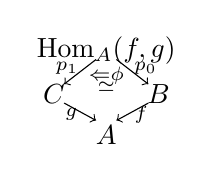
\begin{tikzpicture}[x=1.05em,y=1.05em]
  \node at (0,2.4) {$\HomA(f,g)$};
  \draw[->] (-0.35,2.1) -- (-1.45,1.25);
  \node at (-1.35,1.8) {$\scriptstyle p_{1}$};
  \draw[->] (0.35,2.1) -- (1.45,1.25);
  \node at (1.35,1.8) {$\scriptstyle p_{0}$};
  \node at (-1.8,0.9) {$C$};
  \node at (1.8,0.9) {$B$};
  \node at (0,1.55) {$\scriptstyle\Leftarrow\phi$};
  \node at (0,1.15) {$\scriptstyle\simeq$};
  \draw[->] (-1.45,0.6) -- (-0.35,0.0);
  \node at (-1.2,0.2) {$\scriptstyle g$};
  \draw[->] (1.45,0.6) -- (0.35,0.0);
  \node at (1.2,0.2) {$\scriptstyle f$};
  \node at (0,-0.5) {$A$};
\end{tikzpicture}
\end{center}
\end{lemma}

\begin{proof}
由命题 8.3.11，模 $C\xrightarrow{\HomA(f,g)}B$ 是其左腿的左表示后接其右腿的右表示而成的强复合。由注 8.3.13，二元复合\trCell{}
$\HomC(p_{1},C)\divideontimes\HomB(B,p_{0})\Rightarrow\HomA(f,g)$ 在引理 8.1.16 的双射之下对应于粘贴复合
\begin{center}
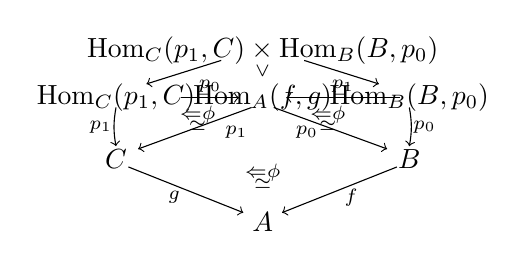
\begin{tikzpicture}[x=1.0em,y=1.0em]
  \node at (2.7,5.9) {$\HomC(p_{1},C)\times\HomB(B,p_{0})$};
  \node at (2.7,5.15) {$\scriptstyle\vee$};
  \draw[->] (1.2,5.55) -- (-1.5,4.7);
  \draw[->] (4.2,5.55) -- (6.9,4.7);
  \node at (-2.6,4.2) {$\HomC(p_{1},C)$};
  \node at (2.7,4.2) {$\HomA(f,g)$};
  \node at (8.0,4.2) {$\HomB(B,p_{0})$};
  \draw[->] (-0.25,4.2) -- (1.85,4.2);
  \node at (0.8,4.62) {$\scriptstyle p_{0}$};
  \draw[->] (7.65,4.2) -- (3.55,4.2);
  \node at (5.6,4.62) {$\scriptstyle p_{1}$};
  \draw[->] (-2.6,3.85) to[bend right=10] (-2.6,2.45);
  \node at (-3.15,3.15) {$\scriptstyle p_{1}$};
  \draw[->] (8.0,3.85) to[bend left=10] (8.0,2.45);
  \node at (8.55,3.15) {$\scriptstyle p_{0}$};
  \node at (0.35,3.6) {$\scriptstyle\Leftarrow\phi$};
  \node at (0.35,3.2) {$\scriptstyle\simeq$};
  \node at (5.05,3.6) {$\scriptstyle\Leftarrow\phi$};
  \node at (5.05,3.2) {$\scriptstyle\simeq$};
  \draw[->] (2.3,3.85) -- (-1.8,2.35);
  \node at (1.75,2.95) {$\scriptstyle p_{1}$};
  \draw[->] (3.1,3.85) -- (7.2,2.35);
  \node at (4.3,2.95) {$\scriptstyle p_{0}$};
  \node at (-2.6,2.0) {$C$};
  \node at (8.0,2.0) {$B$};
  \node at (2.7,1.5) {$\scriptstyle\Leftarrow\phi$};
  \node at (2.7,1.1) {$\scriptstyle\simeq$};
  \draw[->] (-2.15,1.7) -- (2.0,0.05);
  \node at (-0.5,0.6) {$\scriptstyle g$};
  \draw[->] (7.55,1.7) -- (3.4,0.05);
  \node at (5.9,0.6) {$\scriptstyle f$};
  \node at (2.7,-0.3) {$A$};
\end{tikzpicture}
\end{center}
这便恢复了由 \eqref{eq:exact-square-cell} 所定义的、检验\trCommaSquare
$\phi\colon fp_{0}\Rightarrow gp_{1}$ 正合性的胞腔 $\widehat{\phi}$。
\end{proof}

\begin{lemma}\label{lem:pullback-squares-exact}
若 $g\colon C\to A$ 是一个\trCartesianFibration{}或 $f\colon B\to A$ 是一个\trCocartesianFibration{}，则此\trPullback{}方块是强正合的：
\begin{center}
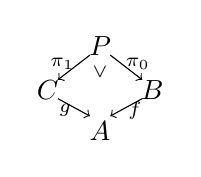
\begin{tikzpicture}[x=1.05em,y=1.05em]
  \node at (0,2.4) {$P$};
  \draw[->] (-0.35,2.1) -- (-1.45,1.25);
  \node at (-1.3,1.8) {$\scriptstyle\pi_{1}$};
  \node at (0,1.5) {$\scriptstyle\vee$};
  \draw[->] (0.35,2.1) -- (1.45,1.25);
  \node at (1.3,1.8) {$\scriptstyle\pi_{0}$};
  \node at (-1.8,0.9) {$C$};
  \node at (1.8,0.9) {$B$};
  \draw[->] (-1.45,0.6) -- (-0.35,0.0);
  \node at (-1.2,0.2) {$\scriptstyle g$};
  \draw[->] (1.45,0.6) -- (0.35,0.0);
  \node at (1.2,0.2) {$\scriptstyle f$};
  \node at (0,-0.5) {$A$};
\end{tikzpicture}
\end{center}
\end{lemma}

\begin{proof}
这两个断言是对偶的，不过——正如证明所揭示的——余笛卡尔纤维化与笛卡尔纤维化的位置不可互换。若 $f\colon B\to A$ 是一个\trCocartesianFibration{}，注意到：由恒同 $2$\trCell{} $f\pi_{0}=g\pi_{1}$ 诱导的函子 $\Delta\colon P\to\HomA(f,g)$，是由恒同 $2$\trCell{} $\mathrm{id}_{f}$ 诱导的函子 $\Delta_{f}\colon B\to\HomA(f,A)$ 的一个\trPullback{}：
\begin{center}
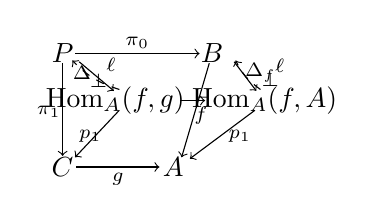
\begin{tikzpicture}[x=1.0em,y=1.0em]
  \node at (0,3.2) {$P$};
  \node at (5.4,3.2) {$B$};
  \draw[->] (0.45,3.2) -- (4.95,3.2);
  \node at (2.7,3.6) {$\scriptstyle\pi_{0}$};
  \draw[->] (0.6,2.9) -- (1.85,1.85);
  \node at (0.7,2.5) {$\scriptstyle\Delta$};
  \draw[->,dashed] (2.05,1.9) to[bend left=14] (0.35,2.95);
  \node at (1.75,2.8) {$\scriptstyle\ell$};
  \node at (1.3,2.2) {$\scriptstyle\perp$};
  \draw[->] (6.2,2.9) -- (7.0,1.85);
  \node at (7.15,2.5) {$\scriptstyle\Delta_{f}$};
  \draw[->,dashed] (7.15,1.9) to[bend left=14] (6.25,2.95);
  \node at (7.85,2.75) {$\scriptstyle\ell$};
  \node at (7.5,2.25) {$\scriptstyle\perp$};
  \node at (1.9,1.5) {$\HomA(f,g)$};
  \node at (7.3,1.5) {$\HomA(f,A)$};
  \draw[->] (4.25,1.5) -- (5.15,1.5);
  \node at (1.9,1.0) {$\scriptstyle\lrcorner$};
  \draw[->] (0,2.85) -- (0,-0.5);
  \node at (-0.5,1.1) {$\scriptstyle\pi_{1}$};
  \draw[->] (2.05,1.15) -- (0.45,-0.55);
  \node at (1.0,0.2) {$\scriptstyle p_{1}$};
  \draw[->] (5.3,2.85) -- (4.3,-0.55);
  \node at (5.0,0.95) {$\scriptstyle f$};
  \draw[->] (6.95,1.15) -- (4.6,-0.6);
  \node at (6.4,0.2) {$\scriptstyle p_{1}$};
  \node at (0,-0.9) {$C$};
  \node at (4.0,-0.9) {$A$};
  \draw[->] (0.5,-0.9) -- (3.5,-0.9);
  \node at (2.0,-1.35) {$\scriptstyle g$};
\end{tikzpicture}
\end{center}
由于 $f$ 是\trCocartesianFibration{}，定理 5.2.8(iii) 告诉我们：$\Delta_{f}\colon B\to\HomA(f,A)$ 在 $A$ 上带有一个\trFiberedAdjunction{}。这一\trFiberedAdjunction{}沿 $g\colon C\to A$ 作\trPullback{}之后，便给出 $\Delta\colon P\to\HomA(f,g)$ 的一个\trFiberedAdjunction{}。
由于 $\pi_{0}=p_{0}\Delta$，推论 8.4.9 蕴含：\trCanonical{}\trCell
\begin{equation*}
\begin{aligned}
&\mathrm{Hom}^{\HomA(f,g)}(\HomA(f,g),\Delta)\\
&\divideontimes\HomB(B,p_{0})\Rightarrow\HomB(B,\pi_{0})
\end{aligned}
\end{equation*}
{\emergencystretch=6em
是一个强复合。由于 $\ell\dashv\Delta$，由命题 4.1.1 存在\trEquivalence{}
$\HomP(\ell,P)\simeq\allowbreak\mathrm{Hom}_{\HomA(f,g)}(\HomA(f,g),\Delta)$。又由于 $p_{1}=\pi_{1}\ell$，由推论 8.4.9，\trCanonical{}\trCell
\begin{equation*}
\HomC(\pi_{1},C)\divideontimes\HomP(\ell,P)\Rightarrow\HomC(p_{1},C)
\end{equation*}}
是一个强复合。将这些双射复合起来，我们便看到：定义域为
$\HomC(\pi_{1},C)\divideontimes\HomB(B,\pi_{0})$ 的\trCell{}与定义域为
$\HomC(p_{1},C)\divideontimes\HomB(B,p_{0})$ 的\trCell{}之间一一对应。
由于 $\ell\dashv\Delta$ 是一个\trFiberedAdjunction{}，\trNaturalTransformation{}
$\phi\colon fp_{0}\Rightarrow gp_{1}=g\pi_{1}\ell$ 沿 $\ell\dashv\Delta$ 的转置等于
$\phi\Delta=\mathrm{id}\colon f\pi_{0}=fp_{0}i\Rightarrow gp_{1}i=g\pi_{1}$。这说明，如下两\trCell
\begin{equation*}
\begin{aligned}
\widehat{\mathrm{id}}&\colon\HomC(\pi_{1},C)\divideontimes\HomB(B,\pi_{0})\Rightarrow\HomA(f,g),\\
\widehat{\phi}&\colon\HomC(p_{1},C)\divideontimes\HomB(B,p_{0})\Rightarrow\HomA(f,g)
\end{aligned}
\end{equation*}
在刚刚描述的双射之下相互对应。由于\cref{lem:comma-squares-exact}证明了 $\widehat{\phi}$ 是一个强复合，由引理 8.3.8，$\widehat{\mathrm{id}}$ 亦然。
\end{proof}

为了后续使用，我们在此记录\trExactSquare{}的一些平凡例子。

\begin{lemma}\label{lem:trivial-exact-squares}
对任何一对函子 $k\colon A\to B$ 与 $h\colon C\to D$，\trPullback{}方块是强正合的：
\begin{center}
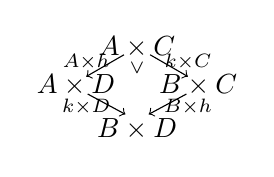
\begin{tikzpicture}[x=1.05em,y=1.05em]
  \node at (0,2.4) {$A\times C$};
  \draw[->] (-0.45,2.15) -- (-1.75,1.4);
  \node at (-1.75,1.9) {$\scriptstyle A\times h$};
  \node at (0,1.7) {$\scriptstyle\vee$};
  \draw[->] (0.45,2.15) -- (1.75,1.4);
  \node at (1.75,1.9) {$\scriptstyle k\times C$};
  \node at (-2.1,1.1) {$A\times D$};
  \node at (2.1,1.1) {$B\times C$};
  \draw[->] (-1.7,0.8) -- (-0.4,0.1);
  \node at (-1.75,0.35) {$\scriptstyle k\times D$};
  \draw[->] (1.7,0.8) -- (0.4,0.1);
  \node at (1.75,0.35) {$\scriptstyle B\times h$};
  \node at (0,-0.4) {$B\times D$};
\end{tikzpicture}
\end{center}
特别地，恒同\trCell{}定义强正合方块：
\begin{center}
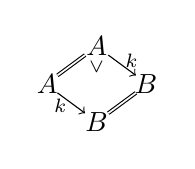
\begin{tikzpicture}[x=1.05em,y=1.05em]
  \node at (0,2.4) {$A$};
  \draw[double,double distance=0.6pt] (-0.4,2.1) -- (-1.35,1.4);
  \node at (0,1.7) {$\scriptstyle\vee$};
  \draw[->] (0.4,2.1) -- (1.35,1.4);
  \node at (1.2,1.9) {$\scriptstyle k$};
  \node at (-1.7,1.1) {$A$};
  \node at (1.7,1.1) {$B$};
  \draw[->] (-1.35,0.8) -- (-0.4,0.1);
  \node at (-1.25,0.35) {$\scriptstyle k$};
  \draw[double,double distance=0.6pt] (1.35,0.8) -- (0.4,0.1);
  \node at (0,-0.2) {$B$};
\end{tikzpicture}
\qquad
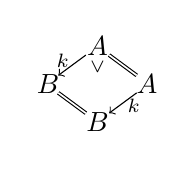
\begin{tikzpicture}[x=1.05em,y=1.05em]
  \node at (0,2.4) {$A$};
  \draw[->] (-0.4,2.1) -- (-1.35,1.4);
  \node at (-1.2,1.9) {$\scriptstyle k$};
  \node at (0,1.7) {$\scriptstyle\vee$};
  \draw[double,double distance=0.6pt] (0.4,2.1) -- (1.35,1.4);
  \node at (-1.7,1.1) {$B$};
  \node at (1.7,1.1) {$A$};
  \draw[double,double distance=0.6pt] (-1.35,0.8) -- (-0.4,0.1);
  \draw[->] (1.35,0.8) -- (0.4,0.1);
  \node at (1.25,0.35) {$\scriptstyle k$};
  \node at (0,-0.2) {$B$};
\end{tikzpicture}
\end{center}
\end{lemma}

\begin{proof}
\cref{ex:prove-trivial-exact-squares}。
\end{proof}

最后，刚刚建立的这些\trExactSquare{}还可以复合起来，产生进一步的\trExactSquare{}：

\begin{lemma}[正合方块的复合]\label{lem:composites-exact-squares}
给定\trHomotopyTwoCategory{}中如下图式所示的方块图表
\begin{center}
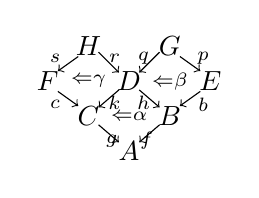
\begin{tikzpicture}[x=1.05em,y=1.05em]
  \node at (-1.4,2.9) {$H$};
  \node at (1.4,2.9) {$G$};
  \node at (-2.8,1.7) {$F$};
  \node at (0,1.7) {$D$};
  \node at (2.8,1.7) {$E$};
  \node at (-1.4,0.5) {$C$};
  \node at (1.4,0.5) {$B$};
  \node at (0,-0.7) {$A$};
  \draw[->] (-1.75,2.55) -- (-2.45,2.05);
  \node at (-2.55,2.5) {$\scriptstyle s$};
  \draw[->] (-1.05,2.7) -- (-0.35,2.0);
  \node at (-0.5,2.5) {$\scriptstyle r$};
  \draw[->] (1.05,2.7) -- (0.35,2.0);
  \node at (0.5,2.5) {$\scriptstyle q$};
  \draw[->] (1.75,2.55) -- (2.45,2.05);
  \node at (2.55,2.5) {$\scriptstyle p$};
  \draw[->] (-2.45,1.35) -- (-1.75,0.85);
  \node at (-2.55,0.9) {$\scriptstyle c$};
  \draw[->] (-0.35,1.4) -- (-1.05,0.8);
  \node at (-0.5,0.95) {$\scriptstyle k$};
  \draw[->] (0.35,1.4) -- (1.05,0.8);
  \node at (0.5,0.95) {$\scriptstyle h$};
  \draw[->] (2.45,1.35) -- (1.75,0.85);
  \node at (2.55,0.9) {$\scriptstyle b$};
  \draw[->] (-1.05,0.2) -- (-0.35,-0.4);
  \node at (-0.6,-0.35) {$\scriptstyle g$};
  \draw[->] (1.05,0.2) -- (0.35,-0.4);
  \node at (0.6,-0.35) {$\scriptstyle f$};
  \node at (-1.4,1.7) {$\scriptstyle\Leftarrow\gamma$};
  \node at (1.4,1.7) {$\scriptstyle\Leftarrow\beta$};
  \node at (0,0.5) {$\scriptstyle\Leftarrow\alpha$};
\end{tikzpicture}
\end{center}
若 $\alpha\colon fh\Rightarrow gk$、$\beta\colon bp\Rightarrow hq$ 与
$\gamma\colon kr\Rightarrow cs$ 都是正合方块，则复合矩形
$\alpha q\cdot f\beta$ 与 $g\gamma\cdot\alpha r$ 也是正合方块；且当构成它们的方块都强正合时，这两个矩形也强正合。由此，（强）正合方块的任意「\trDoubleCategory{}式」复合都定义（强）正合方块。
\end{lemma}

\begin{proof}
这两种情形互为余对偶，故只需证明矩形
$\alpha q\cdot f\beta\colon g(kq)\Rightarrow(fb)p$ 是正合的。对应的胞腔
$\widehat{\alpha q\cdot f\beta}$ 显示于下左，它经由复合 $\widehat{\beta}$ 在下右分解：
\begin{center}
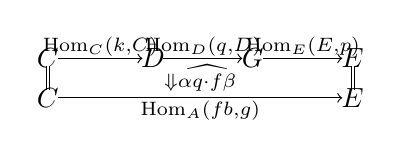
\begin{tikzpicture}[x=0.95em,y=0.95em]
  \node at (-4.6,1.2) {$C$};
  \node at (-0.6,1.2) {$D$};
  \node at (3.2,1.2) {$G$};
  \node at (7.0,1.2) {$E$};
  \draw[->] (-4.2,1.2) -- (-1.0,1.2);
  \node at (-2.6,1.65) {$\scriptstyle\HomC(k,C)$};
  \draw[->] (-0.2,1.2) -- (2.8,1.2);
  \node at (1.3,1.65) {$\scriptstyle\HomD(q,D)$};
  \draw[->] (3.6,1.2) -- (6.6,1.2);
  \node at (5.1,1.65) {$\scriptstyle\HomE(E,p)$};
  \draw[double,double distance=0.6pt] (-4.6,0.9) -- (-4.6,0.0);
  \draw[double,double distance=0.6pt] (7.0,0.9) -- (7.0,0.0);
  \node at (1.2,0.45) {$\scriptstyle\Downarrow\widehat{\alpha q\cdot f\beta}$};
  \node at (-4.6,-0.3) {$C$};
  \node at (7.0,-0.3) {$E$};
  \draw[->] (-4.2,-0.3) -- (6.6,-0.3);
  \node at (1.2,-0.8) {$\scriptstyle\HomA(fb,g)$};
\end{tikzpicture}
\qquad$=$\qquad
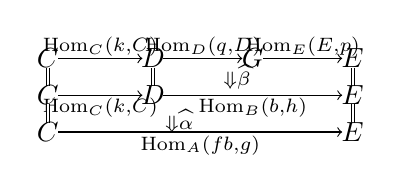
\begin{tikzpicture}[x=0.95em,y=0.95em]
  \node at (-4.6,2.3) {$C$};
  \node at (-0.6,2.3) {$D$};
  \node at (3.2,2.3) {$G$};
  \node at (7.0,2.3) {$E$};
  \draw[->] (-4.2,2.3) -- (-1.0,2.3);
  \node at (-2.6,2.75) {$\scriptstyle\HomC(k,C)$};
  \draw[->] (-0.2,2.3) -- (2.8,2.3);
  \node at (1.3,2.75) {$\scriptstyle\HomD(q,D)$};
  \draw[->] (3.6,2.3) -- (6.6,2.3);
  \node at (5.1,2.75) {$\scriptstyle\HomE(E,p)$};
  \draw[double,double distance=0.6pt] (-4.6,1.95) -- (-4.6,1.25);
  \draw[double,double distance=0.6pt] (-0.6,1.95) -- (-0.6,1.25);
  \draw[double,double distance=0.6pt] (7.0,1.95) -- (7.0,1.25);
  \node at (2.6,1.6) {$\scriptstyle\Downarrow\widehat{\beta}$};
  \node at (-4.6,0.9) {$C$};
  \node at (-0.6,0.9) {$D$};
  \node at (7.0,0.9) {$E$};
  \draw[->] (-4.2,0.9) -- (-1.0,0.9);
  \node at (-2.6,0.42) {$\scriptstyle\HomC(k,C)$};
  \draw[->] (-0.2,0.9) -- (6.6,0.9);
  \node at (3.2,0.42) {$\scriptstyle\HomB(b,h)$};
  \draw[double,double distance=0.6pt] (-4.6,0.55) -- (-4.6,-0.15);
  \draw[double,double distance=0.6pt] (7.0,0.55) -- (7.0,-0.15);
  \node at (0.4,-0.1) {$\scriptstyle\Downarrow\widehat{\alpha}$};
  \node at (-4.6,-0.5) {$C$};
  \node at (7.0,-0.5) {$E$};
  \draw[->] (-4.2,-0.5) -- (6.6,-0.5);
  \node at (1.2,-1.0) {$\scriptstyle\HomA(fb,g)$};
\end{tikzpicture}
\end{center}
而将 \eqref{eq:exact-square-cell} 中的公式与引理 8.1.16 相比较，我们看到胞腔
$\widehat{\alpha}$ 满足如下粘贴等式：
\begin{center}
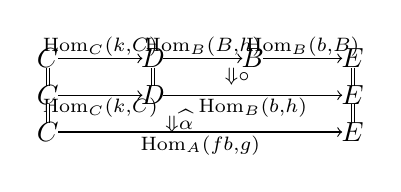
\begin{tikzpicture}[x=0.95em,y=0.95em]
  \node at (-4.6,2.3) {$C$};
  \node at (-0.6,2.3) {$D$};
  \node at (3.2,2.3) {$B$};
  \node at (7.0,2.3) {$E$};
  \draw[->] (-4.2,2.3) -- (-1.0,2.3);
  \node at (-2.6,2.75) {$\scriptstyle\HomC(k,C)$};
  \draw[->] (-0.2,2.3) -- (2.8,2.3);
  \node at (1.3,2.75) {$\scriptstyle\HomB(B,h)$};
  \draw[->] (3.6,2.3) -- (6.6,2.3);
  \node at (5.1,2.75) {$\scriptstyle\HomB(b,B)$};
  \draw[double,double distance=0.6pt] (-4.6,1.95) -- (-4.6,1.25);
  \draw[double,double distance=0.6pt] (-0.6,1.95) -- (-0.6,1.25);
  \draw[double,double distance=0.6pt] (7.0,1.95) -- (7.0,1.25);
  \node at (2.6,1.6) {$\scriptstyle\Downarrow\circ$};
  \node at (-4.6,0.9) {$C$};
  \node at (-0.6,0.9) {$D$};
  \node at (7.0,0.9) {$E$};
  \draw[->] (-4.2,0.9) -- (-1.0,0.9);
  \node at (-2.6,0.42) {$\scriptstyle\HomC(k,C)$};
  \draw[->] (-0.2,0.9) -- (6.6,0.9);
  \node at (3.2,0.42) {$\scriptstyle\HomB(b,h)$};
  \draw[double,double distance=0.6pt] (-4.6,0.55) -- (-4.6,-0.15);
  \draw[double,double distance=0.6pt] (7.0,0.55) -- (7.0,-0.15);
  \node at (0.4,-0.1) {$\scriptstyle\Downarrow\widehat{\alpha}$};
  \node at (-4.6,-0.5) {$C$};
  \node at (7.0,-0.5) {$E$};
  \draw[->] (-4.2,-0.5) -- (6.6,-0.5);
  \node at (1.2,-1.0) {$\scriptstyle\HomA(fb,g)$};
\end{tikzpicture}
\qquad$=$\qquad
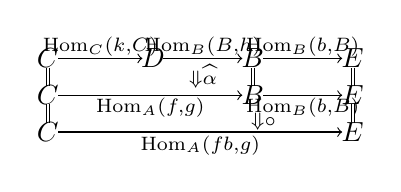
\begin{tikzpicture}[x=0.95em,y=0.95em]
  \node at (-4.6,2.3) {$C$};
  \node at (-0.6,2.3) {$D$};
  \node at (3.2,2.3) {$B$};
  \node at (7.0,2.3) {$E$};
  \draw[->] (-4.2,2.3) -- (-1.0,2.3);
  \node at (-2.6,2.75) {$\scriptstyle\HomC(k,C)$};
  \draw[->] (-0.2,2.3) -- (2.8,2.3);
  \node at (1.3,2.75) {$\scriptstyle\HomB(B,h)$};
  \draw[->] (3.6,2.3) -- (6.6,2.3);
  \node at (5.1,2.75) {$\scriptstyle\HomB(b,B)$};
  \draw[double,double distance=0.6pt] (-4.6,1.95) -- (-4.6,1.25);
  \draw[double,double distance=0.6pt] (3.2,1.95) -- (3.2,1.25);
  \draw[double,double distance=0.6pt] (7.0,1.95) -- (7.0,1.25);
  \node at (1.3,1.6) {$\scriptstyle\Downarrow\widehat{\alpha}$};
  \node at (-4.6,0.9) {$C$};
  \node at (3.2,0.9) {$B$};
  \node at (7.0,0.9) {$E$};
  \draw[->] (-4.2,0.9) -- (2.8,0.9);
  \node at (-0.7,0.42) {$\scriptstyle\HomA(f,g)$};
  \draw[->] (3.6,0.9) -- (6.6,0.9);
  \node at (5.1,0.42) {$\scriptstyle\HomB(b,B)$};
  \draw[double,double distance=0.6pt] (-4.6,0.55) -- (-4.6,-0.15);
  \draw[double,double distance=0.6pt] (7.0,0.55) -- (7.0,-0.15);
  \node at (3.6,-0.1) {$\scriptstyle\Downarrow\circ$};
  \node at (-4.6,-0.5) {$C$};
  \node at (7.0,-0.5) {$E$};
  \draw[->] (-4.2,-0.5) -- (6.6,-0.5);
  \node at (1.2,-1.0) {$\scriptstyle\HomA(fb,g)$};
\end{tikzpicture}
\end{center}
名为 $\circ$ 的两个\trCanonical{}\trCell{}都是复合；由 $\alpha$ 的正合性，$\widehat{\alpha}$ 也是复合，于是由引理 8.3.3 或引理 8.3.8，该粘贴胞腔亦是复合。由 $\beta$ 的正合性，$\widehat{\beta}$ 亦为复合；并再次由引理 8.3.3 或引理 8.3.8 得 $\widehat{\alpha q\cdot f\beta}$ 为复合，这就证明了矩形
$\alpha q\cdot f\beta\colon g(kq)\Rightarrow(fb)p$ 的正合性。
\end{proof}

\subsection*{练习}

\begin{exercise}\label{ex:exact-square-up-to-isomorphism}
对任何\trExactSquare
\begin{center}
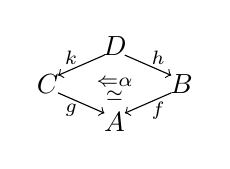
\begin{tikzpicture}[x=1.05em,y=1.05em]
  \node at (0,2.6) {$D$};
  \node at (-2.3,1.3) {$C$};
  \node at (2.3,1.3) {$B$};
  \node at (0,0) {$A$};
  \draw[->] (-0.35,2.3) -- (-1.95,1.6);
  \node at (-1.5,2.2) {$\scriptstyle k$};
  \draw[->] (0.35,2.3) -- (1.95,1.6);
  \node at (1.5,2.2) {$\scriptstyle h$};
  \draw[->] (-1.95,1.0) -- (-0.35,0.3);
  \node at (-1.5,0.4) {$\scriptstyle g$};
  \draw[->] (1.95,1.0) -- (0.35,0.3);
  \node at (1.5,0.4) {$\scriptstyle f$};
  \node at (0,1.35) {$\scriptstyle\Leftarrow\alpha$};
  \node at (0,0.9) {$\scriptstyle\simeq$};
\end{tikzpicture}
\end{center}
证明：将此方块与任何一组\trIsomorphism{} $\beta\colon f'\cong f$、
$\gamma\colon g\cong g'$、$\delta\colon h'\cong h$ 与 $\epsilon\colon k\cong k'$ 复合所得的方块也是正合的。
\end{exercise}

\begin{exercise}\label{ex:prove-trivial-exact-squares}
证明\cref{lem:trivial-exact-squares}。
\end{exercise}
   %
\providecommand{\HomA}{\mathrm{Hom}_{A}}
\providecommand{\HomB}{\mathrm{Hom}_{B}}
\providecommand{\HomC}{\mathrm{Hom}_{C}}
\providecommand{\HomD}{\mathrm{Hom}_{D}}
\providecommand{\HomE}{\mathrm{Hom}_{E}}
\providecommand{\Nearrow}{\rotatebox[origin=c]{45}{$\Rightarrow$}}

\section{逐点右\trKanExtension{}与左\trKanExtension}\label{sec:pointwise-right-and-left-kan-extensions}

在本节中，我们对\trInfinityCategory{}之间的\trFunctor{}给出逐点右%
\trKanExtension{}的四个定义，并证明它们相互等价。我们的证明揭示，右扩张的
一般的 2-范畴式概念（见\cref{def:two-categorical-extension}）就其自身而言
过于微弱。逐点左\trKanExtension{}的对偶理论已由\cref{lem:embedded-extension-lifting}预先展示（见\cref{ex:pointwise-left-extensions}）。

\begin{definition}[扩张对粘贴的稳定性]\label{def:stable-under-pasting}
2-范畴中的一个右扩张图表 $\nu\colon rk\Rightarrow f$ 称为\textbf{与方块
$\alpha$ 粘贴稳定}（stable under pasting with a square），若粘贴复合
\begin{rveq}\label{eq:pasted-composite}
\begin{tikzpicture}[x=0.95em,y=0.95em]
  \node at (0,2.2) {$A$};
  \node at (3.4,2.2) {$C$};
  \node at (0,0) {$B$};
  \draw[->] (0.45,2.2) -- (2.95,2.2);
  \node at (1.7,2.62) {$\scriptstyle f$};
  \draw[->] (0,1.75) -- (0,0.45);
  \node at (-0.42,1.1) {$\scriptstyle k$};
  \draw[->] (0.3,0.25) -- (3.15,2.0);
  \node at (2.15,0.85) {$\scriptstyle r$};
  \node at (1.15,1.4) {$\scriptstyle\Uparrow\nu$};
\end{tikzpicture}
\qquad
\begin{tikzpicture}[x=0.95em,y=0.95em]
  \node at (0,2.3) {$D$};
  \node at (-2.4,1.15) {$A$};
  \node at (2.4,1.15) {$E$};
  \node at (0,0) {$B$};
  \draw[->] (-0.5,1.95) -- (-1.9,1.4);
  \node at (-1.7,1.9) {$\scriptstyle g$};
  \draw[->] (0.5,1.95) -- (1.9,1.4);
  \node at (1.7,1.9) {$\scriptstyle h$};
  \draw[->] (-1.9,0.9) -- (-0.5,0.35);
  \node at (-1.7,0.4) {$\scriptstyle k$};
  \draw[->] (1.9,0.9) -- (0.5,0.35);
  \node at (1.7,0.4) {$\scriptstyle b$};
  \node at (0,1.15) {$\scriptstyle\Leftarrow\alpha$};
\end{tikzpicture}
\qquad
\begin{tikzpicture}[x=0.95em,y=0.95em]
  \node at (0,2.4) {$D$};
  \node at (4.4,2.4) {$A$};
  \node at (8.8,2.4) {$C$};
  \node at (0,0) {$E$};
  \node at (4.4,0) {$B$};
  \draw[->] (0.5,2.4) -- (3.9,2.4);
  \node at (2.2,2.82) {$\scriptstyle g$};
  \draw[->] (4.9,2.4) -- (8.3,2.4);
  \node at (6.6,2.82) {$\scriptstyle f$};
  \draw[->] (0,1.95) -- (0,0.45);
  \node at (-0.47,1.2) {$\scriptstyle h$};
  \draw[->] (4.4,1.95) -- (4.4,0.45);
  \node at (4.87,1.2) {$\scriptstyle k$};
  \draw[->] (0.5,0) -- (3.9,0);
  \node at (2.2,-0.42) {$\scriptstyle b$};
  \draw[->] (4.7,0.3) -- (8.5,2.2);
  \node at (7.0,0.95) {$\scriptstyle r$};
  \node at (2.2,1.2) {$\scriptstyle\Nearrow\alpha$};
  \node at (5.65,1.45) {$\scriptstyle\Uparrow\nu$};
\end{tikzpicture}
\end{rveq}
定义 $fg\colon D\to C$ 沿 $h\colon D\to E$ 的右扩张 $rb\colon E\to C$。
\end{definition}

\begin{theorem}[逐点右扩张]\label{thm:pointwise-right-extensions}
对\trInfinityCosmos{} $\mathcal{K}$ 的\trHomotopyTwoCategory{}中如下图所示的
图表，下列诸条等价：
\begin{center}
\begin{tikzpicture}[x=1.05em,y=1.05em]
  \node at (0,2.2) {$A$};
  \node at (3.4,2.2) {$C$};
  \node at (0,0) {$B$};
  \draw[->] (0.45,2.2) -- (2.95,2.2);
  \node at (1.7,2.62) {$\scriptstyle f$};
  \draw[->] (0,1.75) -- (0,0.45);
  \node at (-0.42,1.1) {$\scriptstyle k$};
  \draw[->] (0.3,0.25) -- (3.15,2.0);
  \node at (2.15,0.85) {$\scriptstyle r$};
  \node at (1.15,1.4) {$\scriptstyle\Uparrow\nu$};
\end{tikzpicture}
\end{center}
\begin{enumerate}[label=(\roman*)]
\item $\nu\colon rk\Rightarrow f$ 在 $\mathfrak{h}\mathcal{K}$ 中定义一个与%
\trExactSquare{}粘贴稳定的右扩张。
\item $\nu\colon rk\Rightarrow f$ 在 $\mathfrak{h}\mathcal{K}$ 中定义一个与%
\trCommaSquare{}粘贴稳定的右扩张。
\item $\nu_{*}\colon \HomB(B,k)\divideontimes\HomC(C,r)\Rightarrow\HomC(C,f)$
在 $\mathbb{M}od(\mathcal{K})$ 中定义一个右扩张。
\item 对任何\trExactSquare
\begin{center}
\begin{tikzpicture}[x=0.95em,y=0.95em]
  \node at (0,2.3) {$D$};
  \node at (-2.4,1.15) {$A$};
  \node at (2.4,1.15) {$E$};
  \node at (0,0) {$B$};
  \draw[->] (-0.5,1.95) -- (-1.9,1.4);
  \node at (-1.7,1.9) {$\scriptstyle g$};
  \draw[->] (0.5,1.95) -- (1.9,1.4);
  \node at (1.7,1.9) {$\scriptstyle h$};
  \draw[->] (-1.9,0.9) -- (-0.5,0.35);
  \node at (-1.7,0.4) {$\scriptstyle k$};
  \draw[->] (1.9,0.9) -- (0.5,0.35);
  \node at (1.7,0.4) {$\scriptstyle b$};
  \node at (0,1.15) {$\scriptstyle\Leftarrow\alpha$};
\end{tikzpicture}
\end{center}
$(\nu g\cdot r\alpha)_{*}\colon \HomE(E,h)\divideontimes\HomC(C,rb)\Rightarrow\HomC(C,fg)$
在 $\mathbb{M}od(\mathcal{K})$ 中定义一个右扩张。
\end{enumerate}
当这些条件成立时，我们称 $r\colon B\to C$ 定义了 $f\colon A\to C$ 沿
$k\colon A\to B$ 的一个\textbf{逐点右扩张}（pointwise right extension）。
\end{theorem}

\begin{proof}
\cref{lem:comma-squares-exact}证明了 (i)$\Rightarrow$(ii)。

为证 (ii)$\Rightarrow$(iii)，设 $\nu\colon rk\Rightarrow f$ 在
$\mathfrak{h}\mathcal{K}$ 中定义一个与\trCommaSquare{}粘贴稳定的右扩张，并考虑
$\mathbb{M}od(\mathcal{K})$ 中的一个\trCell
\begin{center}
\begin{tikzpicture}[x=1.0em,y=1.0em]
  \node at (0,1.2) {$A$};
  \node at (3.6,1.2) {$B$};
  \node at (5.9,1.2) {$\cdots$};
  \node at (9.4,1.2) {$C$};
  \draw[->] (0.5,1.2) -- node[above]{$\scriptstyle\HomB(B,k)$} (3.0,1.2);
  \draw[->] (4.2,1.2) -- node[above]{$\scriptstyle E_{1}$} (5.3,1.2);
  \draw[->] (6.5,1.2) -- node[above]{$\scriptstyle E_{n}$} (7.6,1.2);
  \node at (0,-1.2) {$A$};
  \node at (9.4,-1.2) {$C$};
  \draw[->] (0.5,-1.2) -- node[below]{$\scriptstyle\HomC(C,f)$} (8.9,-1.2);
  \draw[double,double distance=0.6pt] (0,0.7) -- (0,-0.7);
  \draw[double,double distance=0.6pt] (9.4,0.7) -- (9.4,-0.7);
  \node at (4.7,0) {$\scriptstyle\Downarrow\bar{\beta}$};
\end{tikzpicture}
\end{center}
令 $B\overset{q}{\twoheadleftarrow}\vec{E}\overset{p}{\twoheadrightarrow}C$
表示复合双侧纤维化 $E_{1}\divideontimes\cdots\divideontimes E_{n}$。
由注 8.3.12，模映射
\begin{equation*}
\bar{\beta}\colon \HomB(B,k)\divideontimes E_{1}\divideontimes\cdots\divideontimes E_{n}\Rightarrow\HomC(C,f)
\end{equation*}
对应于模映射
\begin{equation*}
\hat{\beta}\colon \HomB(B,k)\divideontimes\HomB(q,B)\divideontimes\HomC(C,p)\Rightarrow\HomC(C,f).
\end{equation*}
由推论 8.4.6 与命题 8.4.7，这类模映射与模映射
\begin{equation*}
\check{\beta}\colon \HomB(q,k)\Rightarrow\HomC(p,f)
\end{equation*}
处于双射之中。由引理 8.1.16，这些模映射与\trHomotopyTwoCategory{}中的如下
2-\trCell{}一一对应
\begin{center}
\begin{tikzpicture}[x=1.05em,y=1.05em]
  \node at (0,2.3) {$\HomB(q,k)$};
  \node at (-3.0,1.15) {$A$};
  \node at (3.0,1.15) {$\vec{E}$};
  \node at (0,0) {$C$};
  \draw[->] (-1.1,2.0) -- (-2.45,1.4);
  \node at (-2.25,1.9) {$\scriptstyle p_{1}$};
  \draw[->] (1.1,2.0) -- (2.45,1.4);
  \node at (2.25,1.9) {$\scriptstyle p_{0}$};
  \draw[->] (-2.55,0.9) -- (-0.5,0.2);
  \node at (-2.05,0.3) {$\scriptstyle f$};
  \draw[->] (2.55,0.9) -- (0.5,0.2);
  \node at (2.05,0.3) {$\scriptstyle p$};
  \node at (0,1.15) {$\scriptstyle\Leftarrow\check{\beta}$};
\end{tikzpicture}
\end{center}

由假设 (ii)，图表
\begin{center}
\begin{tikzpicture}[x=1.0em,y=1.0em]
  \node at (0,2.3) {$\HomB(q,k)$};
  \node at (5.2,2.3) {$A$};
  \node at (9.6,2.3) {$C$};
  \node at (0,0) {$\vec{E}$};
  \node at (5.2,0) {$B$};
  \draw[->] (1.7,2.3) -- (4.4,2.3);
  \node at (3.05,2.72) {$\scriptstyle p_{1}$};
  \draw[->] (6.0,2.3) -- (9.1,2.3);
  \node at (7.4,2.72) {$\scriptstyle f$};
  \draw[->] (0,1.85) -- (0,0.45);
  \node at (-0.52,1.15) {$\scriptstyle p_{0}$};
  \draw[->] (0.5,0) -- (4.4,0);
  \node at (2.5,0.4) {$\scriptstyle q$};
  \draw[->] (5.2,1.85) -- (5.2,0.45);
  \node at (5.67,1.15) {$\scriptstyle k$};
  \draw[->] (5.5,0.3) -- (9.35,2.1);
  \node at (7.9,0.9) {$\scriptstyle r$};
  \node at (2.6,1.15) {$\scriptstyle\Nearrow\phi$};
  \node at (6.3,1.5) {$\scriptstyle\Uparrow\nu$};
\end{tikzpicture}
\end{center}
在 $\mathfrak{h}\mathcal{K}$ 中定义一个右扩张，于是 $\beta$ 经由一个%
\trNaturalTransformation{} $\gamma\colon p\Rightarrow rq$ 唯一地分解过这一
粘贴复合。由命题 8.4.11，这就定义了一个胞腔
$\gamma_{*}\colon \HomC(C,p)\Rightarrow\HomC(C,rq)$，而由推论 8.4.6，它给出
一个\trCanonical{}胞腔
$\hat{\gamma}\colon \HomB(q,B)\divideontimes\HomC(C,p)\Rightarrow\HomC(C,r)$。
再次由注 8.3.12，这就产生了所要的那个唯一分解
\begin{center}
\begin{tikzpicture}[x=1.0em,y=1.0em]
  \node at (0,1.2) {$A$};
  \node at (3.6,1.2) {$B$};
  \node at (5.9,1.2) {$\cdots$};
  \node at (9.4,1.2) {$C$};
  \draw[->] (0.5,1.2) -- node[above]{$\scriptstyle\HomB(B,k)$} (3.0,1.2);
  \draw[->] (4.2,1.2) -- node[above]{$\scriptstyle E_{1}$} (5.3,1.2);
  \draw[->] (6.5,1.2) -- node[above]{$\scriptstyle E_{n}$} (7.6,1.2);
  \node at (0,-1.2) {$A$};
  \node at (9.4,-1.2) {$C$};
  \draw[->] (0.5,-1.2) -- node[below]{$\scriptstyle\HomC(C,f)$} (8.9,-1.2);
  \draw[double,double distance=0.6pt] (0,0.7) -- (0,-0.7);
  \draw[double,double distance=0.6pt] (9.4,0.7) -- (9.4,-0.7);
  \node at (4.7,0) {$\scriptstyle\Downarrow\bar{\beta}$};
\end{tikzpicture}
\quad$=$\quad
\begin{tikzpicture}[x=1.0em,y=1.0em]
  \node at (0,3.4) {$A$};
  \node at (4.6,3.4) {$B$};
  \node at (7.0,3.4) {$\cdots$};
  \node at (11.4,3.4) {$C$};
  \draw[->] (0.5,3.4) -- node[above]{$\scriptstyle\HomB(B,k)$} (4.0,3.4);
  \draw[->] (5.2,3.4) -- node[above]{$\scriptstyle E_{1}$} (6.3,3.4);
  \draw[->] (7.7,3.4) -- node[above]{$\scriptstyle E_{n}$} (8.8,3.4);
  \node at (0,1.7) {$A$};
  \node at (4.6,1.7) {$B$};
  \node at (11.4,1.7) {$C$};
  \draw[->] (0.5,1.7) -- node[above]{$\scriptstyle\HomB(B,k)$} (4.0,1.7);
  \draw[->] (5.2,1.7) -- node[above]{$\scriptstyle\HomC(C,r)$} (10.8,1.7);
  \node at (0,0) {$A$};
  \node at (11.4,0) {$C$};
  \draw[->] (0.5,0) -- node[below]{$\scriptstyle\HomC(C,f)$} (10.8,0);
  \draw[double,double distance=0.6pt] (0,2.9) -- (0,2.2);
  \draw[double,double distance=0.6pt] (0,1.2) -- (0,0.5);
  \draw[double,double distance=0.6pt] (4.6,2.9) -- (4.6,2.2);
  \draw[double,double distance=0.6pt] (11.4,2.9) -- (11.4,2.2);
  \draw[double,double distance=0.6pt] (11.4,1.2) -- (11.4,0.5);
  \node at (7.6,2.55) {$\scriptstyle\exists!\bar{\gamma}$};
  \node at (6.6,0.85) {$\scriptstyle\Downarrow\nu_{*}$};
\end{tikzpicture}
\end{center}

为证 (iii)$\Rightarrow$(iv)，考虑一个使 $\alpha\colon bh\Rightarrow kg$
为正合、且 $\nu_{*}\colon \HomB(B,k)\divideontimes\HomC(C,r)\Rightarrow\HomC(C,f)$
在 $\mathbb{M}od(\mathcal{K})$ 中定义一个右扩张图表的图表
\eqref{eq:pasted-composite}。现在由推论 8.4.6，一个胞腔
\begin{equation*}
\bar{\beta}\colon \HomE(E,h)\divideontimes E_{1}\divideontimes\cdots\divideontimes E_{n}\Rightarrow\HomC(C,fg)
\end{equation*}
对应于一个胞腔
\begin{equation*}
\hat{\beta}\colon \HomA(g,A)\divideontimes\HomE(E,h)\divideontimes E_{1}\divideontimes\cdots\divideontimes E_{n}\Rightarrow\HomC(C,f).
\end{equation*}
由 $\alpha$ 的正合性，这对应于一个胞腔
\begin{equation*}
\hat{\beta}\colon \HomB(b,k)\divideontimes E_{1}\divideontimes\cdots\divideontimes E_{n}\Rightarrow\HomC(C,f),
\end{equation*}
或者等价地，沿复合映射
$\circ\colon \HomB(B,k)\divideontimes\HomB(b,B)\Rightarrow\HomB(b,k)$ 作限制，得到
一个胞腔
\begin{equation*}
\hat{\beta}\colon \HomB(B,k)\divideontimes\HomB(b,B)\divideontimes E_{1}\divideontimes\cdots\divideontimes E_{n}\Rightarrow\HomC(C,f).
\end{equation*}
由于 $B\xrightarrow{\HomC(C,r)}C$ 是 $A\xrightarrow{\HomC(C,f)}C$ 沿
$A\xrightarrow{\HomB(B,k)}B$ 的右扩张，这对应于一个胞腔
\begin{equation*}
\hat{\gamma}\colon \HomB(b,B)\divideontimes E_{1}\divideontimes\cdots\divideontimes E_{n}\Rightarrow\HomC(C,r),
\end{equation*}

它经由推论 8.4.6 转置为一个胞腔
\begin{equation*}
\bar{\gamma}\colon E_{1}\divideontimes\cdots\divideontimes E_{n}\Rightarrow\HomC(C,rb),
\end{equation*}
这就给出了证明模块 $E\xrightarrow{\HomC(C,rb)}C$ 是
$D\xrightarrow{\HomC(C,fg)}C$ 沿 $D\xrightarrow{\HomE(E,h)}E$ 的右扩张所需的
因子分解。要看出这一双射经由与映射
$(\nu g\cdot r\alpha)_{*}\colon \HomE(E,h)\divideontimes\HomC(C,rb)\Rightarrow\HomC(C,fg)$
（即对应于粘贴复合 \eqref{eq:pasted-composite} 的那个映射）的复合来实现，
需要一个稍微精细些的论证；但为此，由\trYonedaLemma，从恒同胞腔
$\mathrm{id}_{\HomC(C,rb)}$ 出发、沿刚才描述的双射逐级向上回溯便已足够。
利用引理 8.1.16，这是直截了当的。

最后，\cref{lem:embedded-extension-lifting}与\cref{lem:trivial-exact-squares}
这一平凡例子共同证明了 (iv)$\Rightarrow$(i)。
\end{proof}

利用\cref{thm:pointwise-right-extensions}的各种刻画，我们可以建立逐点右%
扩张的一些基本稳定性性质。

\begin{corollary}\label{cor:pasting-pointwise-right-extension}
逐点右扩张与一个\trExactSquare{}的粘贴复合 \eqref{eq:pasted-composite} 仍是
一个逐点右扩张。
\end{corollary}

\begin{proof}
由\cref{lem:composites-exact-squares}，两个\trExactSquare{}的粘贴复合仍是%
\trExactSquare，故由\cref{thm:pointwise-right-extensions}(i)，逐点右扩张的
粘贴复合仍保持与正合方块粘贴稳定。
\end{proof}

\begin{corollary}\label{cor:composite-pointwise-extensions}
考虑由\trFunctor{}与\trNaturalTransformation{}构成的如下图所示的图表，其中
$(r,\nu\colon rk\Rightarrow f)$ 是 $f$ 沿 $k$ 的一个逐点右扩张。那么，
$(s,\sigma\colon sh\Rightarrow r)$ 是 $r$ 沿 $h$ 的一个逐点右扩张，当且仅当
$(s,\nu\cdot\sigma k\colon shk\Rightarrow f)$ 是 $f$ 沿 $hk$ 的一个逐点右扩张。
\begin{center}
\begin{tikzpicture}[x=1.05em,y=1.05em]
  \node at (0,3.0) {$A$};
  \node at (3.6,3.0) {$D$};
  \node at (0,1.5) {$B$};
  \node at (0,0) {$C$};
  \draw[->] (0.45,3.0) -- (3.15,3.0);
  \node at (1.8,3.42) {$\scriptstyle f$};
  \draw[->] (0,2.55) -- (0,1.95);
  \node at (-0.42,2.25) {$\scriptstyle k$};
  \draw[->] (0.3,1.75) -- (3.3,2.85);
  \node at (2.05,2.1) {$\scriptstyle r$};
  \node at (1.0,2.55) {$\scriptstyle\Uparrow\nu$};
  \draw[->] (0,1.05) -- (0,0.45);
  \node at (-0.42,0.75) {$\scriptstyle h$};
  \draw[->] (0.35,0.05) to[bend right=25] (3.55,2.75);
  \node at (2.85,0.85) {$\scriptstyle s$};
  \node at (0.8,1.15) {$\scriptstyle\Uparrow\sigma$};
\end{tikzpicture}
\end{center}
\end{corollary}

\begin{proof}
由\cref{thm:pointwise-right-extensions}，\trHomotopyTwoCategory{}中的一个%
\trNaturalTransformation{}是逐点右扩张，当且仅当它到模的\trVirtualEquipment{}中的
共变嵌入是一个右扩张。
在\cref{prop:right-extension-associativity}的双射之下，二元模映射
$\sigma_{*}\colon \HomC(C,h)\divideontimes\HomD(D,s)\Rightarrow\HomD(D,r)$ 与
$(\nu\cdot\sigma k)_{*}\colon \HomC(C,hk)\divideontimes\HomD(D,s)\Rightarrow\HomD(D,f)$\footnote{原书印作
「$\HomC(hk)$」，疑脱首参，应为「$\HomC(C,hk)$」之误，此处径改。——译者注}
相互对应：
\begin{center}
\begin{tikzpicture}[x=1.0em,y=1.0em]
  \node at (0,3.2) {$A$};
  \node at (4.2,3.2) {$B$};
  \node at (8.4,3.2) {$C$};
  \node at (12.6,3.2) {$D$};
  \draw[->] (0.5,3.2) -- node[above]{$\scriptstyle\HomB(B,k)$} (3.7,3.2);
  \draw[->] (4.7,3.2) -- node[above]{$\scriptstyle\HomC(C,h)$} (7.9,3.2);
  \draw[->] (8.9,3.2) -- node[above]{$\scriptstyle\HomD(D,s)$} (12.1,3.2);
  \node at (0,1.6) {$A$};
  \node at (8.4,1.6) {$C$};
  \node at (12.6,1.6) {$D$};
  \draw[->] (0.5,1.6) -- node[below]{$\scriptstyle\HomC(C,hk)$} (7.9,1.6);
  \draw[->] (8.9,1.6) -- node[below]{$\scriptstyle\HomD(D,s)$} (12.1,1.6);
  \node at (0,0) {$A$};
  \node at (12.6,0) {$D$};
  \draw[->] (0.5,0) -- node[below]{$\scriptstyle\HomD(D,f)$} (12.1,0);
  \draw[double,double distance=0.6pt] (0,2.7) -- (0,2.1);
  \draw[double,double distance=0.6pt] (0,1.1) -- (0,0.5);
  \draw[double,double distance=0.6pt] (8.4,2.7) -- (8.4,2.1);
  \draw[double,double distance=0.6pt] (12.6,2.7) -- (12.6,2.1);
  \draw[double,double distance=0.6pt] (12.6,1.1) -- (12.6,0.5);
  \node at (2.1,2.4) {$\scriptstyle\Downarrow\mu$};
  \node at (3.8,0.3) {$\scriptstyle\Downarrow(\nu\cdot\sigma k)_{*}$};
\end{tikzpicture}
\qquad$\mathrel{\leftrightsquigarrow}$\qquad
\begin{tikzpicture}[x=1.0em,y=1.0em]
  \node at (0,3.2) {$A$};
  \node at (4.2,3.2) {$B$};
  \node at (8.4,3.2) {$C$};
  \node at (12.6,3.2) {$D$};
  \draw[->] (0.5,3.2) -- node[above]{$\scriptstyle\HomB(B,k)$} (3.7,3.2);
  \draw[->] (4.7,3.2) -- node[above]{$\scriptstyle\HomC(C,h)$} (7.9,3.2);
  \draw[->] (8.9,3.2) -- node[above]{$\scriptstyle\HomD(D,s)$} (12.1,3.2);
  \node at (0,1.6) {$A$};
  \node at (4.2,1.6) {$B$};
  \node at (12.6,1.6) {$D$};
  \draw[->] (0.5,1.6) -- node[below]{$\scriptstyle\HomB(B,k)$} (3.7,1.6);
  \draw[->] (4.7,1.6) -- node[below]{$\scriptstyle\HomD(D,r)$} (12.1,1.6);
  \node at (0,0) {$A$};
  \node at (12.6,0) {$D$};
  \draw[->] (0.5,0) -- node[below]{$\scriptstyle\HomD(D,f)$} (12.1,0);
  \draw[double,double distance=0.6pt] (0,2.7) -- (0,2.1);
  \draw[double,double distance=0.6pt] (0,1.1) -- (0,0.5);
  \draw[double,double distance=0.6pt] (4.2,2.7) -- (4.2,2.1);
  \draw[double,double distance=0.6pt] (12.6,2.7) -- (12.6,2.1);
  \draw[double,double distance=0.6pt] (12.6,1.1) -- (12.6,0.5);
  \node at (6.6,2.4) {$\scriptstyle\Downarrow\sigma_{*}$};
  \node at (5.8,0.55) {$\scriptstyle\Downarrow\nu_{*}$};
\end{tikzpicture}
\end{center}
于是，由该结果\footnote{原书左图首行第二模印作「$\HomC(C,k)$」，按型算疑为
「$\HomC(C,h)$」之误，此处径改。——译者注}，$\sigma_{*}$ 是一个右扩张当且仅当
$(\nu\cdot\sigma k)_{*}$ 是一个右扩张，即如所断言。
\end{proof}

\subsection*{练习}

\begin{exercise}\label{ex:pointwise-left-extensions}
以\cref{lem:embedded-extension-lifting}为提示，陈述并证明%
\cref{thm:pointwise-right-extensions}的一个对偶版本，以定义%
\trInfinityCosmos{}的\trHomotopyTwoCategory{}中的逐点左扩张。
\end{exercise}

   %
\providecommand{\HomA}{\mathrm{Hom}_{A}}
\providecommand{\HomB}{\mathrm{Hom}_{B}}
\providecommand{\HomC}{\mathrm{Hom}_{C}}
\providecommand{\HomOne}{\mathrm{Hom}_{1}}
\providecommand{\HomJ}{\mathrm{Hom}_{J}}
\providecommand{\colim}{\mathop{\mathrm{colim}}}
\providecommand{\qcTwo}{\mathbf{2}}

\section{虚拟装备中的形式范畴论}\label{sec:formal-category-theory-in-a-virtual-equipment}

我们对模的\trVirtualEquipment{}感兴趣的一个理由是：它把模的演算容纳于
一个\trInfinityCosmos{}之内。一个更有力的辩护则由那些可以在%
\trVirtualEquipment{}内部证明的关于∞-范畴论的定理提供。在本节中，我们
先从模论的观点重新审视\trAdjunction{}与\trFullyFaithful{}函子，然后再把
注意力转向\trInfinityCategory{}之间函子的\trLimit{}与\trColimit。

\begin{proposition}\label{prop:adjunction-counit-characterizations}
对任意一对\trFunctor{} $f\colon B\to A$ 与 $u\colon A\to B$ 以及%
\trNaturalTransformation{} $\epsilon\colon fu\Rightarrow \mathrm{id}_{A}$，
以下诸条等价：
(i) \trNaturalTransformation{} $\epsilon$ 是\trAdjunction{} $f\dashv u$ 的%
\trCounit。

(ii) 表示函子
$\ulcorner\epsilon\cdot f(-)\urcorner\colon \HomB(B,u)\to \HomA(f,A)$ 的
那个一元\trCell{}在模的\trVirtualEquipment{}中定义一个竖直同构：
\begin{center}
\begin{tikzpicture}[x=1em,y=1em]
  \node at (0,1.2)    {$A$};
  \node at (4.6,1.2)  {$B$};
  \node at (0,-1.2)   {$A$};
  \node at (4.6,-1.2) {$B$};
  \draw[->] (0.7,1.2)  -- node[above]{$\scriptstyle\HomB(B,u)$} (3.9,1.2);
  \draw[->] (0.7,-1.2) -- node[below]{$\scriptstyle\HomA(f,A)$} (3.9,-1.2);
  \draw[double] (0,0.7)   -- (0,-0.7);
  \draw[double] (4.6,0.7) -- (4.6,-0.7);
  \node at (2.3,0) {$\scriptstyle\Downarrow$};
\end{tikzpicture}
\end{center}
(iii) 该\trCounit{}定义一个\trExactSquare：
\begin{center}
\begin{tikzpicture}[x=1em,y=1em]
  \node at (0,2.6)    {$A$};
  \node at (-2.3,1.3) {$A$};
  \node at (2.3,1.3)  {$B$};
  \node at (0,0)      {$A$};
  \draw[double,double distance=0.6pt] (-0.35,2.3) -- (-1.95,1.6);
  \draw[->] (0.35,2.3) -- node[above right,pos=0.45]{$\scriptstyle u$} (1.95,1.6);
  \draw[double,double distance=0.6pt] (-1.95,1.0) -- (-0.35,0.3);
  \draw[->] (1.95,1.0) -- node[below right,pos=0.45]{$\scriptstyle f$} (0.35,0.3);
  \node at (0,1.3) {$\scriptstyle\Leftarrow\epsilon$};
\end{tikzpicture}
\end{center}
(iv) 该\trCounit{}定义一个\textbf{绝对的}逐点右扩张图表，它被任何\trFunctor{}
$h\colon A\to C$ 所保持：
\begin{rveq}\label{eq:counit-extension-triangle}
\begin{tikzpicture}[x=1em,y=1em]
  \node at (0,2.2) {$A$};
  \node at (4.6,2.2) {$A$};
  \node at (0,0) {$B$};
  \draw[double,double distance=0.6pt] (0.7,2.2) -- (3.9,2.2);
  \draw[->] (0,1.7) -- node[left]{$\scriptstyle u$} (0,0.5);
  \draw[->] (0.3,0.25) -- node[below,pos=0.55]{$\scriptstyle f$} (4.25,1.95);
  \node at (1.05,1.2) {$\scriptstyle\Uparrow\epsilon$};
\end{tikzpicture}
\end{rveq}
\end{proposition}

\begin{proof}
等价 (i)$\Leftrightarrow$(ii) 经由引理 8.1.17 由命题 4.1.1 得到证明。
说 $\epsilon\colon fu\Rightarrow \mathrm{id}_{A}$ 是正合的，即是说左下方的
二元\trCell{}是一个复合：
\begin{center}
\begin{tikzpicture}[x=1em,y=1em]
  \begin{scope}
    \node at (0,1.2)   {$A$};
    \node at (3.6,1.2) {$A$};
    \node at (8.2,1.2) {$B$};
    \draw[->] (0.65,1.2) -- node[above]{$\scriptstyle\HomA$} (2.95,1.2);
    \draw[->] (4.25,1.2) -- node[above]{$\scriptstyle\HomB(B,u)$} (7.55,1.2);
    \node at (0,-1.2)    {$A$};
    \node at (8.2,-1.2)  {$B$};
    \draw[->] (0.65,-1.2) -- node[below]{$\scriptstyle\HomA(f,A)$} (7.55,-1.2);
    \draw[double] (0,0.7)   -- (0,-0.7);
    \draw[double] (8.2,0.7) -- (8.2,-0.7);
    \node at (4.1,0) {$\scriptstyle\Downarrow\hat{\epsilon}$};
  \end{scope}
  \node at (11.0,0) {$\leftrightsquigarrow$};
  \begin{scope}[shift={(13.4,0)}]
    \node at (0,2.6)   {$A$};
    \node at (2.6,2.6) {$A$};
    \node at (7.2,2.6) {$B$};
    \draw[double,double distance=0.6pt] (0.65,2.6) -- (1.95,2.6);
    \draw[->] (3.25,2.6) -- node[above]{$\scriptstyle\HomB(B,u)$} (6.55,2.6);
    \node at (0,0)   {$A$};
    \node at (2.6,0) {$A$};
    \node at (7.2,0) {$B$};
    \draw[->] (0.65,0) -- node[below]{$\scriptstyle\HomA$} (1.95,0);
    \draw[->] (3.25,0) -- node[below]{$\scriptstyle\HomB(B,u)$} (6.55,0);
    \node at (0,-2.6)  {$A$};
    \node at (7.2,-2.6){$B$};
    \draw[->] (0.65,-2.6) -- node[below]{$\scriptstyle\HomA(f,A)$} (6.55,-2.6);
    \draw[double] (0,2.1)   -- (0,-2.1);
    \draw[double] (7.2,2.1) -- (7.2,-2.1);
    \draw[double] (2.6,2.1) -- (2.6,0.5);
    \node at (1.3,1.3)  {$\scriptstyle\Downarrow\iota$};
    \node at (4.9,-1.3) {$\scriptstyle\Downarrow\hat{\epsilon}$};
  \end{scope}
\end{tikzpicture}
\end{center}
由引理 8.3.3 与引理 8.3.9(i)，这当且仅当右上方的那支一元\trCell{}是一个
复合时成立；而由引理 8.3.9(ii)，这恰好就是 (ii) 所作的断言。于是
(ii)$\Leftrightarrow$(iii)。

为证 (ii)$\Rightarrow$(iv)，我们必须证明左下方所示的这支二元\trCell{}在模的%
\trVirtualEquipment{}中定义一个右扩张图表。
\begin{center}
\begin{tikzpicture}[x=0.95em,y=0.95em]
  \begin{scope}
    \node at (0,1.2)   {$A$};
    \node at (4.4,1.2) {$B$};
    \node at (8.8,1.2) {$C$};
    \draw[->] (0.65,1.2)  -- node[above]{$\scriptstyle\HomB(B,u)$} (3.75,1.2);
    \draw[->] (5.05,1.2)  -- node[above]{$\scriptstyle\HomC(C,hf)$} (8.15,1.2);
    \node at (0,-1.2)  {$A$};
    \node at (8.8,-1.2){$C$};
    \draw[->] (0.65,-1.2) -- node[below]{$\scriptstyle\HomC(C,h)$} (8.15,-1.2);
    \draw[double] (0,0.7)   -- (0,-0.7);
    \draw[double] (8.8,0.7) -- (8.8,-0.7);
    \node at (4.4,0) {$\scriptstyle\Downarrow h\epsilon_{*}$};
  \end{scope}
  \node at (12.0,0) {$\cong$};
  \begin{scope}[shift={(14.4,0)}]
    \node at (0,1.2)   {$A$};
    \node at (4.4,1.2) {$B$};
    \node at (8.8,1.2) {$C$};
    \draw[->] (0.65,1.2)  -- node[above]{$\scriptstyle\HomA(f,A)$} (3.75,1.2);
    \draw[->] (5.05,1.2)  -- node[above]{$\scriptstyle\HomC(C,hf)$} (8.15,1.2);
    \node at (0,-1.2)  {$A$};
    \node at (8.8,-1.2){$C$};
    \draw[->] (0.65,-1.2) -- node[below]{$\scriptstyle\HomC(C,h)$} (8.15,-1.2);
    \draw[double] (0,0.7)   -- (0,-0.7);
    \draw[double] (8.8,0.7) -- (8.8,-0.7);
    \node at (4.4,0) {$\scriptstyle\Downarrow$};
  \end{scope}
  \node at (25.6,0) {$=$};
  \begin{scope}[shift={(27.6,0)}]
    \node at (0,2.6)   {$A$};
    \node at (4.4,2.6) {$B$};
    \node at (9.2,2.6) {$C$};
    \draw[->] (0.65,2.6)  -- node[above]{$\scriptstyle\HomA(f,A)$} (3.75,2.6);
    \draw[->] (5.05,2.6)  -- node[above]{$\scriptstyle\HomC(C,hf)$} (8.55,2.6);
    \node at (0,0)    {$A$};
    \node at (3.2,0)  {$A$};
    \node at (9.2,0)  {$C$};
    \draw[->] (0.65,0) -- node[below]{$\scriptstyle\HomA$} (2.55,0);
    \draw[->] (3.85,0) -- node[below]{$\scriptstyle\HomC(C,h)$} (8.55,0);
    \node at (0,-2.6)  {$A$};
    \node at (9.2,-2.6){$C$};
    \draw[->] (0.65,-2.6) -- node[below]{$\scriptstyle\HomC(C,h)$} (8.55,-2.6);
    \draw[double] (0,2.1)   -- (0,-2.1);
    \draw[double] (9.2,2.1) -- (9.2,-2.1);
    \draw[->] (4.4,2.1) -- node[right]{$\scriptstyle f$} (4.4,0.5);
    \node at (1.6,1.3)  {$\scriptstyle\Downarrow\rho$};
    \node at (6.9,1.3)  {$\scriptstyle\Downarrow\rho$};
    \node at (6.2,-1.3) {$\scriptstyle\Downarrow\circ$};
  \end{scope}
\end{tikzpicture}
\end{center}
由 (ii)，这个二元\trCell{}同构于中图所示形状的一个二元\trCell。\footnote{原书
中、右二图首行第二模均印作「$\HomA(A,hf)$」，按型算疑为「$\HomC(C,hf)$」
之误，此处径改。——译者注}
事实上，
引理 8.1.16 与注 8.3.13 可以用来验证：右图公式所定义的\trCell{}与竖直
同构 $\ulcorner\epsilon\cdot f(-)\urcorner\colon \HomB(B,u)\simeq \HomA(f,A)$
相复合，便产生左图的那个二元\trCell。这正是我们在\cref{lem:hom-binary-cell}
中对二元\trCell{}采用记号「$\epsilon$」的原因。于是，由%
\cref{lem:canonical-restriction-cells}，这些二元\trCell{}是模的%
\trVirtualEquipment{}中的右扩张，故可见 (ii)$\Rightarrow$(iv)。

(iv)$\Rightarrow$(i) 的证明可以完全在\trHomotopyTwoCategory{}中进行，而且不需要
「逐点的」这一形容词。事实上，这是引理 2.3.7 中留作练习 2.3.iii 的那
一部分之 op-对偶。
\end{proof}

由此可知，沿\trRightAdjoint{}的右扩张与沿\trLeftAdjoint{}的左扩张都易于
计算：

\begin{corollary}\label{cor:extensions-along-adjoints}
任何\trFunctor{}沿\trRightAdjoint{} $u\colon A\to B$ 的逐点右扩张，由其沿%
\trLeftAdjoint{} $f\colon B\to A$ 的限制给出；而任何\trFunctor{}沿一个%
\trLeftAdjoint{}的逐点左扩张，由其沿该\trRightAdjoint{}的限制给出：
\begin{center}
\begin{tikzpicture}[x=1em,y=1em]
  \begin{scope}
    \node at (0,2.2) {$A$};
    \node at (4.6,2.2) {$C$};
    \draw[->] (0.7,2.2) -- node[above]{$\scriptstyle h$} (3.9,2.2);
    \draw[->] (0,1.7) -- node[left]{$\scriptstyle u$} (0,0.5);
    \draw[->,dashed] (0.3,0.25) -- node[below,pos=0.6]{$\scriptstyle\mathrm{ran}_{u}h\cong hf$} (4.25,1.95);
    \node at (1.05,1.2) {$\scriptstyle\Uparrow h\epsilon$};
    \node at (0,0) {$B$};
  \end{scope}
  \begin{scope}[shift={(8.0,0)}]
    \node at (0,2.2) {$B$};
    \node at (4.6,2.2) {$C$};
    \draw[->] (0.7,2.2) -- node[above]{$\scriptstyle g$} (3.9,2.2);
    \draw[->] (0,1.7) -- node[left]{$\scriptstyle f$} (0,0.5);
    \draw[->,dashed] (0.3,0.25) -- node[below,pos=0.6]{$\scriptstyle\mathrm{lan}_{f}g\cong gu$} (4.25,1.95);
    \node at (1.05,1.2) {$\scriptstyle\Downarrow g\eta$};
    \node at (0,0) {$A$};
  \end{scope}
\end{tikzpicture}
\end{center}
\end{corollary}

\begin{proof}
在\cref{prop:adjunction-counit-characterizations}中说\trAdjunction{}
$f\dashv u$ 的\trCounit{} $\epsilon$ 是一个绝对的逐点右扩张，意即：对任何%
\trFunctor{} $h\colon A\to C$，图
\begin{center}
\begin{tikzpicture}[x=1em,y=1em]
  \node at (0,2.2) {$A$};
  \node at (3.0,2.2) {$A$};
  \node at (7.6,2.2) {$C$};
  \draw[double,double distance=0.6pt] (0.7,2.2) -- (2.3,2.2);
  \draw[->] (3.7,2.2) -- node[above]{$\scriptstyle h$} (6.9,2.2);
  \draw[->] (0,1.7) -- node[left]{$\scriptstyle u$} (0,0.5);
  \draw[->,dashed] (0.3,0.25) -- node[below,pos=0.55]{$\scriptstyle f$} (7.25,1.95);
  \node at (1.0,1.2) {$\scriptstyle\Uparrow\epsilon$};
  \node at (0,0) {$B$};
\end{tikzpicture}
\end{center}
是一个逐点右扩张。特别地，$hf\simeq\mathrm{ran}_{u}h$。
\end{proof}

第 3 章中的推论 3.5.6 描述了\trInfinityCategory{}之间\trFullyFaithful{}%
函子的若干等价刻画，其中一种刻画隐含地是模论的：\trFunctor{}
$k\colon A\to B$ 是\trFullyFaithful，当且仅当
$\ulcorner\mathrm{id}_{k}\urcorner\colon \qcTwo\sim \HomB(k,k)$ 是
$A\times A$ 之上的一个\trFiberedEquivalence。在模的\trVirtualEquipment{}%
中，这一条件可以用若干种方式重新表述：

\begin{lemma}\label{lem:fully-faithful-characterizations}
\trFunctor{} $k\colon A\to B$ 是\trFullyFaithful，当下列诸等价条件中的
任何一条成立时：
(i) 该方块是正合的：
\begin{center}
\begin{tikzpicture}[x=1em,y=1em]
  \node at (0,2.6)    {$A$};
  \node at (-2.3,1.3) {$A$};
  \node at (2.3,1.3)  {$A$};
  \node at (0,0)      {$B$};
  \draw[double,double distance=0.6pt] (-0.35,2.3) -- (-1.95,1.6);
  \draw[double,double distance=0.6pt] (0.35,2.3)  -- (1.95,1.6);
  \draw[->] (-1.95,1.0) -- node[below left,pos=0.45]{$\scriptstyle k$} (-0.35,0.3);
  \draw[->] (1.95,1.0)  -- node[below right,pos=0.45]{$\scriptstyle k$} (0.35,0.3);
\end{tikzpicture}
\end{center}
(ii) 模映射 $\ulcorner\mathrm{id}_{k}\urcorner$ 在模的\trVirtualEquipment{}%
中定义一个竖直同构：
\begin{center}
\begin{tikzpicture}[x=1em,y=1em]
  \node at (0,1.2)    {$A$};
  \node at (4.6,1.2)  {$A$};
  \node at (0,-1.2)   {$A$};
  \node at (4.6,-1.2) {$A$};
  \draw[->] (0.7,1.2)  -- node[above]{$\scriptstyle\HomA$} (3.9,1.2);
  \draw[->] (0.7,-1.2) -- node[below]{$\scriptstyle\HomB(k,k)$} (3.9,-1.2);
  \draw[double] (0,0.7)   -- (0,-0.7);
  \draw[double] (4.6,0.7) -- (4.6,-0.7);
  \node at (2.3,0) {$\scriptstyle\Downarrow$};
\end{tikzpicture}
\end{center}
\end{lemma}

\begin{proof}
在拆开诸定义之后，这一等价性由引理 8.3.9 的零元复合与一元复合、以及
引理 8.3.10 的复合关系 $\HomA\otimes\HomA\simeq\HomA$ 得出。
\end{proof}

众所周知，沿\trFullyFaithful{}函子的逐点左扩张与逐点右扩张是真正的
扩张，其意义在于：那个泛\trNaturalTransformation{}是一个同构。

\begin{proposition}[沿全忠实函子的扩张]\label{prop:extensions-along-fully-faithful}
若 $k\colon A\to B$ 是\trFullyFaithful，则对任何逐点右扩张，
\trNaturalTransformation{} $\nu\colon rk\Rightarrow f$ 是一个同构。
\begin{center}
\begin{tikzpicture}[x=1em,y=1em]
  \node at (0,2.2) {$A$};
  \node at (4.6,2.2) {$C$};
  \draw[->] (0.7,2.2) -- node[above]{$\scriptstyle f$} (3.9,2.2);
  \draw[->] (0,1.7) -- node[left]{$\scriptstyle k$} (0,0.5);
  \draw[->,dashed] (0.3,0.25) -- node[below,pos=0.6]{$\scriptstyle r$} (4.25,1.95);
  \node at (1.05,1.2) {$\scriptstyle\Uparrow\nu$};
  \node at (0,0) {$B$};
\end{tikzpicture}
\end{center}
\end{proposition}

\begin{proof}
把陈述中的逐点右扩张与\cref{lem:fully-faithful-characterizations}的%
\trExactSquare{}粘贴起来，便产生一个逐点右扩张图表；它在\trHomotopyTwoCategory{}%
中的\trUniversalProperty{}可以用来构造 $\nu$ 的一个逆同构，并证明它定义
一个双侧逆：
\begin{center}
\begin{tikzpicture}[x=1em,y=1em]
  \begin{scope}
    \node at (0,1.9)   {$A$};
    \node at (3.4,1.9) {$C$};
    \node at (0,0)     {$A$};
    \draw[->] (0.7,1.9) -- node[above]{$\scriptstyle f$} (2.7,1.9);
    \draw[double] (0,1.4) -- (0,0.5);
    \draw[->,dashed] (0.3,0.2) -- node[below,pos=0.55]{$\scriptstyle rk$} (3.05,1.7);
    \node at (0.85,1.15) {$\scriptstyle\Uparrow\nu$};
  \end{scope}
  \begin{scope}[shift={(7.2,0)}]
    \node at (0,1.9)   {$A$};
    \node at (3.4,1.9) {$C$};
    \node at (0,0)     {$A$};
    \draw[->] (0.7,1.9) -- node[above]{$\scriptstyle f$} (2.7,1.9);
    \draw[double] (0,1.4) -- (0,0.5);
    \draw[->,dashed] (0.3,0.2) -- node[below,pos=0.55]{$\scriptstyle f$} (3.05,1.7);
    \node at (0.9,1.15) {$\scriptstyle\Uparrow\mathrm{id}_{f}$};
  \end{scope}
  \node at (13.4,0.95) {$=$};
  \begin{scope}[shift={(15.6,0)}]
    \node at (0,1.9)   {$A$};
    \node at (3.4,1.9) {$C$};
    \node at (0,0)     {$A$};
    \draw[->] (0.7,1.9) -- node[above]{$\scriptstyle f$} (2.7,1.9);
    \draw[double] (0,1.4) -- (0,0.5);
    \draw[->,dashed] (0.35,0.35) -- node[above left,pos=0.5]{$\scriptstyle rk$} (2.9,1.65);
    \draw[->] (0.3,0.1) to[bend right=30] node[below,pos=0.6]{$\scriptstyle f$} (3.1,1.75);
    \node at (0.85,1.3)  {$\scriptstyle\Uparrow\nu$};
    \node at (2.15,0.6)  {$\scriptstyle\Uparrow\exists!$};
  \end{scope}
\end{tikzpicture}
\end{center}
\end{proof}

\begin{proposition}\label{prop:right-adjoint-fully-faithful}
一个\trRightAdjoint{} $u\colon A\to B$ 是\trFullyFaithful，当且仅当%
\trCounit{} $\epsilon\colon fu\Rightarrow \mathrm{id}_{A}$ 是一个同构。
\end{proposition}

\begin{proof}
若 $f\dashv u$ 带有\trCounit{} $\epsilon\colon fu\Rightarrow \mathrm{id}_{A}$，
则由\cref{prop:adjunction-counit-characterizations}，\trCounit{}
$\epsilon\colon fu\Rightarrow \mathrm{id}_{A}$ 是正合的。若 $u$ 是%
\trFullyFaithful，则由\cref{lem:composites-exact-squares}，下方的复合
矩形也是正合的。
\begin{center}
\begin{tikzpicture}[x=1em,y=1em]
  \node at (2.2,3.4)  {$A$};
  \node at (0.9,2.3)  {$A$};
  \node at (3.5,2.3)  {$A$};
  \node at (-0.6,1.2) {$A$};
  \node at (2.2,1.2)  {$B$};
  \node at (0.9,0.1)  {$A$};
  \draw[double,double distance=0.6pt] (1.75,3.15) -- (1.35,2.6);
  \draw[double,double distance=0.6pt] (2.65,3.15) -- (3.05,2.6);
  \draw[double,double distance=0.6pt] (0.55,2.0)  -- (0.0,1.5);
  \draw[double,double distance=0.6pt] (0.25,0.4)  -- (0.7,0.95);
  \draw[->] (1.35,2.1)  -- node[below left,pos=0.4]{$\scriptstyle u$} (1.85,1.55);
  \draw[->] (3.05,2.1)  -- node[below right,pos=0.4]{$\scriptstyle u$} (2.6,1.55);
  \draw[->] (1.95,1.0)  -- node[below right,pos=0.5]{$\scriptstyle f$} (1.35,0.3);
  \node at (0.85,1.2) {$\scriptstyle\Leftarrow\epsilon$};
\end{tikzpicture}
\end{center}
拆开\cref{def:exact-square}，这就是说（由引理 8.3.10 与引理 8.3.9）：
$\epsilon$ 在定义 8.4.12 的反变嵌入之下的像诱导了模的一个等价
$\epsilon^{*}\colon \HomA\simeq \HomA(fu,A)$。由命题 8.4.11，这个嵌入是%
\trFullyFaithful，从而可知 $\epsilon\colon fu\Rightarrow \mathrm{id}_{A}$
是一个同构。
反之，设 $f\dashv u$ 带有可逆的\trCounit{}%
$\epsilon\colon fu\cong\mathrm{id}_{A}$。练习 3.6.ii 与推论 4.1.3 的诸\trFiberedEquivalence
\begin{equation*}
\HomA\xrightarrow[\simeq]{\ \epsilon^{*}\ }\HomA(fu,A)
\xrightarrow[\simeq]{\ \ulcorner u(-)\cdot\eta\urcorner\ }\HomB(u,u)
\end{equation*}
复合起来，便定义了模映射 $\ulcorner\mathrm{id}_{u}\urcorner\colon \HomA\Rightarrow \HomB(u,u)$。于是，由\cref{lem:fully-faithful-characterizations}，
$u$ 是\trFullyFaithful。
\end{proof}

现在我们转向由\trInfinityCategory{}标引的图表的\trLimit{}与\trColimit。
回忆定义 1.2.23：一个\trInfinityCosmos{} $\mathcal{K}$ 是%
\trCartesianClosed，如果对任何 $J\in\mathcal{K}$ 都存在一个%
\trCosmologicalFunctor{} $(-)^{J}\colon \mathcal{K}\to\mathcal{K}$，装备有
一个\trSimplicial{}自然同构
\begin{equation*}
\mathrm{Fun}(X\times J,A)\cong \mathrm{Fun}(X,A^{J}).
\end{equation*}
由此，$A$ 中 $J$ 形图表之\trInfinityCategory{}里的\trElement{}
$f\colon 1\to A^{J}$ 双射地对应于\trInfinityCategory{}之间的\trFunctor{}
$f\colon J\to A$。在这样的上下文中，定义 2.3.8 把一个由\trInfinityCategory{}%
标引的图表 $f\colon J\to A$ 的\trLimit{}与\trColimit{}分别定义为绝对右
提升与绝对左提升：
\begin{center}
\begin{tikzpicture}[x=1em,y=1em]
  \begin{scope}
    \node at (2.8,2.2) {$A$};
    \draw[->] (2.8,1.7) -- node[right]{$\scriptstyle\Delta$} (2.8,0.5);
    \draw[->,dashed] (0.35,0.25) -- node[above left,pos=0.5]{$\scriptstyle\lim f$} (2.45,1.95);
    \node at (1.5,1.0) {$\scriptstyle\Downarrow\epsilon$};
    \node at (0,0)   {$1$};
    \node at (5.6,0) {$A^{J}$};
    \draw[->] (0.7,0) -- node[below]{$\scriptstyle f$} (4.9,0);
  \end{scope}
  \begin{scope}[shift={(9.6,0)}]
    \node at (2.8,2.2) {$A$};
    \draw[->] (2.8,1.7) -- node[right]{$\scriptstyle\Delta$} (2.8,0.5);
    \draw[->,dashed] (0.35,0.25) -- node[above left,pos=0.5]{$\scriptstyle\colim f$} (2.45,1.95);
    \node at (1.4,1.0) {$\scriptstyle\Uparrow\eta$};
    \node at (0,0)   {$1$};
    \node at (5.6,0) {$A^{J}$};
    \draw[->] (0.7,0) -- node[below]{$\scriptstyle f$} (4.9,0);
  \end{scope}
\end{tikzpicture}
\end{center}

现在我们论证：这样的\trLimit{}与\trColimit{}也可以表述为逐点%
\trKanExtension，从而把先前展开的理论拓广到那些未必\trCartesianClosed{}%
\trInfinityCosmos。

\begin{definition}\label{def:limit-colimit-diagrams}
由\trInfinityCategory{}构成的图表 $f\colon J\to A$ 的一个\textbf{\trLimit}，
由如下左图所示的一个逐点右扩张给出；而由\trInfinityCategory{}构成的图表
$f\colon J\to A$ 的一个\textbf{\trColimit}，由如下右图所示的一个逐点左
扩张给出。
\begin{center}
\begin{tikzpicture}[x=1em,y=1em]
  \begin{scope}
    \node at (0,2.2) {$J$};
    \node at (4.6,2.2) {$A$};
    \draw[->] (0.7,2.2) -- node[above]{$\scriptstyle f$} (3.9,2.2);
    \draw[->] (0,1.7) -- node[left]{$\scriptstyle !$} (0,0.5);
    \draw[->,dashed] (0.3,0.25) -- node[below right,pos=0.55]{$\scriptstyle\lim f$} (4.25,1.95);
    \node at (1.05,1.2) {$\scriptstyle\Uparrow\epsilon$};
    \node at (0,0) {$1$};
  \end{scope}
  \begin{scope}[shift={(8.4,0)}]
    \node at (0,2.2) {$J$};
    \node at (4.6,2.2) {$A$};
    \draw[->] (0.7,2.2) -- node[above]{$\scriptstyle f$} (3.9,2.2);
    \draw[->] (0,1.7) -- node[left]{$\scriptstyle !$} (0,0.5);
    \draw[->,dashed] (0.3,0.25) -- node[below right,pos=0.55]{$\scriptstyle\colim f$} (4.25,1.95);
    \node at (1.05,1.2) {$\scriptstyle\Downarrow\eta$};
    \node at (0,0) {$1$};
  \end{scope}
\end{tikzpicture}
\end{center}
如同定义 2.3.8 中那样，我们把\trNaturalTransformation{} $\epsilon$ 与
$\eta$ 分别称为\textbf{极限\trCone}与\textbf{余极限\trCone}。我们的第一
个任务是调和这些定义：
\end{definition}

\begin{proposition}\label{prop:limit-pointwise-extension-transpose}
在一个\trCartesianClosed{}\trInfinityCosmos{}中，任何由如下右图所示绝对
右提升图表所编码的\trLimit{}都转置而定义如下左图所示的一个逐点右扩张图表：
\begin{center}
\begin{tikzpicture}[x=1em,y=1em]
  \begin{scope}
    \node at (0,2.2) {$J$};
    \node at (4.6,2.2) {$A$};
    \draw[->] (0.7,2.2) -- node[above]{$\scriptstyle f$} (3.9,2.2);
    \draw[->] (0,1.7) -- node[left]{$\scriptstyle !$} (0,0.5);
    \draw[->,dashed] (0.3,0.25) -- node[below right,pos=0.55]{$\scriptstyle\lim f$} (4.25,1.95);
    \node at (1.05,1.2) {$\scriptstyle\Uparrow\epsilon$};
    \node at (0,0) {$1$};
  \end{scope}
  \node at (8.0,1.1) {$\leftrightsquigarrow$};
  \begin{scope}[shift={(10.6,0)}]
    \node at (2.8,2.2) {$A$};
    \draw[->] (2.8,1.7) -- node[right]{$\scriptstyle\Delta$} (2.8,0.5);
    \draw[->,dashed] (0.35,0.25) -- node[above left,pos=0.5]{$\scriptstyle\lim f$} (2.45,1.95);
    \node at (1.5,1.0) {$\scriptstyle\Downarrow\epsilon$};
    \node at (0,0)   {$1$};
    \node at (5.6,0) {$A^{J}$};
    \draw[->] (0.7,0) -- node[below]{$\scriptstyle f$} (4.9,0);
  \end{scope}
\end{tikzpicture}
\end{center}
反之，任何这种形状的逐点右扩张图表都转置而定义 $A$ 中的一个\trLimit。
\end{proposition}

\begin{proof}
由\cref{lem:limit-transpose}，如下左图所示的绝对右提升图表的%
\trUniversalProperty{}转置为这样一个右扩张图表的\trUniversalProperty——
它对与\trPullback{}方块作粘贴保持稳定：
\begin{center}
\begin{tikzpicture}[x=1em,y=1em]
  \begin{scope}
    \node at (2.8,2.2) {$A$};
    \draw[->] (2.8,1.7) -- node[right]{$\scriptstyle\Delta$} (2.8,0.5);
    \draw[->,dashed] (0.35,0.25) -- node[above left,pos=0.5]{$\scriptstyle\lim f$} (2.45,1.95);
    \node at (1.5,1.0) {$\scriptstyle\Downarrow\epsilon$};
    \node at (0,0)   {$1$};
    \node at (5.6,0) {$A^{J}$};
    \draw[->] (0.7,0) -- node[below]{$\scriptstyle f$} (4.9,0);
  \end{scope}
  \node at (8.4,1.1) {$\leftrightsquigarrow$};
  \begin{scope}[shift={(11.0,0)}]
    \node at (0,2.2) {$J$};
    \node at (4.6,2.2) {$A$};
    \draw[->] (0.7,2.2) -- node[above]{$\scriptstyle f$} (3.9,2.2);
    \draw[->] (0,1.7) -- node[left]{$\scriptstyle !$} (0,0.5);
    \draw[->,dashed] (0.3,0.25) -- node[below right,pos=0.55]{$\scriptstyle\lim f$} (4.25,1.95);
    \node at (1.05,1.2) {$\scriptstyle\Uparrow\epsilon$};
    \node at (0,0) {$1$};
  \end{scope}
  \begin{scope}[shift={(19.4,0)}]
    \node at (0,2.2)   {$X\times J$};
    \node at (5.0,2.2) {$J$};
    \node at (9.6,2.2) {$A$};
    \draw[->] (1.5,2.2) -- node[above]{$\scriptstyle\pi$} (4.3,2.2);
    \draw[->] (5.7,2.2) -- node[above]{$\scriptstyle f$} (8.9,2.2);
    \node at (0,0) {$X$};
    \node at (5.0,0) {$1$};
    \draw[->] (0,1.7) -- node[left]{$\scriptstyle\pi$} (0,0.5);
    \draw[->] (0.7,0) -- node[below]{$\scriptstyle !$} (4.3,0);
    \draw[->] (5.0,1.7) -- node[right]{$\scriptstyle !$} (5.0,0.5);
    \node at (0.9,1.5) {$\scriptstyle\lrcorner$};
    \draw[->,dashed] (5.3,0.25) -- node[below right,pos=0.55]{$\scriptstyle\lim f$} (9.25,1.95);
    \node at (6.1,1.2) {$\scriptstyle\Uparrow\epsilon$};
  \end{scope}
\end{tikzpicture}
\end{center}
由于余定义域为终\trInfinityCategory{}的余跨度上的\trCommaSquare{}归约为%
\trPullback，我们从定理 9.3.3(ii) 得知：$\epsilon\colon \Delta\lim f\Rightarrow f$
是一个绝对右提升图表，当且仅当 $\epsilon\colon \lim f\,!\Rightarrow f$ 是一个逐点右扩张。
\end{proof}

在经典\trCategory{}理论中，有一个众所周知的公式把逐点右%
\trKanExtension{}的值「逐点地」计算为\trLimit。一个对偶的余极限公式
计算逐点左 \trKanExtension。这些公式如今便可以回收过来——本质上是作为
重言式。

\begin{proposition}\label{prop:limits-from-slices}
对任何如下左图所示的逐点右扩张与任何\trElement{} $b\colon 1\to B$，
\trElement{} $rb\colon 1\to C$ 是如下右图所示图表的\trLimit：
\begin{center}
\begin{tikzpicture}[x=1em,y=1em]
  \begin{scope}
    \node at (0,2.2) {$A$};
    \node at (4.6,2.2) {$C$};
    \draw[->] (0.7,2.2) -- node[above]{$\scriptstyle f$} (3.9,2.2);
    \draw[->] (0,1.7) -- node[left]{$\scriptstyle k$} (0,0.5);
    \draw[->,dashed] (0.3,0.25) -- node[below,pos=0.6]{$\scriptstyle r$} (4.25,1.95);
    \node at (1.05,1.2) {$\scriptstyle\Uparrow\nu$};
    \node at (0,0) {$B$};
  \end{scope}
  \begin{scope}[shift={(8.8,1.1)}]
    \node at (0,0) {$\HomB(b,k)$};
    \node at (5.6,0) {$A$};
    \node at (10.2,0) {$C$};
    \draw[double,->] (1.7,0) -- node[above]{$\scriptstyle p_{1}$} (4.9,0);
    \draw[->] (6.3,0) -- node[above]{$\scriptstyle f$} (9.5,0);
  \end{scope}
\end{tikzpicture}
\end{center}
而对任何如下左图所示的逐点左扩张与任何\trElement{} $b\colon 1\to B$，
\trElement{} $\ell b\colon 1\to C$ 是如下右图所示图表的\trColimit：
\begin{center}
\begin{tikzpicture}[x=1em,y=1em]
  \begin{scope}
    \node at (0,2.2) {$A$};
    \node at (4.6,2.2) {$C$};
    \draw[->] (0.7,2.2) -- node[above]{$\scriptstyle f$} (3.9,2.2);
    \draw[->] (0,1.7) -- node[left]{$\scriptstyle k$} (0,0.5);
    \draw[->,dashed] (0.3,0.25) -- node[below,pos=0.6]{$\scriptstyle\ell$} (4.25,1.95);
    \node at (1.05,1.2) {$\scriptstyle\Downarrow\lambda$};
    \node at (0,0) {$B$};
  \end{scope}
  \begin{scope}[shift={(8.8,1.1)}]
    \node at (0,0) {$\HomB(k,b)$};
    \node at (5.6,0) {$A$};
    \node at (10.2,0) {$C$};
    \draw[->] (1.7,0) -- node[above]{$\scriptstyle p_{0}$} (4.9,0);
    \draw[->] (6.3,0) -- node[above]{$\scriptstyle f$} (9.5,0);
  \end{scope}
\end{tikzpicture}
\end{center}
\end{proposition}

\begin{proof}
由定理 9.3.3(ii)，复合
\begin{center}
\begin{tikzpicture}[x=1em,y=1em]
  \node at (0,2.2)   {$\HomB(b,k)$};
  \node at (6.0,2.2) {$A$};
  \node at (10.6,2.2){$C$};
  \draw[double,->] (2.3,2.2) -- node[above]{$\scriptstyle p_{1}$} (5.3,2.2);
  \draw[->] (6.7,2.2) -- node[above]{$\scriptstyle f$} (9.9,2.2);
  \node at (0,0) {$1$};
  \node at (6.0,0) {$B$};
  \draw[->] (0,1.7) -- node[left]{$\scriptstyle !$} (0,0.5);
  \draw[->] (0.7,0) -- node[below]{$\scriptstyle b$} (5.3,0);
  \draw[->] (6.0,1.7) -- node[left]{$\scriptstyle k$} (6.0,0.5);
  \draw[->,dashed] (6.3,0.25) -- node[below,pos=0.55]{$\scriptstyle r$} (10.25,1.95);
  \node at (3.0,1.1) {$\scriptstyle\Nearrow\phi$};
  \node at (7.1,1.2) {$\scriptstyle\Uparrow\nu$};
\end{tikzpicture}
\end{center}
是一个逐点右扩张。由\cref{def:limit-colimit-diagrams}，这可以解释为：
$rb\colon 1\to C$ 定义了图表 $f\colon A\to C$ 沿
$p_{1}\colon \HomB(b,k)\twoheadrightarrow A$ 的限制的\trLimit。\footnote{原书印作
「$rb\colon 1\to B$」，按命题陈述与本证明（$rb\colon 1\to C$ 为所论
极限之\trElement）疑为「$1\to C$」之误，此处径改。——译者注}
\end{proof}

在定义 2.2.1 中，$A$ 中的\trInitial{}元素与\trTerminal{}元素分别定义为
唯一\trFunctor{} $!\colon A\to 1$ 的\trLeftAdjoint{}或\trRightAdjoint
\begin{center}
\begin{tikzpicture}[x=1em,y=1em]
  \node at (0,0)   {$1$};
  \node at (4.6,0) {$A$};
  \draw[->] (0.7,0.55) to[bend left=25] node[above]{$\scriptstyle i$} (3.9,0.55);
  \node at (2.3,0.27) {$\scriptstyle\dashv$};
  \draw[->] (3.9,0) -- node[below]{$\scriptstyle !$} (0.7,0);
  \node at (2.3,-0.3) {$\scriptstyle\dashv$};
  \draw[->] (0.7,-0.55) to[bend right=25] node[below]{$\scriptstyle t$} (3.9,-0.55);
\end{tikzpicture}
\end{center}
或者等价地（由例 2.3.10），定义为 $A^{\varnothing}\simeq 1$ 中%
\trEmptyDiagram{}的\trColimit{}或\trLimit。如例 2.3.11 中所观察到的，
一个\trInitial{}元素也可以刻画为恒同图表 $\mathrm{id}_{A}\colon A\to A$
的一个\emph{\trLimit}，而一个\trTerminal{}元素也可以刻画为其\emph{\trColimit}；我们
现在就未必\trCartesianClosed{}\trInfinityCosmos{}来证明这一点：

\begin{proposition}\label{prop:terminal-initial-elements-via-id}
对一个\trInfinityCategory{} $A$：
(i) 一个\trElement{} $t\colon 1\to A$ 是\trTerminal{}的，当且仅当它为恒同
函子 $\mathrm{id}_{A}\colon A\to A$ 定义一个\trColimit；此时，\trAdjunction{}
$!\dashv t$ 的\trUnit{}定义该余极限\trCone。
(ii) 一个\trElement{} $i\colon 1\to A$ 是\trInitial{}的，当且仅当它为恒同
函子 $\mathrm{id}_{A}\colon A\to A$ 定义一个\trLimit；此时，\trAdjunction{}
$i\dashv !$ 的\trCounit{}定义该极限\trCone。
\end{proposition}

\begin{proof}
我们证明 (ii)。由定义 2.2.1，一个\trElement{} $i\colon 1\to A$ 是%
\trInitial{}的，当且仅当它为唯一\trFunctor{} $!\colon A\to 1$ 定义一个%
\trRightAdjoint。若这一\trAdjunction{}存在，则由%
\cref{prop:adjunction-counit-characterizations}，该\trCounit{}定义一个
逐点右扩张图表
\begin{center}
\begin{tikzpicture}[x=1em,y=1em]
  \node at (0,2.2) {$A$};
  \node at (4.6,2.2) {$A$};
  \draw[double,double distance=0.6pt] (0.7,2.2) -- (3.9,2.2);
  \draw[->] (0,1.7) -- node[left]{$\scriptstyle !$} (0,0.5);
  \draw[->,dashed] (0.3,0.25) -- node[below,pos=0.55]{$\scriptstyle i$} (4.25,1.95);
  \node at (1.05,1.2) {$\scriptstyle\Uparrow\epsilon$};
  \node at (0,0) {$1$};
\end{tikzpicture}
\end{center}
而由\cref{def:limit-colimit-diagrams}，这就把 $i$ 表达为图表
$\mathrm{id}_{A}\colon A\to A$ 的一个\trLimit。

反之，我们必须证明：一个逐点右扩张图表 $(i,\ \epsilon\colon i!\Rightarrow\mathrm{id}_{A})$
会给出一个带\trCounit{} $\epsilon$ 的\trAdjunction{}
$i\dashv !$。由引理 2.2.2，只需证明 $\epsilon i=\mathrm{id}_{i}$。由
须化的自然性（见引理 B.1.3），$\epsilon$ 与其自身的水平复合给出等式
$i!\epsilon\cdot\epsilon=\epsilon\cdot\epsilon i!$。由于\trInfinityCategory{}
$1$ 是 2-终的，$i!\epsilon=\mathrm{id}_{i!}$，于是这归约为如下粘贴等式：
\begin{center}
\begin{tikzpicture}[x=1em,y=1em]
  \begin{scope}
    \node at (0,1.9) {$A$};
    \node at (2.8,1.9) {$A$};
    \draw[double,double distance=0.6pt] (0.7,1.9) -- (2.1,1.9);
    \draw[->] (0,1.4) -- node[left]{$\scriptstyle !$} (0,0.5);
    \draw[->,dashed] (0.3,0.25) -- node[below,pos=0.55]{$\scriptstyle i$} (2.45,1.7);
    \node at (0.95,1.15) {$\scriptstyle\Uparrow\epsilon$};
    \node at (0,0) {$1$};
  \end{scope}
  \node at (5.2,0.95) {$=$};
  \begin{scope}[shift={(7.2,0)}]
    \node at (0,1.9) {$A$};
    \node at (2.8,1.9) {$A$};
    \draw[double,double distance=0.6pt] (0.7,1.9) -- (2.1,1.9);
    \draw[->] (0,1.4) -- node[left]{$\scriptstyle !$} (0,0.5);
    \draw[->] (0.3,0.35) -- node[above left,pos=0.5]{$\scriptstyle i$} (2.5,1.7);
    \draw[->] (0.25,0.05) to[bend right=30] node[below,pos=0.6]{$\scriptstyle i$} (2.6,1.8);
    \node at (0.9,1.25) {$\scriptstyle\Uparrow\epsilon$};
    \node at (1.95,0.6) {$\scriptstyle\Uparrow\epsilon i$};
    \node at (0,0) {$1$};
  \end{scope}
\end{tikzpicture}
\end{center}
由右扩张\trUniversalProperty{}中的唯一性陈述，即得
$\epsilon i=\mathrm{id}_{i}$，如所需。
\end{proof}

回忆定义 2.4.5：一个\trFunctor{} $k\colon I\to J$ 是\textbf{末的}
（final），如果对任何\trInfinityCategory{} $A$，方块
\begin{center}
\begin{tikzpicture}[x=1em,y=1em]
  \node at (0,2.2)    {$A$};
  \node at (5.2,2.2)  {$A$};
  \node at (0,-1.2)   {$A^{J}$};
  \node at (5.2,-1.2) {$A^{I}$};
  \draw[double,double distance=0.6pt] (0.7,2.2) -- (4.5,2.2);
  \draw[->] (0,1.7) -- node[left]{$\scriptstyle\Delta$} (0,-0.5);
  \draw[->] (5.2,1.7) -- node[right]{$\scriptstyle\Delta$} (5.2,-0.5);
  \draw[->] (0.7,-1.2) -- node[below]{$\scriptstyle A^{k}$} (4.5,-1.2);
\end{tikzpicture}
\end{center}
保持并反映一切绝对左提升图表。对偶地，一个\trFunctor{} $k\colon I\to J$
是\textbf{始的}（initial），如果该方块保持并反映一切绝对右提升图表。现在
我们可以给这些概念一个更简洁的表述。

\begin{definition}\label{def:final-initial-exact-squares}
一个\trFunctor{} $k\colon I\to J$ 是\textbf{末函子}，当且仅当如下左图的
方块是正合的；是\textbf{始函子}，当且仅当如下右图的方块是正合的。
\begin{center}
\begin{tikzpicture}[x=1em,y=1em]
  \begin{scope}
    \node at (0,2.6)    {$I$};
    \node at (-2.3,1.3) {$1$};
    \node at (2.3,1.3)  {$J$};
    \node at (0,0)      {$1$};
    \draw[->] (-0.35,2.3) -- node[above left,pos=0.45]{$\scriptstyle !$} (-1.95,1.6);
    \draw[->] (0.35,2.3)  -- node[above right,pos=0.45]{$\scriptstyle k$} (1.95,1.6);
    \draw[double,double distance=0.6pt] (-1.95,1.0) -- (-0.35,0.3);
    \draw[->] (1.95,1.0)  -- node[above right,pos=0.5]{$\scriptstyle !$} (0.35,0.3);
  \end{scope}
  \begin{scope}[shift={(8.4,0)}]
    \node at (0,2.6)    {$I$};
    \node at (-2.3,1.3) {$J$};
    \node at (2.3,1.3)  {$1$};
    \node at (0,0)      {$1$};
    \draw[->] (-0.35,2.3) -- node[above left,pos=0.45]{$\scriptstyle k$} (-1.95,1.6);
    \draw[->] (0.35,2.3)  -- node[above right,pos=0.45]{$\scriptstyle !$} (1.95,1.6);
    \draw[double,double distance=0.6pt] (1.95,1.0) -- (0.35,0.3);
    \draw[->] (-1.95,1.0) -- node[above left,pos=0.5]{$\scriptstyle !$} (-0.35,0.3);
  \end{scope}
\end{tikzpicture}
\end{center}
注意到\trFunctor{} $!\colon J\to 1$ 在右侧与在左侧分别由模
$J\xrightarrow{J}1$ 与 $1\xrightarrow{J}J$ 所表示。于是我们看到：
$k\colon I\to J$ 是末函子，当且仅当如下左图的跨度映射是模的%
\trVirtualEquipment{}中的一个复合
\begin{center}
\begin{tikzpicture}[x=1em,y=1em]
  \begin{scope}
    \node at (0,2.6)    {$\HomJ(J,k)$};
    \node at (-3.4,1.3) {$1$};
    \node at (3.4,1.3)  {$J$};
    \node at (0,0)      {$J$};
    \draw[->] (-1.5,2.3) -- node[above left,pos=0.45]{$\scriptstyle !$} (-2.9,1.6);
    \draw[->] (1.5,2.3)  -- node[above right,pos=0.45]{$\scriptstyle p_{0}$} (2.9,1.6);
    \draw[->] (0,2.1) -- node[right]{$\scriptstyle p_{0}$} (0,0.5);
    \draw[->] (-0.3,-0.2) -- node[below left,pos=0.45]{$\scriptstyle !$} (-2.9,1.0);
    \draw[double,double distance=0.6pt] (0.3,-0.2) -- (2.9,1.0);
  \end{scope}
  \begin{scope}[shift={(10.4,0)}]
    \node at (0,2.6)    {$\HomJ(k,J)$};
    \node at (-3.4,1.3) {$J$};
    \node at (3.4,1.3)  {$1$};
    \node at (0,0)      {$J$};
    \draw[->] (-1.5,2.3) -- node[above left,pos=0.45]{$\scriptstyle p_{1}$} (-2.9,1.6);
    \draw[->] (1.5,2.3)  -- node[above right,pos=0.45]{$\scriptstyle !$} (2.9,1.6);
    \draw[->] (0,2.1) -- node[right]{$\scriptstyle p_{1}$} (0,0.5);
    \draw[double,double distance=0.6pt] (-0.3,-0.2) -- (-2.9,1.0);
    \draw[->] (0.3,-0.2) -- node[below right,pos=0.45]{$\scriptstyle !$} (2.9,1.0);
  \end{scope}
\end{tikzpicture}
\end{center}
而 $k\colon I\to J$ 是始函子，当且仅当如上右图的跨度映射是一个复合。
\end{definition}

\begin{remark}\label{rem:strongly-exact-finality}
如\cref{dig:strong-exactness}中所论，在 $(\infty,1)$-范畴的%
\trInfinityCosmos{}中，\trExactSquare{}自动是强正合的；此时，末函子所
满足的\trUniversalProperty{}便可以被富集。由于从 $1$ 到 $J$ 的模归约为
$J$ 上的\trDiscreteCartesianFibration，在这类上下文中，$k\colon I\to J$ 的
末性蕴涵：对每一个\trDiscreteCartesianFibration{}
$p\colon E\twoheadrightarrow J$，映射
\begin{rveq}\label{eq:final-characterization}
\begin{tikzpicture}[x=1em,y=1em]
  \node at (0,0)    {$\mathrm{Fun}_{J}(J,E)$};
  \node at (8.2,0)  {$\mathrm{Fun}_{J}(\HomJ(J,k),E)$};
  \node at (17.4,0) {$\mathrm{Fun}_{J}(I,E)$};
  \draw[->] (2.9,0)  -- node[above]{$\scriptstyle-\circ p_{0}$} node[below]{$\scriptstyle\simeq$} (5.4,0);
  \draw[->] (11.2,0) -- node[above]{$\scriptstyle-\circ\ulcorner\mathrm{id}_{k}\urcorner$} node[below]{$\scriptstyle\simeq$} (14.4,0);
  \draw[->] (16.4,-0.55) to[bend left=15] node[below]{$\scriptstyle-\circ k$} node[above]{$\scriptstyle\simeq$} (1.0,-0.55);
\end{tikzpicture}
\end{rveq}
是一个 Kan 复形的等价——第一个等价由强正合性给出，第二个等价由推论
5.7.19 的\trYonedaLemma{}给出。在拟范畴的\trInfinityCosmos{}中，条件
\eqref{eq:final-characterization} 刻画了拟范畴之间的末函子，Lurie 将这
一定义归于 Joyal [78, 4.1.1.1]。
\end{remark}

正如刚才所论证的，在 $(\infty,1)$-范畴的\trInfinityCosmos{}中，我们的
末函子概念蕴涵这一刻画；现在我们再论证逆方向也成立。推论 12.3.8 证明：
$(\infty,1)$-范畴的诸\trInfinityCosmos{}是强封闭的，意即：模的右扩张与
右\trLifting{}总是存在，并且满足一个表述为 Kan 复形之等价的%
\trUniversalProperty{}，而不只是在\trVirtualEquipment{}中诸\trCell{}的
一个双射。于是，由\cref{ex:closed-virtual-equipment}的强类比，
\eqref{eq:final-characterization}
对 $J$ 上的一切\trDiscreteCartesianFibration{}都定义一个等价，当且仅当%
\cref{def:final-initial-exact-squares}的方块是强正合的。因此，在拟范畴的%
\trInfinityCosmos{}中，我们的末函子概念等价于标准定义。

现在我们证明：\trLimit{}在沿始函子换指标时被保持并反映。

\begin{proposition}\label{prop:limits-along-initial-functors}
若 $k\colon I\to J$ 是始函子且 $f\colon J\to A$ 是任何图表，则 $f$ 的一个%
\trLimit{}也定义 $fk\colon I\to A$ 的一个\trLimit；反之，若 $fk\colon I\to A$
的\trLimit{}存在，则它也定义 $f\colon J\to A$ 的一个\trLimit。
\end{proposition}

\begin{proof}
由\cref{def:limit-colimit-diagrams}，$f$ 的一个\trLimit{}定义如下左图的
一个逐点右扩张；由推论 9.3.4 与\cref{def:final-initial-exact-squares}，
它又给出如下右图的另一个逐点右扩张。
\begin{center}
\begin{tikzpicture}[x=1em,y=1em]
  \begin{scope}
    \node at (0,2.2) {$J$};
    \node at (4.6,2.2) {$A$};
    \draw[->] (0.7,2.2) -- node[above]{$\scriptstyle f$} (3.9,2.2);
    \draw[->] (0,1.7) -- node[left]{$\scriptstyle !$} (0,0.5);
    \draw[->,dashed] (0.3,0.25) -- node[below,pos=0.6]{$\scriptstyle\ell$} (4.25,1.95);
    \node at (1.05,1.2) {$\scriptstyle\Uparrow\nu$};
    \node at (0,0) {$1$};
  \end{scope}
  \begin{scope}[shift={(9.0,0)}]
    \node at (0,2.2) {$I$};
    \node at (3.2,2.2) {$J$};
    \node at (7.8,2.2) {$A$};
    \draw[->] (0.7,2.2) -- node[above]{$\scriptstyle k$} (2.5,2.2);
    \draw[->] (3.9,2.2) -- node[above]{$\scriptstyle f$} (7.1,2.2);
    \draw[->] (0,1.7) -- node[left]{$\scriptstyle !$} (0,0.5);
    \draw[->] (3.2,1.7) -- node[right]{$\scriptstyle !$} (3.2,0.5);
    \node at (0,0)    {$1$};
    \node at (3.2,0)  {$1$};
    \draw[double,double distance=0.6pt] (0.7,0) -- (2.5,0);
    \draw[->,dashed] (3.5,0.25) -- node[below,pos=0.55]{$\scriptstyle\ell$} (7.45,1.95);
    \node at (4.3,1.2) {$\scriptstyle\Uparrow\nu$};
  \end{scope}
\end{tikzpicture}
\end{center}
由\cref{def:limit-colimit-diagrams}，这告诉我们 $\ell$ 是 $fk$ 的一个%
\trLimit。

反之，设给定一个逐点右扩张图表
\begin{center}
\begin{tikzpicture}[x=1em,y=1em]
  \node at (0,2.2) {$I$};
  \node at (4.6,2.2) {$A$};
  \draw[->] (0.7,2.2) -- node[above]{$\scriptstyle fk$} (3.9,2.2);
  \draw[->] (0,1.7) -- node[left]{$\scriptstyle !$} (0,0.5);
  \draw[->,dashed] (0.3,0.25) -- node[below,pos=0.6]{$\scriptstyle\ell$} (4.25,1.95);
  \node at (1.05,1.2) {$\scriptstyle\Uparrow\mu$};
  \node at (0,0) {$1$};
\end{tikzpicture}
\end{center}
由定理 9.3.3(iii)，这意味着：对从 $1$ 到 $A$ 的模的任何相容序列
$E_{1}\divideontimes\cdots\divideontimes E_{n}$，与
$\mu\colon \HomOne(1,!)\divideontimes \HomA(A,\ell)\Rightarrow \HomA(A,fk)$\footnote{原书
此模印作「$\mathrm{Hom}_{!}(1,!)$」，下标疑为「$1$」之误，此处径改。——译者注}
作复合，便在诸\trCell{}
$E_{1}\divideontimes\cdots\divideontimes E_{n}\Rightarrow \HomA(A,\ell)$
与如下左图的诸\trCell{}之间定义了一个双射：
\begin{center}
\begin{tikzpicture}[x=0.95em,y=0.95em]
  \begin{scope}
    \node at (0,1.2)   {$I$};
    \node at (3.2,1.2) {$1$};
    \node at (8.2,1.2) {$A$};
    \draw[->] (0.65,1.2)  -- node[above]{$\scriptstyle\HomOne(1,!)$} (2.55,1.2);
    \draw[->,dotted] (3.9,1.2)  -- node[above]{$\scriptstyle\vec{E}$} (7.55,1.2);
    \node at (0,-1.2)  {$I$};
    \node at (8.2,-1.2){$A$};
    \draw[->] (0.65,-1.2) -- node[below]{$\scriptstyle\HomA(A,fk)$} (7.55,-1.2);
    \draw[double] (0,0.7)   -- (0,-0.7);
    \draw[double] (8.2,0.7) -- (8.2,-0.7);
    \node at (4.1,0) {$\scriptstyle\Downarrow$};
  \end{scope}
  \node at (11.2,0) {$\leftrightsquigarrow$};
  \begin{scope}[shift={(13.6,0)}]
    \node at (0,1.2)    {$J$};
    \node at (3.6,1.2)  {$I$};
    \node at (6.8,1.2)  {$1$};
    \node at (11.8,1.2) {$A$};
    \draw[->] (0.65,1.2)  -- node[above]{$\scriptstyle\HomJ(k,J)$} (2.95,1.2);
    \draw[->] (4.25,1.2)  -- node[above]{$\scriptstyle\HomOne(1,!)$} (6.15,1.2);
    \draw[->,dotted] (7.5,1.2)  -- node[above]{$\scriptstyle\vec{E}$} (11.15,1.2);
    \node at (0,-1.2)   {$J$};
    \node at (11.8,-1.2){$A$};
    \draw[->] (0.65,-1.2) -- node[below]{$\scriptstyle\HomA(A,f)$} (11.15,-1.2);
    \draw[double] (0,0.7)    -- (0,-0.7);
    \draw[double] (11.8,0.7) -- (11.8,-0.7);
    \node at (5.9,0) {$\scriptstyle\Downarrow$};
  \end{scope}
\end{tikzpicture}
\end{center}
由推论 8.4.6，左图的诸\trCell{}与右图的诸\trCell{}处于双射之中。

说 $k\colon I\to J$ 是始函子，据\cref{def:final-initial-exact-squares}，
意即：由恒同所诱导的、从 $J$ 到 $1$ 的模的映射
$\HomJ(k,J)\divideontimes \HomOne(1,!)\Rightarrow \HomOne(1,!)$ 是一个复合。
于是，右图的诸\trCell{}与如下形状的诸\trCell{}处于双射之中：
\begin{center}
\begin{tikzpicture}[x=1em,y=1em]
  \node at (0,1.2)   {$J$};
  \node at (3.4,1.2) {$1$};
  \node at (8.4,1.2) {$A$};
  \draw[->] (0.65,1.2)  -- node[above]{$\scriptstyle\HomOne(1,!)$} (2.75,1.2);
  \draw[->,dotted] (4.1,1.2)  -- node[above]{$\scriptstyle\vec{E}$} (7.75,1.2);
  \node at (0,-1.2)  {$J$};
  \node at (8.4,-1.2){$A$};
  \draw[->] (0.65,-1.2) -- node[below]{$\scriptstyle\HomA(A,f)$} (7.75,-1.2);
  \draw[double] (0,0.7)   -- (0,-0.7);
  \draw[double] (8.4,0.7) -- (8.4,-0.7);
  \node at (4.2,0) {$\scriptstyle\Downarrow$};
\end{tikzpicture}
\end{center}

这一复合双射断言：对应于模恒同胞腔 $\mathrm{id}\colon \HomA(A,\ell)\Rightarrow\HomA(A,\ell)$ 的\trCell{}
$\nu\colon \HomOne(1,!)\divideontimes \HomA(A,\ell)\Rightarrow \HomA(A,f)$，
把 $1\xrightarrow{\HomA(A,\ell)}A$ 显示为 $J\xrightarrow{\HomA(A,f)}A$
沿 $J\xrightarrow{\HomOne(1,!)}1$ 的右扩张。拆开定义 $\nu$ 的那些双射，
我们看到 $\nu k=\mu$。于是 $\nu\colon \ell!\Rightarrow f$ 是一个逐点右
扩张，而由\cref{prop:limit-pointwise-extension-transpose}我们得出结论：
$\ell\colon 1\to A$ 定义 $f\colon J\to A$ 的一个\trLimit，如所需。
\end{proof}

尚待完成的是把定理 2.4.2——右伴随保持\trLimit{}而左伴随保持%
\trColimit——拓广到由一般\trInfinityCosmos{}中的\trInfinityCategory{}%
标引的图表。在定理 9.5.7 中，我们将证明这一结果的一个推广，它覆盖由一支
模加权的\trLimit{}与\trColimit，其意义我们即将引入。

\subsection*{练习}

\begin{exercise}\label{ex:unit-exact-square}
证明：\trAdjunction{} $f\dashv u$ 的\trUnit{}定义一个\trExactSquare：
\begin{center}
\begin{tikzpicture}[x=1em,y=1em]
  \node at (0,2.6)    {$B$};
  \node at (-2.3,1.3) {$A$};
  \node at (2.3,1.3)  {$B$};
  \node at (0,0)      {$B$};
  \draw[->] (-0.35,2.3) -- node[above left,pos=0.45]{$\scriptstyle f$} (-1.95,1.6);
  \draw[double,double distance=0.6pt] (0.35,2.3) -- (1.95,1.6);
  \draw[->] (-1.95,1.0) -- node[below left,pos=0.45]{$\scriptstyle u$} (-0.35,0.3);
  \draw[double,double distance=0.6pt] (1.95,1.0) -- (0.35,0.3);
  \node at (0,1.3) {$\scriptstyle\Leftarrow\eta$};
\end{tikzpicture}
\end{center}
\end{exercise}

\begin{exercise}\label{ex:mate-exact-square}
证明：任何如下左图所示、涉及平行伴随 $f\dashv u$ 与 $k\dashv r$ 的方块
$\alpha$，只要其对应（mate）定义一个同构，便是正合的。
\begin{center}
\begin{tikzpicture}[x=1em,y=1em]
  \begin{scope}
    \node at (0,2.6)    {$D$};
    \node at (-2.3,1.3) {$C$};
    \node at (2.3,1.3)  {$B$};
    \node at (0,0)      {$A$};
    \draw[->] (-0.35,2.3) -- node[above left,pos=0.45]{$\scriptstyle k$} (-1.95,1.6);
    \draw[->] (0.35,2.3)  -- node[above right,pos=0.45]{$\scriptstyle h$} (1.95,1.6);
    \draw[->] (-1.95,1.0) -- node[below left,pos=0.45]{$\scriptstyle g$} (-0.35,0.3);
    \draw[->] (1.95,1.0)  -- node[below right,pos=0.45]{$\scriptstyle f$} (0.35,0.3);
    \node at (0,1.3) {$\scriptstyle\Leftarrow\alpha$};
  \end{scope}
  \node at (5.6,1.3) {$\leftrightsquigarrow$};
  \begin{scope}[shift={(9.2,0)}]
    \node at (0,2.6)    {$D$};
    \node at (-2.3,1.3) {$C$};
    \node at (2.3,1.3)  {$B$};
    \node at (0,0)      {$A$};
    \draw[->] (-1.95,1.6) -- node[above left,pos=0.45]{$\scriptstyle r$} (-0.35,2.3);
    \draw[->] (0.35,2.3)  -- node[above right,pos=0.45]{$\scriptstyle h$} (1.95,1.6);
    \draw[->] (-1.95,1.0) -- node[below left,pos=0.45]{$\scriptstyle g$} (-0.35,0.3);
    \draw[->] (-0.35,-0.3) -- node[below right,pos=0.45]{$\scriptstyle u$} (1.95,1.0);
    \node at (0,1.3)  {$\scriptstyle\cong\Downarrow\beta$};
  \end{scope}
\end{tikzpicture}
\end{center}
\end{exercise}

\begin{exercise}\label{ex:right-adjoint-final-square}
证明：若 $k\colon I\to J$ 是一个\trRightAdjoint，则方块
\begin{center}
\begin{tikzpicture}[x=1em,y=1em]
  \node at (0,2.6)    {$I$};
  \node at (-2.3,1.3) {$1$};
  \node at (2.3,1.3)  {$J$};
  \node at (0,0)      {$1$};
  \draw[->] (-0.35,2.3) -- node[above left,pos=0.45]{$\scriptstyle !$} (-1.95,1.6);
  \draw[->] (0.35,2.3)  -- node[above right,pos=0.45]{$\scriptstyle k$} (1.95,1.6);
  \draw[double,double distance=0.6pt] (-1.95,1.0) -- (-0.35,0.3);
  \draw[->] (1.95,1.0)  -- node[above right,pos=0.5]{$\scriptstyle !$} (0.35,0.3);
\end{tikzpicture}
\end{center}
是正合的，从而重新证明命题 2.4.6。
\end{exercise}

   %
\providecommand{\HomA}{\mathrm{Hom}_{A}}
\providecommand{\HomB}{\mathrm{Hom}_{B}}
\providecommand{\HomC}{\mathrm{Hom}_{C}}
\providecommand{\colim}{\mathop{\mathrm{colim}}\nolimits}
\providecommand{\ran}{\mathop{\mathrm{ran}}\nolimits}
\providecommand{\lan}{\mathop{\mathrm{lan}}\nolimits}

\section{∞-范畴中的\trWeightedLimit{}与\trWeightedColimit{}}\label{sec:weighted-limits-and-colimits-in-infinity-categories}

在本节中，我们把由定义 9.4.7 所编码的诸\trInfinityCategory{}之间图表的\trLimit{}与%
\trColimit{}推广为由一支\trModule{}加权的\trLimit{}与\trColimit%
。\trWeightedLimit{}与\trWeightedColimit{}的概念涵盖了定义 9.4.7（见%
\cref{ex:ordinary-limits-as-weighted}），而且从模的\trVirtualEquipment{}的观点来看
是相当自然的。
这可以理解为 A.6 节中在\trEnrichedCategory{}的语境下所引入理论的∞-范畴式版本，不过
从一开始，我们就允许诸\textbf{权}（weight）取为\textbf{\trProfunctor}（profunctor），如练习
A.6.iv 中那样。

\begin{definition}\label{def:weighted-limits-colimits}
给定一支\trModule{} $A\xrightarrow{W}B$ 与一个\trFunctor{} $f\colon A\to C$，一个函子
$\lim_{W}f\colon B\to C$ 定义 $f$ 的\textbf{$W$-\trWeightedLimit}，若它共变地表示
$\HomC(C,f)$ 沿 $W$ 的右\trExtension{}。对偶地，给定 $A\xrightarrow{W}B$ 与一个%
\trFunctor{} $g\colon B\to C$，一个函子 $\colim_{W}g\colon A\to C$ 定义 $g$ 的%
\textbf{$W$-\trWeightedColimit}，若它反变地表示 $\HomC(g,C)$ 穿过 $W$ 的右\trLifting{}。
\begin{center}
\begin{tikzpicture}[x=1.0em,y=1.0em]
  \begin{scope}
    \node at (0,1.4)   {$A$};
    \node at (3.4,1.4) {$B$};
    \node at (8.6,1.4) {$C$};
    \draw[->] (0.55,1.4) -- node[above]{$\scriptstyle W$} (2.75,1.4);
    \draw[->,dashed] (3.95,1.4) -- node[above]{$\scriptstyle\HomC(C,\lim_{W}f)$} (7.95,1.4);
    \draw[double,double distance=0.6pt] (0,1.05) -- (0,-1.05);
    \draw[double,double distance=0.6pt] (8.6,1.05) -- (8.6,-1.05);
    \node at (4.3,0) {$\scriptstyle\Downarrow\lambda$};
    \node at (0,-1.4)   {$A$};
    \node at (8.6,-1.4) {$C$};
    \draw[->] (0.55,-1.4) -- node[below]{$\scriptstyle\HomC(C,f)$} (7.95,-1.4);
  \end{scope}
  \qquad
  \begin{scope}[shift={(12.2,0)}]
    \node at (0,1.4)   {$C$};
    \node at (5.2,1.4) {$A$};
    \node at (8.6,1.4) {$B$};
    \draw[->,dashed] (0.55,1.4) -- node[above]{$\scriptstyle\HomC(\colim_{W}g,C)$} (4.55,1.4);
    \draw[->] (5.75,1.4) -- node[above]{$\scriptstyle W$} (7.95,1.4);
    \draw[double,double distance=0.6pt] (0,1.05) -- (0,-1.05);
    \draw[double,double distance=0.6pt] (8.6,1.05) -- (8.6,-1.05);
    \node at (4.3,0) {$\scriptstyle\Downarrow\gamma$};
    \node at (0,-1.4)   {$C$};
    \node at (8.6,-1.4) {$B$};
    \draw[->] (0.55,-1.4) -- node[below]{$\scriptstyle\HomC(g,C)$} (7.95,-1.4);
  \end{scope}
\end{tikzpicture}
\end{center}
\end{definition}

将\cref{def:weighted-limits-colimits}与定理 9.3.3(iii) 相比较，我们看到：诸逐点右%
\trExtension{}与逐点左\trExtension{}可以理解为\trWeightedLimit{}与\trWeightedColimit{}的特例
（另见例 A.6.15）。

\begin{lemma}\label{lem:pointwise-extensions-weighted}
\trFunctor{} $f\colon A\to C$ 沿 $k\colon A\to B$ 的逐点右\trExtension{}，是 $f$ 由
$A\xrightarrow{\HomB(B,k)}B$ 加权的\trLimit{}；而 $f$ 沿 $k$ 的逐点左\trExtension{}，是
$f$ 由 $B\xrightarrow{\HomB(k,B)}A$ 加权的\trColimit{}。
\begin{center}
\begin{tikzpicture}[x=1.05em,y=1.05em]
  \begin{scope}
    \node at (0,1.6)   {$A$};
    \node at (4.6,1.6) {$C$};
    \node at (0,0)     {$B$};
    \draw[->] (0.55,1.6) -- node[above]{$\scriptstyle f$} (4.0,1.6);
    \draw[->] (0,1.1)   -- node[left]{$\scriptstyle k$} (0,0.5);
    \draw[->,dashed] (0.3,0.25) -- node[below,pos=0.6]{$\scriptstyle\ran_{k}f\cong\lim_{\HomB(B,k)}f$} (4.3,1.35);
    \node at (0.85,1.05) {$\scriptstyle\Uparrow\nu$};
  \end{scope}
  \qquad
  \begin{scope}[shift={(14.5,0)}]
    \node at (0,1.6)   {$A$};
    \node at (4.6,1.6) {$C$};
    \node at (0,0)     {$B$};
    \draw[->] (0.55,1.6) -- node[above]{$\scriptstyle f$} (4.0,1.6);
    \draw[->] (0,1.1)   -- node[left]{$\scriptstyle k$} (0,0.5);
    \draw[->,dashed] (0.3,0.25) -- node[below,pos=0.6]{$\scriptstyle\lan_{k}f\cong\colim_{\HomB(k,B)}f$} (4.3,1.35);
    \node at (0.85,1.05) {$\scriptstyle\Downarrow\lambda$};
  \end{scope}
\end{tikzpicture}
\end{center}
\end{lemma}

\begin{proof}
由定理 9.3.3(iii)，一个逐点右\trExtension{}定义诸模的一个右\trExtension{}，而一个逐点
左\trExtension{}定义诸模的一个右\trLifting{}：
\begin{center}
\begin{tikzpicture}[x=1.0em,y=1.0em]
  \begin{scope}
    \node at (0,1.4)   {$A$};
    \node at (4.2,1.4) {$B$};
    \node at (9.4,1.4) {$C$};
    \draw[->] (0.55,1.4) -- node[above]{$\scriptstyle\HomB(B,k)$} (3.55,1.4);
    \draw[->,dashed] (4.75,1.4) -- node[above]{$\scriptstyle\HomC(C,\ran_{k}f)$} (8.75,1.4);
    \draw[double,double distance=0.6pt] (0,1.05) -- (0,-1.05);
    \draw[double,double distance=0.6pt] (9.4,1.05) -- (9.4,-1.05);
    \node at (4.7,0) {$\scriptstyle\Downarrow\nu_{*}$};
    \node at (0,-1.4)   {$A$};
    \node at (9.4,-1.4) {$C$};
    \draw[->] (0.55,-1.4) -- node[below]{$\scriptstyle\HomC(C,f)$} (8.75,-1.4);
  \end{scope}
  \qquad
  \begin{scope}[shift={(13.6,0)}]
    \node at (0,1.4)   {$C$};
    \node at (5.2,1.4) {$B$};
    \node at (9.4,1.4) {$A$};
    \draw[->,dashed] (0.55,1.4) -- node[above]{$\scriptstyle\HomC(\lan_{k}f,C)$} (4.55,1.4);
    \draw[->] (5.75,1.4) -- node[above]{$\scriptstyle\HomB(k,B)$} (8.75,1.4);
    \draw[double,double distance=0.6pt] (0,1.05) -- (0,-1.05);
    \draw[double,double distance=0.6pt] (9.4,1.05) -- (9.4,-1.05);
    \node at (4.7,0) {$\scriptstyle\Downarrow\lambda^{*}$};
    \node at (0,-1.4)   {$C$};
    \node at (9.4,-1.4) {$A$};
    \draw[->] (0.55,-1.4) -- node[below]{$\scriptstyle\HomC(f,C)$} (8.75,-1.4);
  \end{scope}
\end{tikzpicture}
\end{center}
由\cref{def:weighted-limits-colimits}，于是 $\ran_{k}f\cong\lim_{\HomB(B,k)}f$ 且
$\lan_{k}f\cong\colim_{\HomB(k,B)}f$，如所论断。
\end{proof}

在\trEnrichedCategory{}理论中，带\trRepresentable{}权的诸\trWeightedLimit{}或%
\trWeightedColimit{}是通过在表示它们的对象处求值来计算的（见定义 A.6.1）。由类比：

\begin{lemma}\label{lem:representable-weight-restriction}
对任何\trFunctor{} $f\colon A\to C$ 与任何\trGeneralizedElement{} $a\colon X\to A$，
限制 $fa\colon X\to C$ 是 $f$ 由 $A\xrightarrow{\HomA(a,A)}X$ 加权的\trLimit{}，并且
也是 $f$ 由 $X\xrightarrow{\HomA(A,a)}A$ 加权的\trColimit{}。
\end{lemma}

\begin{proof}
由引理 9.1.4，模 $A\xrightarrow{\HomC(C,f)}C$ 沿 $A\xrightarrow{\HomA(a,A)}X$ 的右%
\trExtension{}由 $X\xrightarrow{\HomC(C,fa)}C$ 给出，而模 $C\xrightarrow{\HomC(f,C)}A$
穿过 $X\xrightarrow{\HomA(A,a)}A$ 的右\trLifting{}由 $C\xrightarrow{\HomC(fa,C)}X$
给出。
\begin{center}
\begin{tikzpicture}[x=1.0em,y=1.0em]
  \begin{scope}
    \node at (0,1.4)   {$A$};
    \node at (4.2,1.4) {$X$};
    \node at (9.4,1.4) {$C$};
    \draw[->] (0.55,1.4) -- node[above]{$\scriptstyle\HomA(a,A)$} (3.55,1.4);
    \draw[->,dashed] (4.75,1.4) -- node[above]{$\scriptstyle\HomC(C,fa)$} (8.75,1.4);
    \draw[double,double distance=0.6pt] (0,1.05) -- (0,-1.05);
    \draw[double,double distance=0.6pt] (9.4,1.05) -- (9.4,-1.05);
    \node at (4.7,0) {$\scriptstyle\Downarrow\rho$};
    \node at (0,-1.4)   {$A$};
    \node at (9.4,-1.4) {$C$};
    \draw[->] (0.55,-1.4) -- node[below]{$\scriptstyle\HomC(C,f)$} (8.75,-1.4);
  \end{scope}
  \qquad
  \begin{scope}[shift={(13.6,0)}]
    \node at (0,1.4)   {$C$};
    \node at (5.2,1.4) {$X$};
    \node at (9.4,1.4) {$A$};
    \draw[->,dashed] (0.55,1.4) -- node[above]{$\scriptstyle\HomC(fa,C)$} (4.55,1.4);
    \draw[->] (5.75,1.4) -- node[above]{$\scriptstyle\HomA(A,a)$} (8.75,1.4);
    \draw[double,double distance=0.6pt] (0,1.05) -- (0,-1.05);
    \draw[double,double distance=0.6pt] (9.4,1.05) -- (9.4,-1.05);
    \node at (4.7,0) {$\scriptstyle\Downarrow\rho$};
    \node at (0,-1.4)   {$C$};
    \node at (9.4,-1.4) {$A$};
    \draw[->] (0.55,-1.4) -- node[below]{$\scriptstyle\HomC(f,C)$} (8.75,-1.4);
  \end{scope}
\end{tikzpicture}
\end{center}
在\cref{def:weighted-limits-colimits}引入的术语之下，这说明：复合函子
$fa\colon X\to C$ 是 $f$ 由表示 $a$ 的那支反变模加权的\trLimit{}，并且也是 $f$ 由表示
$a$ 的那支共变模加权的\trColimit{}。
\end{proof}

由命题 9.1.6及其对偶，我们立即得到：

\begin{proposition}\label{prop:weighted-limits-composite-weights}
对任何\trFunctor{} $f\colon A\to E$ 与 $g\colon C\to E$，以及权 $A\xrightarrow{W}B$
与 $B\xrightarrow{V}C$，诸函子 $\lim_{W\otimes V}f$ 与 $\lim_{W}(\lim_{V}f)$
\trIsomorphism{}，且诸函子 $\colim_{W\otimes V}g$ 与 $\colim_{W}(\colim_{V}g)$
\trIsomorphism{}，只要复合权与这些\trWeightedLimit{}和\trWeightedColimit{}存在。
\end{proposition}

我们由这一结果导出计算\trWeightedLimit{}与\trWeightedColimit{}的若干公式。其中的第一个决定了
一个\trWeightedLimit{}或\trWeightedColimit{}函子在其定义域的\trGeneralizedElement{}处所取的
值。

\begin{lemma}\label{lem:weighted-limit-generalized-element}
若 $f\colon A\to C$ 容许一个由 $A\xrightarrow{W}B$ 加权的\trLimit{}
$\lim_{W}f\colon B\to C$，则对任何\trGeneralizedElement{} $b\colon X\to B$，函子
$\lim_{W}f\circ b\colon X\to C$ \trIsomorphism{}于 $f$ 由 $A\xrightarrow{W(b,1)}X$
加权的\trLimit{}。对偶地，若 $g\colon B\to C$ 容许一个由 $W$ 加权的\trColimit{}
$\colim_{W}g\colon A\to C$，则对任何\trGeneralizedElement{} $a\colon Y\to A$，函子
$\colim_{W}g\circ a\colon Y\to C$ \trIsomorphism{}于 $g$ 由 $Y\xrightarrow{W(1,a)}B$
加权的\trColimit{}。\footnote{原书印作「$\colim_{W}g\circ A$」，按型算（广义
元素 $a\colon Y\to A$，与前句 $b\colon X\to B$ 对称）疑为「$a$」之误，此处径改。
——译者注}
\end{lemma}

\begin{proof}
回忆第 8 章中的命题 8.4.7：$W(b,1)\cong W\otimes\HomB(b,B)$。于是，由%
\cref{prop:weighted-limits-composite-weights}，$f$ 的 $W(b,1)$-\trWeightedLimit{}（若
它存在）是这样一个函子：它右表示模 $\HomC(C,\lim_{W}f)$ 沿模 $\HomB(b,B)$ 的右%
\trExtension{}。由\cref{lem:representable-weight-restriction}，模 $\HomC(C,\lim_{W}f)$
沿 $\HomB(b,B)$ 的右\trExtension{}是模 $\HomC(C,\lim_{W}f\circ b)$。由%
\cref{def:weighted-limits-colimits}，由此可得：$\lim_{W}f\circ b\colon X\to C$ 定义
$f\colon A\to C$ 的 $W(b,1)$-\trWeightedLimit，如所论断。
\end{proof}

第二个有用的计算性结果把一般的\trWeightedLimit{}或\trWeightedColimit{}约化为\trHomotopyTwoCategory{}中
的右\trExtension{}或左\trExtension{}。

\begin{lemma}\label{lem:weights-as-pointwise-extensions}
考虑由双侧\trTwoSidedIsofibration{}
$A\overset{q}{\twoheadleftarrow}W\overset{p}{\twoheadrightarrow}B$ 所编码的一支权
$A\xrightarrow{W}B$。

（i）对任何\trFunctor{} $f\colon A\to C$，\trWeightedLimit{}
$\lim_{W}f\colon B\to C$ 由逐点右\trExtension
\begin{center}
\begin{tikzpicture}[x=1.05em,y=1.05em]
  \node at (0,1.6)   {$W$};
  \node at (3.4,1.6) {$A$};
  \node at (7.4,1.6) {$C$};
  \draw[->] (0.55,1.6) -- node[above]{$\scriptstyle q$} (2.75,1.6);
  \draw[->] (4.05,1.6) -- node[above]{$\scriptstyle f$} (6.75,1.6);
  \draw[->] (0.35,1.25) -- node[left,pos=0.55]{$\scriptstyle p$} (3.2,-0.35);
  \draw[->,dashed] (3.5,-0.5) -- node[below,pos=0.55]{$\scriptstyle\ran_{p}(fq)\cong\lim_{W}f$} (7.1,1.2);
  \node at (2.5,0.45) {$\scriptstyle\Uparrow$};
  \node at (3.6,-1.0) {$B$};
\end{tikzpicture}
\end{center}
给出。

（ii）对任何\trFunctor{} $g\colon B\to C$，\trWeightedColimit{} $\colim_{W}g\colon A\to C$ 由
逐点左\trExtension
\begin{center}
\begin{tikzpicture}[x=1.05em,y=1.05em]
  \node at (0,1.6)   {$W$};
  \node at (3.4,1.6) {$B$};
  \node at (7.4,1.6) {$C$};
  \draw[->] (0.55,1.6) -- node[above]{$\scriptstyle p$} (2.75,1.6);
  \draw[->] (4.05,1.6) -- node[above]{$\scriptstyle g$} (6.75,1.6);
  \draw[->] (0.35,1.25) -- node[left,pos=0.55]{$\scriptstyle q$} (3.2,-0.35);
  \draw[->,dashed] (3.5,-0.5) -- node[below,pos=0.55]{$\scriptstyle\lan_{q}(gp)\cong\colim_{W}g$} (7.1,1.2);
  \node at (2.5,0.45) {$\scriptstyle\Downarrow$};
  \node at (3.6,-1.0) {$A$};
\end{tikzpicture}
\end{center}
给出。\footnote{原书此虚线标签印作「$\lan_{q}(fp)\cong\colim_{W}f$」，两处 $f$
均疑为（ii）款所设之 $g$ 之误（（i）款相应式为 $\ran_{p}(fq)\cong\lim_{W}f$），
此处径改。——译者注}

特别地，由从 $A$ 到 $1$ 的模加权的诸\trLimit{}与由从 $1$ 到 $B$ 的模加权的诸%
\trColimit{}约化为普通的\trLimit{}与\trColimit{}。
\end{lemma}

\begin{proof}
回忆第 8 章中的命题 8.3.11：任何模
$A\overset{q}{\twoheadleftarrow}W\overset{p}{\twoheadrightarrow}B$ 都分解为一个复合
$\HomA(q,A)\otimes\HomB(B,p)\simeq W$。于是由%
\cref{prop:weighted-limits-composite-weights}、%
\cref{lem:weighted-limit-generalized-element}与\cref{lem:pointwise-extensions-weighted}
\begin{equation*}
\lim_{W}f\cong\lim_{\HomB(B,p)}\bigl(\lim_{\HomA(q,A)}f\bigr)\cong
\lim_{\HomB(B,p)}(fq)\cong\ran_{p}(fq).
\end{equation*}
\end{proof}

在一个\trCartesianClosed{}\trInfinityCosmos{}中，第 2 章中的定理 2.4.2 证明了：右
伴随保持以∞-范畴为指标的图表的\trLimit{}，而左伴随保持其\trColimit。现在我们可以把这个
结果推广到\trWeightedLimit{}与\trWeightedColimit{}，同时舍去外围\trInfinityCosmos{}是%
\trCartesianClosed{}这一假设。

\begin{theorem}\label{thm:adjoints-preserve-weighted-limits}
\trRightAdjoint{}保持\trWeightedLimit{}，而\trLeftAdjoint{}保持\trWeightedColimit{}。
\end{theorem}

\begin{proof}
考虑一支权 $J\xrightarrow{W}K$、一个\trDiagram{} $d\colon J\to A$，以及一个%
\trAdjunction{}，其\trRightAdjoint{}为 $u\colon A\to B$ 而\trLeftAdjoint{}为
$f\colon B\to A$。\trWeightedLimit{} $\lim_{W}d\colon K\to A$ 定义了诸模的一个右%
\trExtension
\begin{center}
\begin{tikzpicture}[x=1.0em,y=1.0em]
  \node at (0,1.4)   {$J$};
  \node at (3.2,1.4) {$K$};
  \node at (8.8,1.4) {$A$};
  \draw[->] (0.55,1.4) -- node[above]{$\scriptstyle W$} (2.55,1.4);
  \draw[->,dashed] (3.85,1.4) -- node[above]{$\scriptstyle\HomA(A,\lim_{W}d)$} (8.15,1.4);
  \draw[double,double distance=0.6pt] (0,1.05) -- (0,-1.05);
  \draw[double,double distance=0.6pt] (8.8,1.05) -- (8.8,-1.05);
  \node at (4.4,0) {$\scriptstyle\Downarrow\lambda$};
  \node at (0,-1.4)   {$J$};
  \node at (8.8,-1.4) {$A$};
  \draw[->] (0.55,-1.4) -- node[below]{$\scriptstyle\HomA(A,d)$} (8.15,-1.4);
\end{tikzpicture}
\end{center}
我们的任务是证明：由下左方的胞腔穿过下右方的复合的唯一因子分解所定义的胞腔 $u\lambda$
仍是诸模的一个右\trExtension{}：
\begin{center}
\begin{tikzpicture}[x=1.0em,y=1.0em]
  \begin{scope}
    \node at (0,2.6)    {$J$};
    \node at (3.4,2.6)  {$K$};
    \node at (9.0,2.6)  {$A$};
    \node at (12.8,2.6) {$B$};
    \draw[->] (0.55,2.6) -- node[above]{$\scriptstyle W$} (2.75,2.6);
    \draw[->] (4.05,2.6) -- node[above]{$\scriptstyle\HomA(A,\lim_{W}d)$} (8.3,2.6);
    \draw[->] (9.55,2.6) -- node[above]{$\scriptstyle\HomB(B,u)$} (12.15,2.6);
    \node at (0,0)    {$J$};
    \node at (9.0,0)  {$A$};
    \node at (12.8,0) {$B$};
    \draw[->] (0.55,0) -- node[below]{$\scriptstyle\HomA(A,d)$} (8.3,0);
    \draw[->] (9.55,0) -- node[below]{$\scriptstyle\HomB(B,u)$} (12.15,0);
    \node at (0,-2.6)    {$J$};
    \node at (12.8,-2.6) {$B$};
    \draw[->] (0.55,-2.6) -- node[below]{$\scriptstyle\HomB(B,ud)$} (12.15,-2.6);
    \draw[double,double distance=0.6pt] (0,2.1) -- (0,-2.1);
    \draw[double,double distance=0.6pt] (9.0,2.1) -- (9.0,0.5);
    \draw[double,double distance=0.6pt] (12.8,2.1) -- (12.8,-2.1);
    \node at (4.6,1.3)  {$\scriptstyle\Downarrow\lambda$};
    \node at (6.4,-1.3) {$\scriptstyle\Downarrow\circ$};
  \end{scope}
  \node at (14.9,0) {$=$};
  \begin{scope}[shift={(17.0,0)}]
    \node at (0,2.6)    {$J$};
    \node at (3.4,2.6)  {$K$};
    \node at (9.0,2.6)  {$A$};
    \node at (12.8,2.6) {$B$};
    \draw[->] (0.55,2.6) -- node[above]{$\scriptstyle W$} (2.75,2.6);
    \draw[->] (4.05,2.6) -- node[above]{$\scriptstyle\HomA(A,\lim_{W}d)$} (8.3,2.6);
    \draw[->] (9.55,2.6) -- node[above]{$\scriptstyle\HomB(B,u)$} (12.15,2.6);
    \node at (0,0)    {$J$};
    \node at (3.4,0)  {$K$};
    \node at (12.8,0) {$B$};
    \draw[->] (0.55,0) -- node[below]{$\scriptstyle W$} (2.75,0);
    \draw[->] (4.05,0) -- node[below]{$\scriptstyle\HomB(B,u\lim_{W}d)$} (12.15,0);
    \node at (0,-2.6)    {$J$};
    \node at (12.8,-2.6) {$B$};
    \draw[->] (0.55,-2.6) -- node[below]{$\scriptstyle\HomB(B,ud)$} (12.15,-2.6);
    \draw[double,double distance=0.6pt] (0,-0.5) -- (0,-2.1);
    \draw[double,double distance=0.6pt] (3.4,2.1) -- (3.4,0.5);
    \draw[double,double distance=0.6pt] (12.8,2.1) -- (12.8,-2.1);
    \node at (8.1,1.3)  {$\scriptstyle\Downarrow\circ$};
    \node at (6.4,-1.3) {$\scriptstyle\exists!\Downarrow u\lambda$};
  \end{scope}
\end{tikzpicture}
\end{center}
为此，考虑一个胞腔
\begin{center}
\begin{tikzpicture}[x=1.0em,y=1.0em]
  \node at (0,1.4)   {$J$};
  \node at (3.2,1.4) {$K$};
  \node at (8.6,1.4) {$B$};
  \draw[->] (0.55,1.4) -- node[above]{$\scriptstyle W$} (2.55,1.4);
  \draw[->,dotted] (3.85,1.4) -- node[above]{$\scriptstyle\vec{E}$} (7.95,1.4);
  \draw[double,double distance=0.6pt] (0,1.05) -- (0,-1.05);
  \draw[double,double distance=0.6pt] (8.6,1.05) -- (8.6,-1.05);
  \node at (4.3,0) {$\scriptstyle\Downarrow$};
  \node at (0,-1.4)   {$J$};
  \node at (8.6,-1.4) {$B$};
  \draw[->] (0.55,-1.4) -- node[below]{$\scriptstyle\HomB(B,ud)$} (7.95,-1.4);
\end{tikzpicture}
\end{center}
由第 4 章中的推论 4.1.3，存在一个\trEquivalence{} $\HomB(B,ud)\simeq\HomA(f,d)$，从而
由第 8 章中的命题 8.2.1，存在一个限制胞腔
\begin{center}
\begin{tikzpicture}[x=1.0em,y=1.0em]
  \node at (0,1.4)  {$J$};
  \node at (4.6,1.4){$B$};
  \draw[->] (0.55,1.4) -- node[above]{$\scriptstyle\HomB(B,ud)$} (3.95,1.4);
  \draw[double,double distance=0.6pt] (0,1.05) -- (0,-1.05);
  \node at (1.8,0) {$\scriptstyle\Downarrow\rho$};
  \draw[->] (4.6,1.05) -- node[right]{$\scriptstyle f$} (4.6,-0.5);
  \node at (0,-1.4)  {$J$};
  \node at (4.6,-1.4){$A$};
  \draw[->] (0.55,-1.4) -- node[below]{$\scriptstyle\HomA(A,d)$} (3.95,-1.4);
\end{tikzpicture}
\end{center}

使得与 $\rho$ 的复合在形如 $W\divideontimes\vec{E}\Rightarrow\HomB(B,ud)$ 的诸胞腔与下左方
所示形状的诸胞腔之间诱导一个双射：
\begin{center}
\begin{tikzpicture}[x=1.0em,y=1.0em]
  \begin{scope}
    \node at (0,1.6)   {$J$};
    \node at (3.2,1.6) {$K$};
    \node at (8.6,1.6) {$B$};
    \draw[->] (0.55,1.6) -- node[above]{$\scriptstyle W$} (2.55,1.6);
    \draw[->,dotted] (3.85,1.6) -- node[above]{$\scriptstyle\vec{E}$} (7.95,1.6);
    \draw[->] (8.6,1.1) -- node[right]{$\scriptstyle f$} (8.6,-0.55);
    \draw[double,double distance=0.6pt] (0,1.25) -- (0,-1.25);
    \node at (3.6,0) {$\scriptstyle\Downarrow$};
    \node at (0,-1.6)   {$J$};
    \node at (8.6,-1.6) {$A$};
    \draw[->] (0.55,-1.6) -- node[below]{$\scriptstyle\HomA(A,d)$} (7.95,-1.6);
  \end{scope}
  \node at (11.4,0) {$\leftrightsquigarrow$};
  \begin{scope}[shift={(14.0,0)}]
    \node at (0,1.6)    {$J$};
    \node at (3.2,1.6)  {$K$};
    \node at (8.2,1.6)  {$B$};
    \node at (12.2,1.6) {$A$};
    \draw[->] (0.55,1.6) -- node[above]{$\scriptstyle W$} (2.55,1.6);
    \draw[->,dotted] (3.85,1.6) -- node[above]{$\scriptstyle\vec{E}$} (7.55,1.6);
    \draw[->] (8.85,1.6) -- node[above]{$\scriptstyle\HomA(A,f)$} (11.55,1.6);
    \draw[double,double distance=0.6pt] (0,1.25) -- (0,-1.25);
    \draw[double,double distance=0.6pt] (12.2,1.25) -- (12.2,-1.25);
    \node at (5.0,0) {$\scriptstyle\Downarrow$};
    \node at (0,-1.6)    {$J$};
    \node at (12.2,-1.6) {$A$};
    \draw[->] (0.55,-1.6) -- node[below]{$\scriptstyle\HomA(A,d)$} (11.55,-1.6);
  \end{scope}
\end{tikzpicture}
\end{center}
由第 8 章中的定理 8.4.4，这些胞腔与上右方所示形状的诸胞腔处于一个自然双射之中。由于
$\HomA(A,\lim_{W}d)$ 是 $\HomA(A,d)$ 沿 $W$ 的一个右\trExtension{}，这类胞腔与下左方
所示形状的诸胞腔处于双射之中
\begin{center}
\begin{tikzpicture}[x=1.0em,y=1.0em]
  \begin{scope}
    \node at (0,1.6)   {$K$};
    \node at (4.0,1.6) {$B$};
    \node at (8.4,1.6) {$A$};
    \draw[->,dotted] (0.55,1.6) -- node[above]{$\scriptstyle\vec{E}$} (3.35,1.6);
    \draw[->] (4.65,1.6) -- node[above]{$\scriptstyle\HomA(A,f)$} (7.75,1.6);
    \draw[double,double distance=0.6pt] (0,1.25) -- (0,-1.25);
    \draw[double,double distance=0.6pt] (8.4,1.25) -- (8.4,-1.25);
    \node at (3.2,0) {$\scriptstyle\Downarrow$};
    \node at (0,-1.6)   {$K$};
    \node at (8.4,-1.6) {$A$};
    \draw[->] (0.55,-1.6) -- node[below]{$\scriptstyle\HomA(A,\lim_{W}d)$} (7.75,-1.6);
  \end{scope}
  \node at (11.0,0) {$\leftrightsquigarrow$};
  \begin{scope}[shift={(13.6,0)}]
    \node at (0,1.6)   {$K$};
    \node at (4.6,1.6) {$B$};
    \draw[->,dotted] (0.55,1.6) -- node[above]{$\scriptstyle\vec{E}$} (3.95,1.6);
    \draw[->] (4.6,1.1) -- node[right]{$\scriptstyle f$} (4.6,-0.55);
    \draw[double,double distance=0.6pt] (0,1.25) -- (0,-1.25);
    \node at (1.8,0) {$\scriptstyle\Downarrow$};
    \node at (0,-1.6)   {$K$};
    \node at (4.6,-1.6) {$A$};
    \draw[->] (0.55,-1.6) -- node[below]{$\scriptstyle\HomA(A,\lim_{W}d)$} (3.95,-1.6);
  \end{scope}
\end{tikzpicture}
\end{center}
而再次由第 8 章中的定理 8.4.4，这些胞腔与上右方所示形状的诸胞腔处于一个自然双射之中。
由第 8 章中的命题 8.2.1，这类胞腔与通过沿 $f\colon B\to A$ 的限制 $\HomA(f,\lim_{W}d)$
（即 $\HomA(A,\lim_{W}d)$ 沿 $f$ 的限制）作因子分解所定义的诸胞腔处于双射之中。由
第 4 章中的推论 4.1.3，存在模的一个\trEquivalence{}
$\HomA(f,\lim_{W}d)\simeq\HomB(B,u\lim_{W}d)$，于是经由这一限制，这些胞腔双射于如下
形状的诸胞腔
\begin{center}
\begin{tikzpicture}[x=1.0em,y=1.0em]
  \node at (0,1.6)   {$K$};
  \node at (5.4,1.6) {$B$};
  \draw[->,dotted] (0.55,1.6) -- node[above]{$\scriptstyle\vec{E}$} (4.75,1.6);
  \draw[double,double distance=0.6pt] (0,1.25) -- (0,-1.25);
  \draw[double,double distance=0.6pt] (5.4,1.25) -- (5.4,-1.25);
  \node at (2.7,0) {$\scriptstyle\Downarrow$};
  \node at (0,-1.6)   {$K$};
  \node at (5.4,-1.6) {$B$};
  \draw[->] (0.55,-1.6) -- node[below]{$\scriptstyle\HomB(B,u\lim_{W}d)$} (4.75,-1.6);
\end{tikzpicture}
\end{center}
当我们从模 $\HomB(B,u\lim_{W}d)$ 处的恒同胞腔出发实施这一双射、再反转这个复合双射
时，便得到胞腔
$u\lambda\colon W\divideontimes\HomB(B,u\lim_{W}d)\Rightarrow\HomB(B,ud)$；这就证明了
$u\lambda$ 把 $\HomB(B,u\lim_{W}d)$ 显示为 $\HomB(B,ud)$ 沿 $W$ 的右\trExtension{}。
于是 $u\lim_{W}d$ 是 $ud$ 的 $W$-\trWeightedLimit{}，如所论断。
\end{proof}

\cref{thm:adjoints-preserve-weighted-limits}应当与命题 A.6.20 相比较，后者观察到：
富集范畴论的诸右伴随保持 A.6 节中所定义的\trWeightedLimit{}。在 $(\infty,1)$-范畴的%
\trInfinityCosmos{}中，我们可以把本节的结果视为在为弱富集于\trInfinityGroupoid{}之
上的诸范畴发展一门类似的\trWeightedLimit{}与\trWeightedColimit{}理论。特别地，$(\infty,1)$-
范畴之间的诸\trAdjunction{}自动地富集于\trInfinityGroupoid{}之上（如第 4 章中的
注 4.1.4 所暗示的那样），因此应当预期它们保持由\trFiber{}为\trInfinityGroupoid{}的
那些\trModule{}所加权的极限。

\subsection*{练习}

\begin{exercise}\label{ex:ordinary-limits-as-weighted}
确定诸权 $W_{\mathrm{lim}}$ 与 $W_{\mathrm{colim}}$，使得一个\trDiagram{} $f$ 的
$W_{\mathrm{lim}}$-\trWeightedLimit{}是 $f$ 的普通\trLimit{}（如定义 9.4.7 中所定义
的那样），而 $W_{\mathrm{colim}}$-\trWeightedColimit{}是普通\trColimit{}。
\end{exercise}

\begin{exercise}\label{ex:tensor-cotensor-as-weighted}
将一个\trInfinityCategory{}的\trElement{} $a\colon 1\to A$ 由一个\trDiscrete{}%
\trInfinityCategory{} $S$ 所取的\textbf{\trTensor}与\textbf{\trCotensor}分别定义为
一个\trWeightedColimit{}与一个\trWeightedLimit{}，并把这一构造与第 4 章中的定义 4.3.6 相比较。
\end{exercise}


   %
